\chapter{Models and control}
%http://tex.stackexchange.com/questions/13933/drawing-mechanical-systems-in-latex
In this chapter the derivation of the models used for this project is described. Furthermore the controller implemented will be described after the models have been introduced. The overview of the control system is shown on \figref{fig:control_block} and \figref{fig:simple_control}.
 
\begin{figure}[H]
	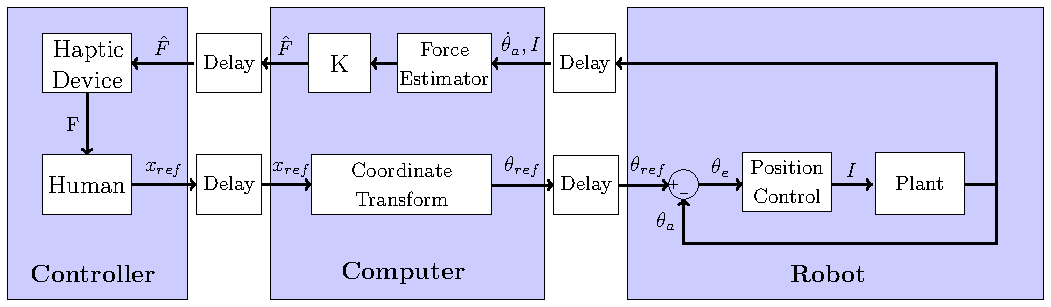
\includegraphics[width=\textwidth]{rapport/pictures/control.pdf} 
	\caption{Simplified block diagram of the control design.}
	\label{fig:simple_control}
\end{figure}

The implemented control loop is made up of two closed loops updating the references of each other. The two main loops are the position control of the robot and the force control of the haptic device. The haptic device's manufacturer did not publish the control architecture of the GT, thus it is treated as a black box which tracks the force references sent to it. The surgeon controlling the GT sets the references for the position loop. The position controller tracks the setpoints and propagate the measured currents to the force estimator. The estimated force is then sent back to the GT as a force reference. 



\begin{figure}[H]
\resizebox{\textwidth}{!}{
	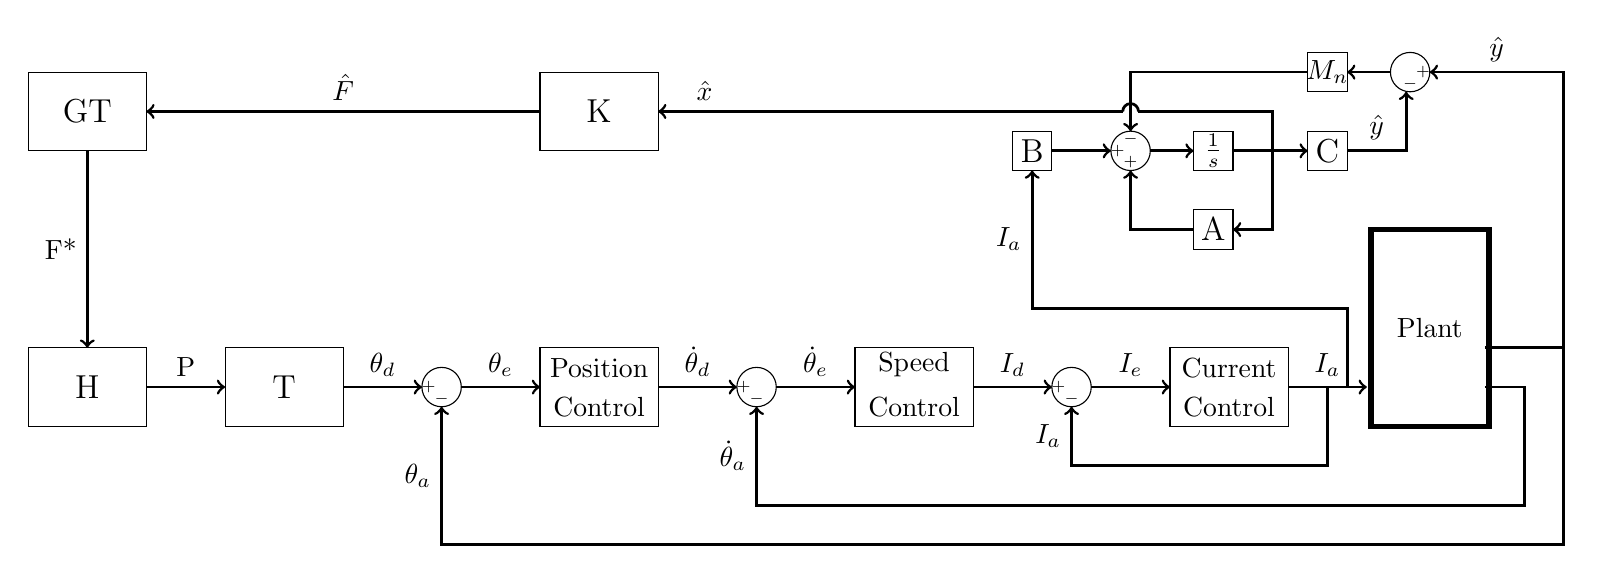
\begin{tikzpicture}
	
	\draw  (0,0) rectangle (1.5,1)node[pos=.5]{\large H};
	\draw  (0,3.5) rectangle (1.5,4.5)node[pos=.5]{\large GT};
	\draw  (6.5,3.5) rectangle (8,4.5)node[pos=.5]{\large K};
	\draw  (2.5,0) rectangle (4,1)node[pos=.5]{\large T};
	\draw  (6.5,0) rectangle (8,1)node[above,pos=.5]{ Position}node[below,pos=.5]{ Control};
	
	
	\draw [->,line width=1pt] (0.75,3.5) -- (0.75,1) node [pos=0.5,left] {F*};
	\draw [->,line width=1pt] (1.5,0.5) -- (2.5,0.5) node [pos=0.5,above] {P};
	\draw [->,line width=1pt] (4,0.5) -- (5,0.5) node [pos=0.5,above] (v1) {$\theta_d$};
	
	\draw [<-,line width=1pt] (1.5,4) -- (6.5,4) node [pos=0.5,above] {$\hat{F}$};
	\draw [<-,line width=1pt] (8,4) -- (13.9,4) node [pos=0.1,above] {$\hat{x}$};
	
	
	;
	
	
	\draw  (5.25,0.5) ellipse (0.25 and 0.25) node  [ left=-0.5mm]{\tiny$+$} node  [below =-0.5mm]{\tiny$-$};
	\draw [->,line width=1pt] (5.5,0.5) -- (6.5,0.5) node [pos=0.5,above] (v1) {$\theta_e$};
	
	
	
	\draw [->,line width=1pt] (8,0.5) -- (9,0.5) node [pos=0.5,above] (v1) {$\dot\theta_d$};
	\draw  (9.25,0.5) ellipse (0.25 and 0.25) node  [ left=-0.5mm]{\tiny$+$} node  [below =-0.5mm]{\tiny$-$};
	\draw  (10.5,0) rectangle (12,1)node[above,pos=.5]{ Speed}node[below,pos=.5]{ Control};
	\draw [->,line width=1pt] (9.5,0.5) -- (10.5,0.5) node [pos=0.5,above] (v1) {$\dot\theta_e$};
	
	\draw [->,line width=1pt] (12,0.5) -- (13,0.5) node [pos=0.5,above] (v1) {$I_d$};
	\draw  (13.25,0.5) ellipse (0.25 and 0.25) node  [ left=-0.5mm]{\tiny$+$} node  [below =-0.5mm]{\tiny$-$};
	\draw  (14.5,0) rectangle (16,1)node[above,pos=.5]{ Current}node[below,pos=.5]{ Control};
	\draw [->,line width=1pt] (13.5,0.5) -- (14.5,0.5) node [pos=0.5,above] (v1) {$I_e$};
	
	\draw [->,line width=1pt] (16,0.5) -- (17,0.5) node [pos=0.5,above] (v1) {$I_a$};
	
	
	\draw  [line width=2pt] (17.05,0) rectangle (18.55,2.5)node[pos=.5]{Plant};
	
	\draw [->,line width=1pt](16.5,0.5) -- (16.5,-0.5) -- (13.25,-0.5) -- node [pos=0.5,left] {$I_a$} (13.25,0.25);
	\draw  [->,line width=1pt](18.5,0.5) -- (19,0.5) -- (19,-1) --(9.25,-1) --  node [pos=0.5,left]{$\dot\theta_a$}  (9.25,0.25);
	\draw [->,line width=1pt] (18.5,1) -- (19.5,1) node (v2) {} -- (19.5,-1.5) -- (5.25,-1.5) --   node [pos=0.5,left]{$\theta_a$}(5.25,0.25);
	
	\draw  (12.5,3.25) rectangle (13,3.75)node[pos=.5]{\large B};
	
	
	
	\draw [<-,line width=1pt](12.75,3.25) -- node [pos=0.5,left]{$I_a$} (12.75,1.5) -- (16.75,1.5) -- (16.75,0.5);
	\draw  (14,3.5) ellipse (0.25 and 0.25) node  [ left=-0.5mm]{\tiny$+$} node  [below =-0.5mm]{\tiny$+$} node  [above =-0.5mm]{\tiny$-$};
	\draw [->,line width=1pt](13,3.5) -- (13.75,3.5);
	
	
	\draw  (14.8,3.25) rectangle (15.3,3.75)node[pos=.5]{$ \frac{1}{s}$};
	\draw [->,line width=1pt](14.25,3.5) -- (14.8,3.5);
	
	\draw  (16.25,3.25) rectangle (16.75,3.75)node[pos=.5]{\large C};
	\draw [->,line width=1pt](15.3,3.5) -- (16.25,3.5);
	
	
	\draw  (14.8,2.25) rectangle (15.3,2.75)node[pos=.5]{\large A};
	
	\draw [->,line width=1pt] (15.8,3.5) -- (15.8,2.5) -- (15.3,2.5);
	
	\draw [->,line width=1pt] (14.8,2.5) -- (14,2.5) -- (14,3.25);\draw  (17.55,4.5) ellipse (0.25 and 0.25) node  [below =-0.5mm]{\tiny$-$} node  [right =-0.5mm]{\tiny$+$};
	
	\draw  (16.25,4.25) rectangle (16.75,4.75)node[pos=.5]{ $M_n$};
	\draw [->,line width=1pt](16.75,3.5) --node[above,pos=.5]{ $\hat y$} (17.5,3.5) -- (17.5,4.25);
	\draw [->,line width=1pt](17.3,4.5) -- (16.75,4.5);
	\draw[->,line width=1pt](16.25,4.5) -- (14,4.5) -- (14,3.75);
	\draw  [->,line width=1pt](19.5,1) -- (19.5,4.5) --node[above,pos=.5]{ $\hat y$} (17.8,4.5);
	\draw [line width=1pt] (15.8,3.5) -- (15.8,4) -- (14.1,4);
	
	
	
	\draw[line width=1pt]  (14.1,4) arc (0:180:0.1);
	\end{tikzpicture}
}
\caption{Overview of the control system}
\label{fig:control_block}
\end{figure}

\section{Human model}
In this section a model of a human arm and hand are derived. This is done because of the \todo{Need something for this}..
%ref
% http://research.vuse.vanderbilt.edu/cim/pubs/journal/13%20-%20Speich%20Shao%20and%20Goldfarb%202005.pdf

The human model can be describe from a mass-spring-damper model\todo{reference}, see figure \todo{figref}. This model has the base position in armpit of the operator. The constants $K_2$, $b_2$ and $K_1$, $b_1$ are the damper and spring constant for the arm and hand respectively. The mass, M, is the arm of the operator and the force, F, is the force between the hand and the manipulator, in this case the Geomagic touch.

\begin{figure}[H]
\centering
\begin{tikzpicture}%[every node/.style={draw,outer sep=0pt,thick}]

\node at (-0.3,0) {$F_h$};
\draw [->,ultra thick] (0,0) -- (1,0);

\draw [ultra thick] (1,-1) rectangle (2,1);
\draw [->,ultra thick] (2,1) -- (2,1.5) -- (2.5,1.5);
\node at (3,1.5) {$x_m$};

\draw [ultra thick] (4,-1) rectangle (5,1);
\draw [->,ultra thick] (5,1) -- (5,1.5) -- (5.5,1.5);
\node at (6,1.5) {$x_h$};


\node at (4.5,0) {$M_h$};

\draw [spring] (2,0.5) -- (4,0.5);
\draw [damper] (2,-0.5) -- (4,-0.5); 
\node at (3,0.9) {$k_1$};
\node at (3,-1.2) {$b_1$};


\draw [spring] (5,0.5) -- (7,0.5);
\draw [damper] (5,-0.5) -- (7,-0.5); 
\node at (6,0.9) {$k_2$};
\node at (6,-1.2) {$b_2$};

\node (wall) [ground, rotate=90, minimum width=3cm] at (7.18,0) {};
\draw (wall.north east) -- (wall.north west);






\end{tikzpicture}
\caption{Simple human arm/hand dynamical model.}
\end{figure}
\todo{add b,K,F and mx and mh direction}




From \todo{figure} the dynamic equations can be derived as \eqref{eq:force_endo_hand2} and \eqref{eq:force_endow_hand}.

\begin{equation}
F_h = k_1(x_m-x_h)+b_1(x_m-x_h)
\label{eq:force_endo_hand2}
\end{equation}

\begin{equation}
m_hx_hs^2 = k_1(x_m-x_h)+b_1(x_m-x_h)s-k_2x_h-b_2x_hs
\label{eq:force_endow_hand}
\end{equation}

By substituting the equations into each other the transfer function for the dynamic model can be found. In this case the transfer function is made for the force between the hand and the Geomagic touch and its position, see \eqref{eq:force_endo_hand3}

\begin{equation}
\frac{x_m}{F_h} = \frac{m_hs^2+(b_2+b_1)s+(k_2+k_1)}{m_hb_1s^3+(m_hk_1+b_1b_2)s^2+(k_1b_2+b_1k_2)s+k_2k_1}
\label{eq:force_endo_hand3}
\end{equation}
\section{Friction model}

In \secref{sec:estimation}, some small forces are fed back to the human leading to oscillations when no external forces are applied. It is suspected that accurately modeling the nonlinearities of the system would improve the transparency of the feedback.  
%The current effort measured by the ESCON controller is \textcolor{green}{proportional} to the sum of the force required to overcome the nonlinearities of the EndoWrist and the external forces applied to the end-effector.
 One of the main nonlinearities is the friction. For the system to be transparent, the force required to overcome friction should not be fed back as this force would not be felt if the teleoperator was holding the tool directly. In order to isolate the external forces, a friction model is required. The model built is based on the one derived in \cite{force_reflection} that describe the friction in a motor. However in the model it was decided to consider the motor and the EndoWrist as one element as no dynamic model for the motor alone is derived. Thus, the model estimates the sum of the friction in the EndoWrist and in the motor.

\subsection{Model}
The total friction acting on the actuator can be written as:
\vspace{9pt}
\begin{equation}
\tau_f = \tau_v + \tau_c + \tau_s
\label{eq:total_friction}
\end{equation} 

with:\\
\hspace*{8mm} $\tau_v$ viscous friction\\
\hspace*{8mm} $\tau_c$ coulomb friction\\
\hspace*{8mm} $\tau_s$ static friction    


The viscous friction is proportional to the opposite of the velocity:
\begin{equation}
\tau_v = F_\mu \cdot \omega
\label{eq:viscous_friction}
\end{equation}
with:\\
\hspace*{8mm}$\omega$ the angular velocity\\
\hspace*{8mm}$F_\mu$ a negative coefficient\\

The coefficient $F_\mu$ can be computed from the measurements made on the setup by plotting the effort depending on the velocity.

The stiction or static friction is the amount of effort required for the object to start moving when its velocity is zero. As such it can be described as:
\vspace{9pt}
\begin{equation} 
\tau_s =  \begin{cases} K_s, & \mbox{if } \omega = 0 \\ 0, & \mbox{else} \end{cases}
\label{eq:static_friction}
\end{equation}
with:\\
\hspace*{8mm}$\omega$ the angular velocity\\
\hspace*{8mm}$K_s$ a constant\\

%The constant $K_s$ can be measured by increasing the current supplied to the motor until it starts moving. 
The coulomb friction occurs as a constant force opposing the movement:

\begin{equation}
\tau_c = sign(\omega)\cdot K_c
\label{eq:coulomb_friction}
\end{equation}
with:\\
\hspace*{8mm}$\omega$ the angular velocity\\
\hspace*{8mm}$K_c$ a constant determined experimentally\\
\hspace*{8mm}the $sign$ function is defined as $sign(\omega) = \begin{cases} 1, & \mbox{if } \omega > 0 \\ 0, & \mbox{if } \omega == 0 \\ -1, & \mbox{if } \omega < 0\end{cases}$\\

%The constant $K_c$ can be measured by setting the motor in motion and decreasing the current until the motor stops moving.
From \eqref{eq:viscous_friction} to \eqref{eq:coulomb_friction}, the total friction given by \eqref{eq:total_friction} can be plotted as:

\begin{figure}[h]
\centering
	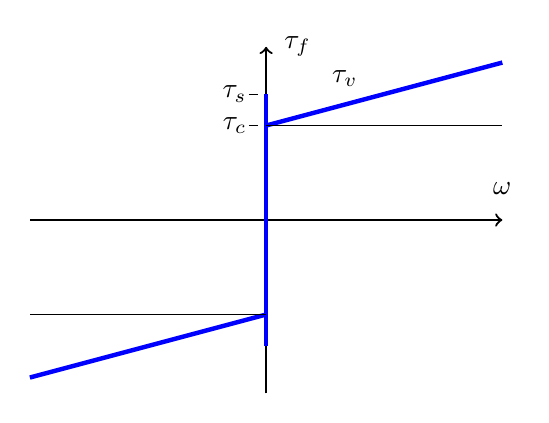
\begin{tikzpicture}
	%axes
	\draw [->,thick] (-3,0) -- (3,0);
	\draw [->,thick] (0,-2.2) -- (0,2.2);
	%friction model
	\draw [ultra thick, color=blue] (0,-1.6) -- (0,1.6);
	\draw [ultra thick, color=blue] (0,1.2) -- (3,2);
	\draw [ultra thick, color=blue] (0,-1.2) -- (-3,-2);
	\draw (0,1.2) -- (3,1.2);
	\draw (0,-1.2) -- (-3,-1.2);
	%name of axis and variables
	\node at (-0.4,1.6) {$\tau_s$};
	\draw (-0.22,1.6) -- (-0.1,1.6);
	\node at (-0.4,1.2) {$\tau_c$};
	\draw (-0.22,1.2) -- (-0.1,1.2);
	\node at (1,1.8) {$\tau_v$};


	\node at (3,0.4) {$\omega$};
	\node at (0.4,2.2) {$\tau_f$};

	\end{tikzpicture}
\caption{friction model}
\end{figure}

\subsection{Measurements}

For the model to be complete, each type of friction requries a value to be measured. These measurements need to be made for each joint as the nonlinearities in the EndoWrist varies greatly depending on the joints.

\subsection*{Test equipment:}

\begin{itemize}
	\item Endowrist model 420093 (AAU number: \#4).
	\item Maxon 110160 motor with attached Maxon gearhead 110356 and Maxon encoder 201937.
	\item sbRIO board.
\end{itemize}

\subsection*{Procedure:}
The viscous friction coefficient $F$ can be calculated by measuring the current for different speeds. From these values, an affine function can be computed, the slope of which will be the coefficient.
The constant $K_c$ for the Coulomb friction can be measured by setting the motor in motion and decreasing the current until it stops moving. The value of the current at that time is the value of $K_c$.
The constant $K_s$ for the static friction is measured by increasing the current sent to the motor until it starts moving. The value of the current at that time is the value of $K_s$.

This procedure is repeated for each motors.

\subsection*{Measuring data:}
\begin{figure}[H]
	\centering
	% This file was created by matlab2tikz.
%
%The latest updates can be retrieved from
%  http://www.mathworks.com/matlabcentral/fileexchange/22022-matlab2tikz-matlab2tikz
%where you can also make suggestions and rate matlab2tikz.
%
\definecolor{mycolor1}{rgb}{0.00000,0.44700,0.74100}%
%
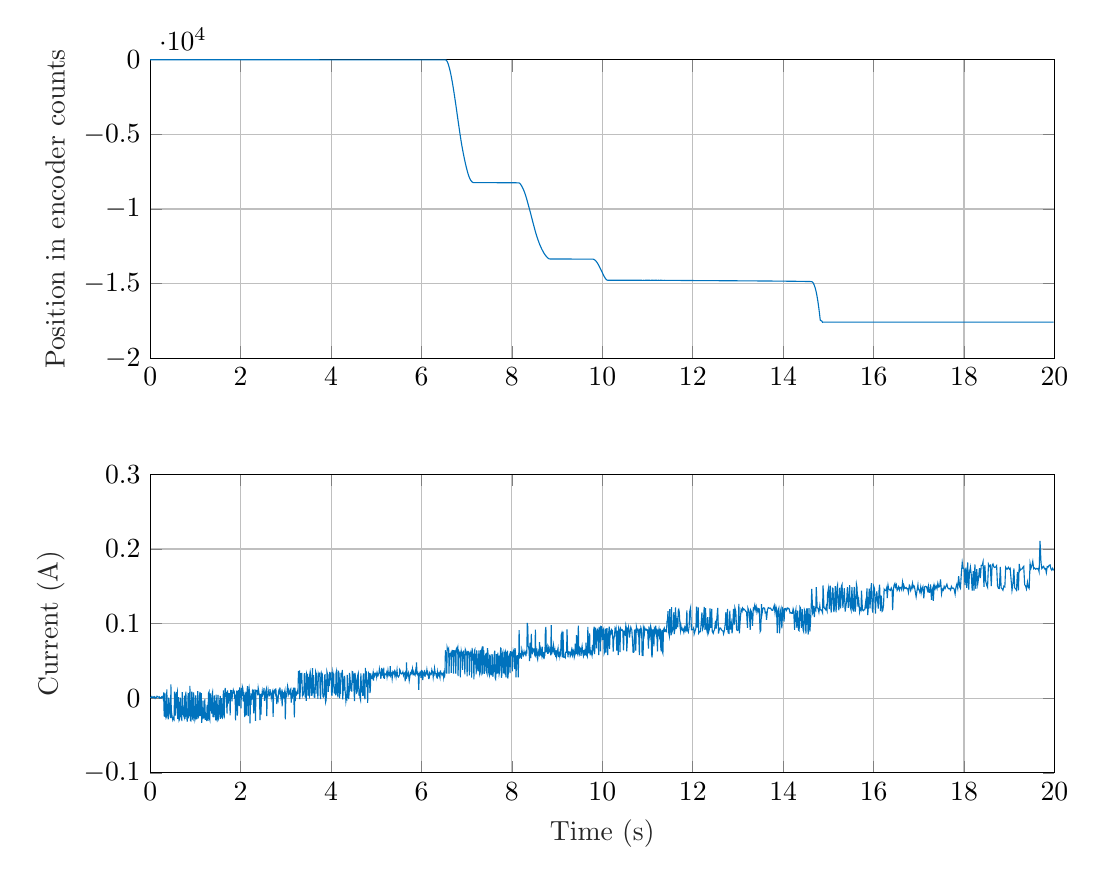
\begin{tikzpicture}

\begin{axis}[%
width=4.521in,
height=1.493in,
at={(0.758in,2.554in)},
scale only axis,
xmin=0,
xmax=20,
ymin=-20000,
ymax=0,
ylabel style={font=\color{white!15!black}},
ylabel={Position in encoder counts},
axis background/.style={fill=white},
xmajorgrids,
ymajorgrids
]
\addplot [color=mycolor1, forget plot]
  table[row sep=crcr]{%
0	0\\
0.02725744	0\\
0.03728676	0\\
0.04958916	0\\
0.05725431	0\\
0.06728411	0\\
0.07726097	0\\
0.08731127	0\\
0.09955502	0\\
0.10726881	0\\
0.11729431	0\\
0.12728214	0\\
0.13732958	0\\
0.14959764	0\\
0.15727186	0\\
0.16730928	0\\
0.17729568	0\\
0.18732214	0\\
0.19960022	0\\
0.20727921	0\\
0.21731997	0\\
0.22730112	0\\
0.23733616	0\\
0.24961329	0\\
0.2572937	0\\
0.26732731	0\\
0.27731371	0\\
0.28735065	0\\
0.29959202	0\\
0.30730677	0\\
0.31734419	0\\
0.32732582	0\\
0.33737564	0\\
0.3496027	0\\
0.35731268	0\\
0.36734486	0\\
0.37733603	0\\
0.38736629	0\\
0.39964342	0\\
0.40732479	0\\
0.41736126	0\\
0.4273448	0\\
0.43737841	0\\
0.44964027	0\\
0.45734119	0\\
0.46736956	0\\
0.4773531	0\\
0.48740482	0\\
0.49970484	0\\
0.50735998	0\\
0.51738071	0\\
0.52736855	0\\
0.5374155	0\\
0.54968071	0\\
0.55737114	0\\
0.56739426	0\\
0.57738066	0\\
0.58742189	0\\
0.59969187	0\\
0.60736847	0\\
0.61739826	0\\
0.62739182	0\\
0.63743448	0\\
0.6498127	0\\
0.6573782	0\\
0.66741371	0\\
0.67740965	0\\
0.68744802	0\\
0.6997385	0\\
0.70739174	0\\
0.71743107	0\\
0.72741556	0\\
0.73748016	0\\
0.74978542	0\\
0.75740576	0\\
0.76743746	0\\
0.77744055	0\\
0.7874999	0\\
0.79983044	0\\
0.80741215	0\\
0.8174634	0\\
0.82744026	0\\
0.83748913	0\\
0.84976864	0\\
0.85742188	0\\
0.86746073	0\\
0.87744856	0\\
0.88750172	0\\
0.89989138	0\\
0.90744638	0\\
0.91746902	0\\
0.92746115	0\\
0.93750048	0\\
0.94980145	0\\
0.9574604	0\\
0.96748018	0\\
0.97746754	0\\
0.98752213	0\\
0.99978924	0\\
1.00746536	0\\
1.01749325	0\\
1.02748632	0\\
1.0375247	0\\
1.04981041	0\\
1.05747461	0\\
1.06752253	0\\
1.07748842	0\\
1.08753395	0\\
1.09983158	0\\
1.10748911	0\\
1.11750937	0\\
1.12750673	0\\
1.137537	0\\
1.14986134	0\\
1.15749264	0\\
1.16752291	0\\
1.17751884	0\\
1.18754292	0\\
1.19987154	0\\
1.20751095	0\\
1.21753025	0\\
1.22752142	0\\
1.23756742	0\\
1.24991846	0\\
1.25751448	0\\
1.26753855	0\\
1.27752399	0\\
1.28757811	0\\
1.29983902	0\\
1.3075285	0\\
1.3175602	0\\
1.32754993	0\\
1.33758974	0\\
1.34985828	0\\
1.35754061	0\\
1.36755753	0\\
1.37754869	0\\
1.38757658	0\\
1.39988708	0\\
1.40755272	0\\
1.41756582	0\\
1.42756033	0\\
1.43759155	0\\
1.44986963	0\\
1.45755911	0\\
1.46758747	0\\
1.47757006	0\\
1.48762417	0\\
1.49995375	0\\
1.50757599	0\\
1.517591	0\\
1.52759027	0\\
1.5376296	0\\
1.54994726	0\\
1.55757904	0\\
1.5676074	0\\
1.57759428	0\\
1.5876379	0\\
1.59994125	0\\
1.60759544	0\\
1.61760998	0\\
1.62760258	0\\
1.63763809	0\\
1.6499691	0\\
1.65760994	0\\
1.6676259	0\\
1.67760849	0\\
1.68766546	0\\
1.69996119	0\\
1.70761538	0\\
1.71763849	0\\
1.72762632	0\\
1.73768377	0\\
1.74998808	0\\
1.75763226	0\\
1.76764488	0\\
1.77765846	0\\
1.78768396	0\\
1.7999773	0\\
1.80764246	0\\
1.81766224	0\\
1.82765484	0\\
1.83767843	0\\
1.84997892	0\\
1.85765696	0\\
1.86767006	-1\\
1.87766504	-1\\
1.88772249	-1\\
1.89998484	-1\\
1.90766525	-1\\
1.91768312	-1\\
1.92766571	-1\\
1.93772316	-1\\
1.95008755	-1\\
1.95768118	-1\\
1.96769381	-1\\
1.97767735	-1\\
1.9877286	-1\\
2.00006914	-1\\
2.00768232	-1\\
2.01770639	-1\\
2.02771091	-1\\
2.0377512	-1\\
2.05007696	-1\\
2.05769682	-1\\
2.06773233	-1\\
2.07771063	-1\\
2.0877862	-1\\
2.10014343	-1\\
2.10772276	-1\\
2.11774588	-1\\
2.12773466	-1\\
2.13776255	-1\\
2.15006304	-1\\
2.15773535	-1\\
2.16773701	-1\\
2.17776012	-1\\
2.18779755	-1\\
2.20014334	-1\\
2.20774651	-1\\
2.21776581	-1\\
2.22776175	-1\\
2.23778963	-1\\
2.25014782	-1\\
2.25775766	-1\\
2.26779127	-1\\
2.27777338	-1\\
2.28781319	-1\\
2.30012703	-1\\
2.30777836	-1\\
2.31779337	-1\\
2.32778883	-1\\
2.33783484	-1\\
2.35015869	-1\\
2.35781622	-1\\
2.36783457	-1\\
2.3778038	-1\\
2.38784266	-1\\
2.40017128	-1\\
2.40781021	-1\\
2.41783667	-1\\
2.42780638	-1\\
2.43785429	-1\\
2.4501996	-1\\
2.45781946	-1\\
2.46783543	-1\\
2.47782564	-1\\
2.48787498	-1\\
2.50026178	-1\\
2.50784159	-1\\
2.5178504	-1\\
2.52784634	-1\\
2.53791094	-1\\
2.55029345	-1\\
2.55784512	-1\\
2.56787443	-1\\
2.57785559	-1\\
2.58791733	-1\\
2.60027218	-1\\
2.60786819	-1\\
2.61789799	-1\\
2.62788057	-1\\
2.63792801	-1\\
2.65031433	-1\\
2.65788841	-1\\
2.66790771	-1\\
2.67788839	-1\\
2.68795252	-1\\
2.70024538	-1\\
2.70792866	-1\\
2.71790791	-1\\
2.7278924	-1\\
2.73795128	-1\\
2.75026894	-1\\
2.75789261	-1\\
2.76792336	-1\\
2.77792072	-1\\
2.78798342	-1\\
2.80033588	-1\\
2.80794954	-1\\
2.81795025	-1\\
2.82794142	-1\\
2.83798265	-1\\
2.8503027	-1\\
2.85794067	-1\\
2.86795473	-1\\
2.87794018	-1\\
2.88801289	-1\\
2.90030289	-1\\
2.90795994	-1\\
2.91795778	-1\\
2.92795038	-1\\
2.93801594	-1\\
2.95028877	-1\\
2.95796776	-1\\
2.96799088	-1\\
2.97798061	-1\\
2.98805714	-1\\
3.00041485	-1\\
3.00797367	-1\\
3.01798964	-1\\
3.02800035	-1\\
3.0381031	-1\\
3.05040216	-1\\
3.0580678	-1\\
3.06806564	-1\\
3.07806015	-1\\
3.08809566	-1\\
3.10037804	-1\\
3.10806704	-1\\
3.11808109	-1\\
3.12807369	-1\\
3.13809919	-1\\
3.15038919	-1\\
3.15806913	-1\\
3.16810703	-1\\
3.17802095	-1\\
3.18810558	-1\\
3.20047665	-1\\
3.20807886	-1\\
3.218081	-1\\
3.22807932	-1\\
3.23812819	-1\\
3.2504859	-1\\
3.25808859	-1\\
3.26809359	-1\\
3.27808952	-1\\
3.28814316	-1\\
3.30047035	-2\\
3.30810452	-2\\
3.31811666	-2\\
3.32810354	-2\\
3.33813477	-2\\
3.35048676	-2\\
3.35811329	-2\\
3.36812353	-2\\
3.37810707	-2\\
3.38816166	-2\\
3.40047741	-2\\
3.40811634	-2\\
3.41812754	-2\\
3.42811108	-2\\
3.43815994	-2\\
3.45046282	-3\\
3.45814037	-3\\
3.46814585	-3\\
3.47812176	-3\\
3.48816395	-3\\
3.50047016	-3\\
3.50814581	-3\\
3.51816034	-3\\
3.52815056	-3\\
3.53818417	-3\\
3.55045748	-3\\
3.5581522	-3\\
3.5681653	-3\\
3.57816029	-3\\
3.58819866	-3\\
3.60050106	-4\\
3.60816956	-4\\
3.61817741	-4\\
3.62817383	-4\\
3.63821268	-4\\
3.65048647	-4\\
3.65816307	-4\\
3.66818476	-4\\
3.67818165	-4\\
3.68822861	-5\\
3.7005806	-5\\
3.70818615	-5\\
3.71819878	-6\\
3.72817564	-6\\
3.73823261	-6\\
3.7505331	-7\\
3.75820637	-7\\
3.76821423	-7\\
3.7782445	-7\\
3.78825235	-7\\
3.80058861	-7\\
3.80822086	-7\\
3.81823111	-7\\
3.82821798	-7\\
3.83823109	-7\\
3.85059881	-7\\
3.85821819	-7\\
3.8682394	-7\\
3.87820721	-7\\
3.88825083	-7\\
3.90063906	-7\\
3.90823269	-7\\
3.91824293	-7\\
3.92825508	-7\\
3.93828154	-7\\
3.95054531	-7\\
3.95822716	-7\\
3.96826553	-7\\
3.97822762	-7\\
3.98829365	-7\\
4.00064039	-7\\
4.00823689	-7\\
4.01827002	-7\\
4.02827644	-7\\
4.03828812	-7\\
4.05064392	-7\\
4.05827236	-7\\
4.06826973	-7\\
4.07827187	-7\\
4.08830833	-7\\
4.10061121	-7\\
4.10830784	-7\\
4.11827087	-7\\
4.12826443	-7\\
4.13842106	-7\\
4.15068388	-7\\
4.15828276	-7\\
4.1682868	-7\\
4.1782918	-7\\
4.18835211	-7\\
4.20065784	-7\\
4.2083087	-7\\
4.21830177	-7\\
4.22833776	-7\\
4.23835897	-7\\
4.25068474	-7\\
4.25831842	-7\\
4.26834917	-7\\
4.27830124	-7\\
4.28846264	-7\\
4.30070925	-7\\
4.30832148	-7\\
4.31832457	-7\\
4.32832575	-7\\
4.33838415	-7\\
4.35064697	-7\\
4.35832787	-7\\
4.36833286	-7\\
4.37834597	-7\\
4.38840628	-7\\
4.40074444	-7\\
4.4083848	-7\\
4.41836882	-7\\
4.42836189	-7\\
4.43838263	-7\\
4.45071602	-7\\
4.45836735	-7\\
4.46838427	-7\\
4.47837162	-7\\
4.48842621	-7\\
4.50073242	-7\\
4.50838947	-7\\
4.51838446	-7\\
4.52837896	-7\\
4.53845787	-7\\
4.55077457	-7\\
4.55840349	-7\\
4.56841898	-7\\
4.57838774	-7\\
4.58843136	-7\\
4.6007638	-7\\
4.60841608	-7\\
4.61841488	-7\\
4.62841892	-7\\
4.63843966	-7\\
4.650702	-7\\
4.65842342	-7\\
4.66844797	-7\\
4.67841291	-7\\
4.68843174	-7\\
4.70075607	-7\\
4.70840502	-7\\
4.71843863	-7\\
4.72842598	-7\\
4.73847914	-7\\
4.75078917	-7\\
4.75844812	-7\\
4.76846743	-7\\
4.77845478	-7\\
4.788517	-7\\
4.80076933	-7\\
4.80845261	-7\\
4.8184762	-7\\
4.82859468	-7\\
4.83850861	-7\\
4.85076666	-7\\
4.85847712	-7\\
4.86850119	-7\\
4.87848282	-7\\
4.88854122	-7\\
4.90080404	-7\\
4.90849972	-7\\
4.91850853	-7\\
4.92850018	-7\\
4.93854952	-7\\
4.95085001	-7\\
4.95849705	-7\\
4.96851254	-7\\
4.97850561	-7\\
4.98855495	-7\\
5.00091934	-7\\
5.00847435	-7\\
5.0185194	-7\\
5.0285306	-7\\
5.03855419	-7\\
5.05085039	-7\\
5.05851555	-7\\
5.06855011	-7\\
5.07851601	-7\\
5.08857393	-7\\
5.10083485	-7\\
5.10853815	-7\\
5.11854172	-7\\
5.12864304	-7\\
5.13858128	-7\\
5.15094662	-7\\
5.15852404	-7\\
5.16854095	-7\\
5.17853689	-7\\
5.18855715	-7\\
5.20088625	-7\\
5.20857716	-7\\
5.2185626	-7\\
5.22854853	-7\\
5.23856783	-7\\
5.25096083	-7\\
5.25852966	-7\\
5.26858139	-7\\
5.27854872	-7\\
5.28857803	-7\\
5.30090952	-8\\
5.30858421	-8\\
5.31856108	-8\\
5.32855415	-8\\
5.33861113	-8\\
5.35091829	-8\\
5.35857916	-8\\
5.36864567	-8\\
5.37857485	-8\\
5.38865423	-8\\
5.4009037	-8\\
5.40857172	-8\\
5.4186182	-8\\
5.42860794	-8\\
5.43861628	-8\\
5.45098829	-8\\
5.45860386	-8\\
5.46863651	-8\\
5.47857904	-8\\
5.48864317	-8\\
5.50100851	-8\\
5.5086174	-8\\
5.51864529	-8\\
5.52861357	-8\\
5.53864717	-8\\
5.55098486	-8\\
5.55859852	-8\\
5.56862593	-8\\
5.5786109	-8\\
5.58865404	-8\\
5.60104561	-8\\
5.60864019	-8\\
5.61865807	-8\\
5.62866545	-8\\
5.63865852	-8\\
5.65093803	-8\\
5.65862226	-8\\
5.66866493	-8\\
5.67864895	-8\\
5.68864727	-8\\
5.70098066	-8\\
5.70867586	-8\\
5.71866417	-8\\
5.72865582	-8\\
5.7386961	-8\\
5.75109148	-8\\
5.75867319	-8\\
5.76868868	-8\\
5.77867699	-8\\
5.78874588	-8\\
5.80100203	-8\\
5.80865431	-8\\
5.81868172	-8\\
5.82868528	-8\\
5.83871508	-8\\
5.85110283	-8\\
5.85869789	-8\\
5.86873102	-8\\
5.8787055	-8\\
5.88871431	-8\\
5.9010191	-8\\
5.90872145	-8\\
5.91873121	-8\\
5.9287014	-8\\
5.93876743	-8\\
5.95114517	-8\\
5.95870733	-8\\
5.96872759	-8\\
5.97870111	-8\\
5.98875332	-8\\
6.00107765	-8\\
6.00873756	-8\\
6.0187397	-8\\
6.02878761	-8\\
6.03878927	-8\\
6.05113316	-8\\
6.05872965	-8\\
6.06877041	-8\\
6.07874203	-8\\
6.0888195	-8\\
6.10108519	-8\\
6.10879755	-8\\
6.11877155	-8\\
6.12875366	-8\\
6.1388154	-8\\
6.15115833	-8\\
6.15873194	-8\\
6.16877031	-8\\
6.17876577	-8\\
6.18883324	-8\\
6.20111275	-8\\
6.20875978	-8\\
6.21877193	-8\\
6.22875261	-8\\
6.2388339	-8\\
6.25116682	-8\\
6.25876999	-8\\
6.26883411	-8\\
6.27878046	-8\\
6.28884172	-8\\
6.30119801	-8\\
6.30882406	-8\\
6.31881809	-8\\
6.32879496	-8\\
6.33888912	-8\\
6.35120964	-8\\
6.35877037	-8\\
6.36883402	-8\\
6.3788147	-8\\
6.38888121	-8\\
6.40122318	-8\\
6.40881157	-8\\
6.41882658	-8\\
6.4288435	-8\\
6.43883324	-8\\
6.45116901	-8\\
6.45879555	-8\\
6.46886063	-8\\
6.47883463	-8\\
6.48889637	-8\\
6.50127983	-8\\
6.50883293	-8\\
6.5188899	-8\\
6.52886915	-8\\
6.53884554	-17\\
6.55124474	-45\\
6.55882311	-76\\
6.56886864	-128\\
6.57884645	-195\\
6.58892632	-275\\
6.60120058	-389\\
6.60883808	-469\\
6.61892176	-583\\
6.62886477	-704\\
6.63891697	-838\\
6.6512351	-1012\\
6.65886641	-1129\\
6.66894102	-1290\\
6.67886066	-1459\\
6.68890142	-1639\\
6.70140696	-1867\\
6.70889902	-2007\\
6.71892309	-2200\\
6.72890568	-2396\\
6.73893976	-2600\\
6.75148058	-2857\\
6.75886679	-3009\\
6.76893473	-3226\\
6.77896166	-3440\\
6.7889986	-3657\\
6.80126143	-3917\\
6.80890083	-4079\\
6.81896257	-4290\\
6.82895803	-4501\\
6.8389554	-4711\\
6.85142803	-4966\\
6.85890675	-5117\\
6.86894846	-5314\\
6.87894106	-5505\\
6.888978	-5687\\
6.90128469	-5896\\
6.90893936	-6024\\
6.91895247	-6185\\
6.92894077	-6339\\
6.93898916	-6490\\
6.95135069	-6670\\
6.95893955	-6779\\
6.96898746	-6918\\
6.97895193	-7047\\
6.98901749	-7177\\
7.00132513	-7327\\
7.00899172	-7414\\
7.01900053	-7524\\
7.02905464	-7628\\
7.03901052	-7725\\
7.05134583	-7831\\
7.05896425	-7891\\
7.06905985	-7963\\
7.07900667	-8024\\
7.08904409	-8077\\
7.10140133	-8126\\
7.10899878	-8152\\
7.11905861	-8183\\
7.12906408	-8207\\
7.13907433	-8222\\
7.15145636	-8231\\
7.15900993	-8233\\
7.16905785	-8233\\
7.17900419	-8233\\
7.18910265	-8233\\
7.20141363	-8233\\
7.20901346	-8233\\
7.21907949	-8233\\
7.22910213	-8234\\
7.23911428	-8234\\
7.25142479	-8234\\
7.25904465	-8234\\
7.26912928	-8234\\
7.27908516	-8234\\
7.2891202	-8234\\
7.30145454	-8234\\
7.30907917	-8234\\
7.31907892	-8235\\
7.32905054	-8235\\
7.33913326	-8235\\
7.35147524	-8235\\
7.35904551	-8235\\
7.36913538	-8235\\
7.37907171	-8235\\
7.38915014	-8235\\
7.40148973	-8235\\
7.40907574	-8235\\
7.41913366	-8235\\
7.42908621	-8235\\
7.43914127	-8235\\
7.45142078	-8235\\
7.45908022	-8236\\
7.46912289	-8236\\
7.47908258	-8236\\
7.48910284	-8236\\
7.50155354	-8236\\
7.50909662	-8236\\
7.51914454	-8236\\
7.52911854	-8236\\
7.53933144	-8236\\
7.55150414	-8236\\
7.55911684	-8236\\
7.56913805	-8236\\
7.57913113	-8236\\
7.58917475	-8236\\
7.60152149	-8237\\
7.60909224	-8237\\
7.61913681	-8237\\
7.62912416	-8237\\
7.63915205	-8237\\
7.65151834	-8237\\
7.65910339	-8237\\
7.66914797	-8238\\
7.67912388	-8238\\
7.68920183	-8238\\
7.70150471	-8238\\
7.70919371	-8239\\
7.71917868	-8239\\
7.7291646	-8239\\
7.73918295	-8240\\
7.75152636	-8240\\
7.75914145	-8240\\
7.76919317	-8240\\
7.77918243	-8240\\
7.78921175	-8240\\
7.80147171	-8240\\
7.80919075	-8240\\
7.81922007	-8240\\
7.82921314	-8240\\
7.83943558	-8240\\
7.85157776	-8240\\
7.85917234	-8240\\
7.8692503	-8240\\
7.87918472	-8240\\
7.88925552	-8240\\
7.90149164	-8241\\
7.90921545	-8241\\
7.91920662	-8241\\
7.92924166	-8240\\
7.93919945	-8240\\
7.9516449	-8241\\
7.95916891	-8241\\
7.96922731	-8241\\
7.97920227	-8241\\
7.98922634	-8241\\
8.00157166	-8241\\
8.00924301	-8241\\
8.01926517	-8242\\
8.02929497	-8242\\
8.03924751	-8242\\
8.051651	-8243\\
8.05919266	-8243\\
8.06928158	-8243\\
8.07923317	-8244\\
8.08929062	-8244\\
8.10168362	-8245\\
8.10927391	-8245\\
8.11928558	-8245\\
8.12926674	-8245\\
8.1392622	-8246\\
8.15158558	-8247\\
8.15924072	-8253\\
8.16934013	-8273\\
8.17925262	-8300\\
8.18934631	-8337\\
8.20159626	-8388\\
8.2092371	-8424\\
8.21928978	-8476\\
8.2293129	-8534\\
8.23929024	-8594\\
8.25165558	-8674\\
8.2592659	-8729\\
8.26934052	-8805\\
8.27931786	-8886\\
8.28935051	-8972\\
8.30162239	-9080\\
8.30928802	-9153\\
8.3192997	-9254\\
8.32935905	-9360\\
8.33931732	-9465\\
8.35162926	-9603\\
8.35933495	-9688\\
8.36934566	-9800\\
8.37937546	-9908\\
8.38935089	-10019\\
8.4016552	-10155\\
8.40937042	-10241\\
8.41936779	-10359\\
8.42940903	-10478\\
8.43932915	-10596\\
8.45170593	-10745\\
8.45931911	-10836\\
8.46935558	-10951\\
8.47931957	-11065\\
8.48940659	-11179\\
8.50180817	-11319\\
8.50933838	-11403\\
8.51932526	-11509\\
8.52934647	-11616\\
8.53937721	-11719\\
8.55179119	-11842\\
8.5593214	-11909\\
8.56941414	-11999\\
8.57938766	-12085\\
8.58946609	-12171\\
8.60175323	-12271\\
8.60938454	-12332\\
8.61938286	-12408\\
8.62936592	-12479\\
8.63941956	-12549\\
8.65174961	-12630\\
8.65936089	-12677\\
8.66946602	-12737\\
8.67936707	-12794\\
8.68947983	-12852\\
8.70170593	-12919\\
8.70933723	-12959\\
8.71942806	-13007\\
8.72949505	-13051\\
8.73944664	-13092\\
8.75177383	-13139\\
8.75937843	-13167\\
8.76944351	-13203\\
8.77935982	-13233\\
8.7894516	-13261\\
8.80187607	-13296\\
8.80945587	-13314\\
8.81946754	-13332\\
8.82973957	-13341\\
8.83942032	-13345\\
8.85184097	-13345\\
8.85942841	-13345\\
8.86948299	-13345\\
8.87944412	-13345\\
8.88943386	-13345\\
8.9017334	-13346\\
8.91947556	-13346\\
8.92937088	-13346\\
8.93949604	-13346\\
8.95173836	-13346\\
8.96943092	-13346\\
8.97940731	-13347\\
8.98948002	-13347\\
9.00183582	-13347\\
9.0194931	-13347\\
9.02965164	-13347\\
9.03947926	-13347\\
9.05174637	-13347\\
9.05944824	-13347\\
9.06949425	-13348\\
9.07952499	-13348\\
9.08951569	-13348\\
9.10188866	-13348\\
9.11947155	-13348\\
9.12947464	-13348\\
9.13947201	-13349\\
9.15185165	-13349\\
9.16948509	-13349\\
9.17951965	-13349\\
9.18950748	-13350\\
9.2019043	-13350\\
9.20948315	-13350\\
9.21955109	-13350\\
9.22949028	-13350\\
9.23953819	-13350\\
9.25191307	-13351\\
9.2694931	-13351\\
9.27949047	-13351\\
9.28955841	-13351\\
9.30187607	-13351\\
9.31953049	-13352\\
9.32949066	-13352\\
9.33952332	-13352\\
9.35189629	-13352\\
9.36951256	-13352\\
9.37951469	-13353\\
9.38961411	-13353\\
9.40190029	-13353\\
9.40957451	-13353\\
9.41958237	-13353\\
9.42955971	-13353\\
9.43956661	-13353\\
9.45198536	-13353\\
9.46955872	-13353\\
9.47959709	-13354\\
9.48961163	-13354\\
9.50199509	-13354\\
9.51954842	-13354\\
9.52959824	-13354\\
9.53962708	-13354\\
9.55195808	-13354\\
9.56957531	-13355\\
9.58030128	-13355\\
9.58959007	-13355\\
9.602005	-13355\\
9.60962296	-13355\\
9.619627	-13355\\
9.62965202	-13355\\
9.63962364	-13355\\
9.65196609	-13355\\
9.66963005	-13355\\
9.67961693	-13355\\
9.68967247	-13355\\
9.70196342	-13355\\
9.71961594	-13355\\
9.72963428	-13355\\
9.73967552	-13355\\
9.75206947	-13356\\
9.76965332	-13356\\
9.7803154	-13356\\
9.78966713	-13358\\
9.80198574	-13364\\
9.80966854	-13371\\
9.81966972	-13386\\
9.82972717	-13407\\
9.83971596	-13432\\
9.85209751	-13467\\
9.86964607	-13530\\
9.87968731	-13569\\
9.88968468	-13613\\
9.90208626	-13675\\
9.91964531	-13770\\
9.9296999	-13826\\
9.93971252	-13887\\
9.95207977	-13960\\
9.95965958	-14006\\
9.96968842	-14068\\
9.97966671	-14132\\
9.98967934	-14198\\
10.00198936	-14275\\
10.01967049	-14390\\
10.02967358	-14452\\
10.03971291	-14510\\
10.05204868	-14576\\
10.06970215	-14658\\
10.07966328	-14698\\
10.08968163	-14730\\
10.1020174	-14758\\
10.11966896	-14774\\
10.12967205	-14774\\
10.13974094	-14774\\
10.15206337	-14774\\
10.15973854	-14774\\
10.16967869	-14774\\
10.17969894	-14774\\
10.18970871	-14774\\
10.2021246	-14774\\
10.21968937	-14774\\
10.229743	-14774\\
10.23972321	-14774\\
10.25213814	-14774\\
10.26968384	-14774\\
10.27973557	-14774\\
10.28972721	-14774\\
10.30209637	-14774\\
10.31970215	-14775\\
10.33080959	-14775\\
10.33969402	-14775\\
10.35216331	-14775\\
10.35969925	-14775\\
10.36973095	-14775\\
10.37974548	-14775\\
10.38973427	-14775\\
10.40205288	-14775\\
10.41976547	-14775\\
10.42970181	-14775\\
10.43977451	-14775\\
10.45200729	-14775\\
10.46971893	-14775\\
10.47972298	-14775\\
10.48999977	-14775\\
10.50210762	-14775\\
10.51979065	-14775\\
10.53091145	-14775\\
10.53984451	-14775\\
10.55210114	-14775\\
10.5597229	-14775\\
10.56978035	-14775\\
10.579813	-14775\\
10.58978462	-14775\\
10.60218143	-14775\\
10.61975098	-14775\\
10.62979126	-14775\\
10.63976288	-14775\\
10.65215874	-14775\\
10.66976166	-14775\\
10.67982864	-14775\\
10.6897583	-14775\\
10.70218754	-14775\\
10.70979023	-14775\\
10.71989441	-14775\\
10.72976494	-14775\\
10.73980713	-14775\\
10.75222111	-14775\\
10.76978016	-14775\\
10.77978611	-14775\\
10.78984928	-14775\\
10.80212975	-14775\\
10.81981564	-14775\\
10.8297863	-14775\\
10.83978462	-14775\\
10.85213089	-14775\\
10.86979675	-14775\\
10.87981987	-14776\\
10.88986206	-14776\\
10.90208912	-14776\\
10.90981293	-14775\\
10.91982937	-14775\\
10.92982674	-14776\\
10.93985558	-14776\\
10.9522047	-14775\\
10.96982956	-14775\\
10.97996712	-14775\\
10.98982716	-14775\\
11.00222492	-14775\\
11.01981258	-14775\\
11.02990341	-14775\\
11.03984833	-14775\\
11.05230522	-14775\\
11.0698576	-14776\\
11.08141327	-14775\\
11.08984852	-14775\\
11.10217381	-14775\\
11.10983658	-14775\\
11.1198597	-14775\\
11.13012314	-14775\\
11.13994312	-14776\\
11.15214539	-14775\\
11.16997147	-14775\\
11.1800909	-14775\\
11.18991661	-14775\\
11.20220661	-14775\\
11.21988297	-14776\\
11.22987175	-14775\\
11.23994064	-14775\\
11.2522707	-14775\\
11.26999283	-14776\\
11.28159714	-14775\\
11.28990459	-14775\\
11.30212784	-14776\\
11.30984497	-14775\\
11.3199482	-14775\\
11.33048153	-14776\\
11.33993244	-14776\\
11.35231209	-14776\\
11.36989403	-14775\\
11.3804493	-14776\\
11.38994026	-14776\\
11.40234375	-14776\\
11.41993904	-14776\\
11.43045425	-14776\\
11.43994045	-14776\\
11.45238686	-14777\\
11.46993065	-14777\\
11.48158646	-14778\\
11.48991585	-14778\\
11.50234413	-14778\\
11.51993179	-14779\\
11.53165436	-14779\\
11.53994942	-14779\\
11.55230618	-14779\\
11.56990814	-14780\\
11.58176231	-14780\\
11.58992386	-14781\\
11.60225105	-14781\\
11.61993885	-14781\\
11.63168907	-14782\\
11.63996124	-14782\\
11.65229225	-14782\\
11.66996574	-14783\\
11.68059921	-14783\\
11.68996334	-14783\\
11.70240974	-14784\\
11.71994114	-14784\\
11.73041534	-14785\\
11.73998451	-14785\\
11.75249863	-14785\\
11.77000713	-14786\\
11.78069305	-14786\\
11.80232811	-14786\\
11.82006931	-14787\\
11.83180046	-14787\\
11.84000969	-14787\\
11.852314	-14787\\
11.87006569	-14788\\
11.88054466	-14788\\
11.89001656	-14789\\
11.90239239	-14789\\
11.92004967	-14790\\
11.93061256	-14790\\
11.95240402	-14791\\
11.9700489	-14791\\
11.98205376	-14792\\
12.00244904	-14792\\
12.02007484	-14792\\
12.03070831	-14793\\
12.05240536	-14793\\
12.07006836	-14793\\
12.08215618	-14793\\
12.10243034	-14794\\
12.12011528	-14794\\
12.1320858	-14794\\
12.15240765	-14794\\
12.17002106	-14795\\
12.18075466	-14795\\
12.202384	-14795\\
12.22013283	-14796\\
12.23208141	-14796\\
12.25255013	-14796\\
12.27006435	-14796\\
12.28082275	-14796\\
12.30246639	-14797\\
12.32012939	-14797\\
12.33216286	-14797\\
12.35247993	-14798\\
12.37008476	-14798\\
12.38238907	-14798\\
12.40239429	-14798\\
12.42014313	-14799\\
12.43075943	-14799\\
12.45251083	-14799\\
12.47013474	-14799\\
12.48242283	-14800\\
12.50250626	-14800\\
12.52017784	-14800\\
12.53092194	-14801\\
12.55247498	-14801\\
12.57011604	-14801\\
12.58243465	-14802\\
12.60244179	-14802\\
12.62018681	-14802\\
12.63084984	-14803\\
12.6525135	-14803\\
12.6701498	-14803\\
12.68091965	-14803\\
12.70252228	-14804\\
12.72019291	-14804\\
12.7324276	-14804\\
12.75262451	-14804\\
12.77016735	-14805\\
12.78107643	-14805\\
12.8025589	-14805\\
12.82021332	-14806\\
12.8324585	-14806\\
12.85256767	-14806\\
12.87016869	-14807\\
12.88114929	-14807\\
12.90257454	-14807\\
12.92026711	-14807\\
12.93108749	-14808\\
12.95248985	-14808\\
12.97018528	-14808\\
12.99024296	-14809\\
13.00264549	-14809\\
13.02025795	-14810\\
13.03115273	-14810\\
13.05257034	-14811\\
13.07019424	-14811\\
13.09023666	-14812\\
13.10256577	-14812\\
13.12026501	-14813\\
13.1310997	-14813\\
13.15257263	-14813\\
13.17019844	-14813\\
13.19026184	-14814\\
13.21019554	-14814\\
13.22022057	-14814\\
13.24022102	-14815\\
13.25272083	-14815\\
13.27022076	-14815\\
13.28131866	-14815\\
13.30255222	-14816\\
13.3202734	-14816\\
13.3402195	-14817\\
13.3526535	-14817\\
13.37022972	-14817\\
13.3814888	-14817\\
13.40262794	-14818\\
13.42036819	-14818\\
13.44022942	-14819\\
13.46059799	-14819\\
13.47022438	-14819\\
13.49027538	-14819\\
13.50276089	-14820\\
13.52031422	-14820\\
13.53130627	-14820\\
13.55270195	-14821\\
13.57024956	-14821\\
13.59032059	-14821\\
13.60259819	-14822\\
13.62030315	-14822\\
13.63134193	-14822\\
13.65263748	-14823\\
13.67030144	-14823\\
13.69032192	-14824\\
13.7026825	-14824\\
13.72034073	-14824\\
13.74027443	-14825\\
13.75272942	-14825\\
13.77032375	-14826\\
13.78141785	-14826\\
13.8026495	-14826\\
13.82040787	-14827\\
13.84029579	-14827\\
13.85280132	-14828\\
13.87026215	-14828\\
13.88157082	-14829\\
13.90258312	-14829\\
13.92033863	-14830\\
13.94030571	-14831\\
13.95260239	-14831\\
13.97060299	-14832\\
13.99038124	-14832\\
14.0027256	-14833\\
14.02035713	-14834\\
14.03149796	-14834\\
14.05265141	-14834\\
14.07030487	-14835\\
14.09037399	-14836\\
14.10269833	-14836\\
14.12040329	-14837\\
14.13157845	-14837\\
14.15266514	-14838\\
14.17034721	-14839\\
14.1903553	-14839\\
14.20273781	-14839\\
14.22041512	-14840\\
14.23165321	-14840\\
14.25279713	-14841\\
14.27032471	-14842\\
14.28170967	-14842\\
14.30268383	-14843\\
14.3203392	-14844\\
14.3403616	-14845\\
14.35264015	-14846\\
14.37037563	-14846\\
14.38191223	-14847\\
14.40272331	-14848\\
14.42040443	-14848\\
14.44034958	-14849\\
14.45269203	-14850\\
14.47069359	-14851\\
14.48219872	-14852\\
14.5028019	-14853\\
14.5204649	-14853\\
14.53179741	-14854\\
14.55278969	-14855\\
14.57038403	-14856\\
14.59043312	-14858\\
14.60260391	-14859\\
14.62047577	-14862\\
14.63193893	-14865\\
14.65284824	-14906\\
14.67041492	-14984\\
14.69046783	-15124\\
14.70259094	-15231\\
14.72045517	-15429\\
14.73200798	-15578\\
14.75288963	-15905\\
14.77043056	-16241\\
14.7905426	-16684\\
14.81044579	-17179\\
14.82050514	-17448\\
14.84046364	-17484\\
14.85271072	-17498\\
14.87045479	-17585\\
14.88216114	-17580\\
14.90283966	-17580\\
14.92050934	-17580\\
14.94042778	-17580\\
14.95266533	-17580\\
14.9704237	-17580\\
14.98213387	-17580\\
15.00290298	-17580\\
15.02053452	-17580\\
15.04049873	-17580\\
15.06054306	-17580\\
15.07043266	-17580\\
15.09076309	-17580\\
15.10272026	-17580\\
15.12051678	-17580\\
15.13218784	-17580\\
15.15292168	-17580\\
15.17050648	-17580\\
15.19054794	-17580\\
15.20266724	-17580\\
15.22052383	-17580\\
15.23214817	-17580\\
15.25287437	-17580\\
15.27051735	-17580\\
15.29055786	-17580\\
15.30270195	-17580\\
15.32056999	-17580\\
15.34047699	-17580\\
15.35271454	-17580\\
15.3704834	-17580\\
15.38215637	-17580\\
15.40280628	-17580\\
15.42058945	-17580\\
15.44053078	-17580\\
15.45279884	-17580\\
15.47047997	-17580\\
15.48227882	-17580\\
15.50283146	-17580\\
15.52057076	-17580\\
15.54054642	-17580\\
15.55282402	-17580\\
15.57053566	-17580\\
15.59060764	-17580\\
15.6027298	-17580\\
15.62058735	-17580\\
15.63236237	-17580\\
15.65286922	-17580\\
15.67058086	-17580\\
15.6906147	-17580\\
15.70279121	-17580\\
15.72062492	-17580\\
15.73236465	-17580\\
15.75296497	-17580\\
15.77054596	-17580\\
15.79060555	-17580\\
15.80277157	-17580\\
15.82063675	-17580\\
15.83241081	-17580\\
15.85295677	-17580\\
15.87058735	-17580\\
15.88243866	-17580\\
15.90289879	-17580\\
15.92062187	-17580\\
15.94059753	-17580\\
15.95286751	-17580\\
15.97061348	-17580\\
15.98269463	-17580\\
16.00289345	-17580\\
16.02065659	-17580\\
16.04058838	-17580\\
16.0528965	-17580\\
16.07062721	-17580\\
16.08269882	-17580\\
16.10294533	-17580\\
16.1206913	-17580\\
16.13262558	-17580\\
16.15290451	-17580\\
16.1706028	-17580\\
16.19067574	-17580\\
16.20290375	-17580\\
16.22070885	-17580\\
16.23267746	-17580\\
16.25305748	-17580\\
16.2706337	-17580\\
16.29069519	-17580\\
16.30283546	-17580\\
16.32070923	-17580\\
16.33276176	-17580\\
16.35308456	-17580\\
16.37072945	-17580\\
16.39074135	-17580\\
16.41063309	-17580\\
16.42072487	-17580\\
16.44060898	-17580\\
16.45281982	-17580\\
16.47062111	-17580\\
16.48269653	-17580\\
16.50306511	-17580\\
16.52076912	-17580\\
16.54068375	-17580\\
16.55291748	-17580\\
16.57069778	-17580\\
16.58298683	-17580\\
16.60296249	-17580\\
16.62078667	-17580\\
16.64070892	-17580\\
16.66078186	-17580\\
16.67070007	-17580\\
16.69071579	-17580\\
16.70287323	-17580\\
16.72064972	-17580\\
16.73277473	-17580\\
16.753088	-17580\\
16.77075958	-17580\\
16.79081154	-17580\\
16.80287552	-17580\\
16.82071686	-17580\\
16.84076881	-17580\\
16.86075783	-17580\\
16.87079239	-17580\\
16.8907547	-17580\\
16.90300369	-17580\\
16.92084122	-17580\\
16.9407692	-17580\\
16.96084595	-17580\\
16.98069954	-17580\\
16.99071503	-17580\\
17.01070404	-17580\\
17.02075386	-17580\\
17.04080391	-17580\\
17.05311012	-17580\\
17.07080269	-17580\\
17.09078979	-17580\\
17.11074829	-17580\\
17.13085175	-17580\\
17.15310478	-17580\\
17.17087555	-17580\\
17.1908226	-17580\\
17.21087074	-17580\\
17.22075844	-17580\\
17.24082756	-17580\\
17.26080322	-17580\\
17.28071976	-17580\\
17.29078484	-17580\\
17.31083298	-17580\\
17.3208046	-17580\\
17.34087753	-17580\\
17.36078072	-17580\\
17.38074875	-17580\\
17.403162	-17580\\
17.42083168	-17580\\
17.44081116	-17580\\
17.4608593	-17580\\
17.48082352	-17580\\
17.50321198	-17580\\
17.52085876	-17580\\
17.5408783	-17580\\
17.56088638	-17580\\
17.58087921	-17580\\
17.60313797	-17580\\
17.6208725	-17580\\
17.64089012	-17580\\
17.66090775	-17580\\
17.68081284	-17580\\
17.70319939	-17580\\
17.72081184	-17580\\
17.74088097	-17580\\
17.76078796	-17580\\
17.7808876	-17580\\
17.80330276	-17580\\
17.82092667	-17580\\
17.84089279	-17580\\
17.86094856	-17580\\
17.88088226	-17580\\
17.90318108	-17580\\
17.92089844	-17580\\
17.9409008	-17580\\
17.96086884	-17580\\
17.98091507	-17580\\
18.00320244	-17580\\
18.02085304	-17580\\
18.04081535	-17580\\
18.06091118	-17580\\
18.08083725	-17580\\
18.10323524	-17580\\
18.12088013	-17580\\
18.14130783	-17580\\
18.16088104	-17580\\
18.18091202	-17580\\
18.20321083	-17580\\
18.2208786	-17580\\
18.2408638	-17580\\
18.26087761	-17580\\
18.28090668	-17580\\
18.30326843	-17580\\
18.32087326	-17580\\
18.34094048	-17580\\
18.36090088	-17580\\
18.38092804	-17580\\
18.40317726	-17580\\
18.42097092	-17580\\
18.44092751	-17580\\
18.46097946	-17580\\
18.48088837	-17580\\
18.50329018	-17580\\
18.520895	-17580\\
18.54086876	-17580\\
18.56090546	-17580\\
18.58094025	-17580\\
18.60325241	-17580\\
18.62101173	-17580\\
18.6409111	-17580\\
18.66091537	-17580\\
18.68088341	-17580\\
18.70330811	-17580\\
18.72092438	-17580\\
18.74131966	-17580\\
18.76095009	-17580\\
18.78100967	-17580\\
18.80323029	-17580\\
18.82099724	-17580\\
18.84092522	-17580\\
18.8609333	-17580\\
18.88092232	-17580\\
18.90330696	-17580\\
18.92096329	-17580\\
18.94104958	-17580\\
18.96097565	-17580\\
18.98093796	-17580\\
19.0032959	-17580\\
19.02096558	-17580\\
19.04098129	-17580\\
19.06108093	-17580\\
19.08097267	-17580\\
19.10334587	-17580\\
19.12098122	-17580\\
19.14097214	-17580\\
19.16100502	-17580\\
19.18104362	-17580\\
19.2033577	-17580\\
19.22097778	-17580\\
19.24097633	-17580\\
19.26101494	-17580\\
19.28097725	-17580\\
19.3033638	-17580\\
19.32099152	-17580\\
19.34109879	-17580\\
19.36104584	-17580\\
19.38100243	-17580\\
19.40336037	-17580\\
19.42112732	-17580\\
19.44099808	-17580\\
19.46100807	-17580\\
19.48099518	-17580\\
19.50334549	-17580\\
19.52107811	-17580\\
19.54112816	-17580\\
19.56101608	-17580\\
19.58105087	-17580\\
19.60332298	-17580\\
19.62105751	-17580\\
19.64105225	-17580\\
19.66112518	-17580\\
19.6810112	-17580\\
19.70335007	-17580\\
19.72108841	-17580\\
19.74109077	-17580\\
19.76108551	-17580\\
19.781147	-17580\\
19.80337143	-17580\\
19.8211441	-17580\\
19.84106064	-17580\\
19.86106682	-17580\\
19.88109779	-17580\\
19.90338707	-17580\\
19.92110825	-17580\\
19.94114304	-17580\\
19.96108627	-17580\\
19.98113251	-17580\\
};
\end{axis}

\begin{axis}[%
width=4.521in,
height=1.493in,
at={(0.758in,0.481in)},
scale only axis,
xmin=0,
xmax=20,
xlabel style={font=\color{white!15!black}},
xlabel={Time (s)},
ymin=-0.1,
ymax=0.3,
ylabel style={font=\color{white!15!black}},
ylabel={Current (A)},
axis background/.style={fill=white},
xmajorgrids,
ymajorgrids
]
\addplot [color=mycolor1, forget plot]
  table[row sep=crcr]{%
0	0.00099373\\
0.02725744	0.00099373\\
0.03728676	0.00227165\\
0.04958916	0.00099373\\
0.05725431	0.00099373\\
0.06728411	0.00099373\\
0.07726097	0.00195313\\
0.08731127	0.00227165\\
0.09955502	0.00099373\\
0.10726881	3.624e-05\\
0.11729431	0.00131416\\
0.12728214	0.00099373\\
0.13732958	0.00099373\\
0.14959764	0.00259209\\
0.15727186	0.00195313\\
0.16730928	0.00195313\\
0.17729568	0.00163269\\
0.18732214	0.00163269\\
0.19960022	0.0006752\\
0.20727921	0.00163269\\
0.21731997	0.00035477\\
0.22730112	0.0006752\\
0.23733616	0.0006752\\
0.24961329	0.00163269\\
0.2572937	0.0006752\\
0.26732731	0.00131416\\
0.27731371	0.00227165\\
0.28735065	-0.00060272\\
0.29959202	0.00770378\\
0.30730677	-0.02360725\\
0.31734419	-0.02392769\\
0.32732582	0.00642586\\
0.33737564	-0.02137184\\
0.3496027	-0.0261631\\
0.35731268	-0.02488518\\
0.36734486	0.01185799\\
0.37733603	-0.02232933\\
0.38736629	-0.02328873\\
0.39964342	-0.02807999\\
0.40732479	0.0006752\\
0.41736126	-0.00284004\\
0.4273448	-0.01817513\\
0.43737841	-0.02232933\\
0.44964027	-0.02648354\\
0.45734119	0.01856804\\
0.46736956	-0.02584457\\
0.4773531	-0.02137184\\
0.48740482	-0.02584457\\
0.49970484	-0.02935791\\
0.50735998	-0.02807999\\
0.51738071	-0.02584457\\
0.52736855	-0.02744102\\
0.5374155	0.0089817\\
0.54968071	0.00163269\\
0.55737114	-0.02328873\\
0.56739426	-0.0178566\\
0.57738066	0.00802422\\
0.58742189	0.00450897\\
0.59969187	0.00834274\\
0.60736847	-0.02744102\\
0.61739826	-0.02073288\\
0.62739182	0.00163269\\
0.63743448	-0.02967834\\
0.6498127	-0.02807999\\
0.6573782	-0.02264977\\
0.66741371	0.00099373\\
0.67740965	-0.02520561\\
0.68744802	-0.01625824\\
0.6997385	-0.03063774\\
0.70739174	0.00834274\\
0.71743107	-0.0085907\\
0.72741556	-0.02009392\\
0.73748016	-0.02264977\\
0.74978542	-0.02520561\\
0.75740576	0.00355148\\
0.76743746	-0.02744102\\
0.77744055	-0.02296829\\
0.7874999	0.0089817\\
0.79983044	-0.01210594\\
0.80741215	-0.02328873\\
0.8174634	-0.0312767\\
0.82744026	-0.02456665\\
0.83748913	0.00642586\\
0.84976864	0.00610733\\
0.85742188	-0.02232933\\
0.86746073	-0.02009392\\
0.87744856	0.01665115\\
0.88750172	-0.02967834\\
0.89989138	-0.03031731\\
0.90744638	-0.02296829\\
0.91746902	0.0089817\\
0.92746115	-0.00635338\\
0.93750048	-0.02776146\\
0.94980145	-0.02871895\\
0.9574604	0.00770378\\
0.96748018	0.00035477\\
0.97746754	-0.02137184\\
0.98752213	-0.02840042\\
0.99978924	-0.02424622\\
1.00746536	0.00387001\\
1.01749325	-0.02840042\\
1.02748632	-0.01402283\\
1.0375247	-0.02807999\\
1.04981041	0.00962067\\
1.05747461	-0.02328873\\
1.06752253	-0.02488518\\
1.07748842	-0.0220108\\
1.08753395	0.00195313\\
1.09983158	0.00834274\\
1.10748911	-0.02392769\\
1.11750937	-0.01849556\\
1.12750673	0.00674629\\
1.137537	-0.03287315\\
1.14986134	-0.02456665\\
1.15749264	-0.02041245\\
1.16752291	-0.00315857\\
1.17751884	-0.0271225\\
1.18754292	-0.02073288\\
1.19987154	-0.02648354\\
1.20751095	-0.00092316\\
1.21753025	-0.02903938\\
1.22752142	-0.0220108\\
1.23756742	-0.02520561\\
1.24991846	-0.03063774\\
1.25751448	-0.00891113\\
1.26753855	-0.02871895\\
1.27752399	-0.02903938\\
1.28757811	0.00642586\\
1.29983902	0.00834274\\
1.3075285	-0.02648354\\
1.3175602	-0.02871895\\
1.32754993	0.00642586\\
1.33758974	-0.00667381\\
1.34985828	3.624e-05\\
1.35754061	-0.02041245\\
1.36755753	0.00482941\\
1.37754869	0.00770378\\
1.38757658	-0.02520561\\
1.39988708	-0.02009392\\
1.40755272	-0.02552414\\
1.41756582	0.00387001\\
1.42756033	-0.02232933\\
1.43759155	-0.01849556\\
1.44986963	-0.02967834\\
1.45755911	0.00482941\\
1.46758747	-0.02328873\\
1.47757006	-0.02744102\\
1.48762417	-0.02296829\\
1.49995375	0.00450897\\
1.50757599	-0.02776146\\
1.517591	-0.0261631\\
1.52759027	-0.02073288\\
1.5376296	-0.00315857\\
1.54994726	0.00323105\\
1.55757904	-0.02744102\\
1.5676074	-0.01561928\\
1.57759428	3.624e-05\\
1.5876379	-0.02392769\\
1.59994125	-0.0261631\\
1.60759544	-0.02488518\\
1.61760998	0.01058006\\
1.62760258	-0.01945496\\
1.63763809	-0.02232933\\
1.6499691	0.00834274\\
1.65760994	0.01377487\\
1.6676259	0.00355148\\
1.67760849	0.00834274\\
1.68766546	-0.00507545\\
1.69996119	-0.02041245\\
1.70761538	0.01058006\\
1.71763849	0.00514793\\
1.72762632	-0.00699234\\
1.73768377	0.00674629\\
1.74998808	-0.00124168\\
1.75763226	0.00674629\\
1.76764488	-0.02296829\\
1.77765846	0.01121902\\
1.78768396	0.00355148\\
1.7999773	0.01089859\\
1.80764246	-0.00411797\\
1.81766224	0.00610733\\
1.82765484	0.00674629\\
1.83767843	0.01089859\\
1.84997892	0.00802422\\
1.85765696	0.00866318\\
1.86767006	-0.00060272\\
1.87766504	0.00482941\\
1.88772249	-0.02967834\\
1.89998484	0.00387001\\
1.90766525	0.00674629\\
1.91768312	0.01058006\\
1.92766571	-0.02328873\\
1.93772316	-0.00315857\\
1.95008755	0.00834274\\
1.95768118	0.01121902\\
1.96769381	-0.01050758\\
1.97767735	0.01441383\\
1.9877286	0.00099373\\
2.00006914	0.01025963\\
2.00768232	-0.01338387\\
2.01770639	0.01377487\\
2.02771091	0.00323105\\
2.0377512	0.01537323\\
2.05007696	0.01249695\\
2.05769682	-0.00411797\\
2.06773233	0.00834274\\
2.07771063	0.00323105\\
2.0877862	-0.02392769\\
2.10014343	-0.02328873\\
2.10772276	0.00387001\\
2.11774588	0.00866318\\
2.12773466	-0.02296829\\
2.13776255	0.00387001\\
2.15006304	0.01633072\\
2.15773535	0.00866318\\
2.16773701	-0.02392769\\
2.17776012	0.00738525\\
2.18779755	0.01313591\\
2.20014334	0.00642586\\
2.20774651	-0.03351212\\
2.21776581	0.00355148\\
2.22776175	-0.00891113\\
2.23778963	0.00323105\\
2.25014782	0.00131416\\
2.25775766	0.00706482\\
2.26779127	0.00323105\\
2.27777338	0.01153755\\
2.28781319	-0.02009392\\
2.30012703	-0.0127449\\
2.30777836	0.00355148\\
2.31779337	0.01185799\\
2.32778883	-0.03031731\\
2.33783484	0.0089817\\
2.35015869	0.01058006\\
2.35781622	0.01058006\\
2.36783457	0.00834274\\
2.3778038	0.00387001\\
2.38784266	0.01377487\\
2.40017128	0.00930214\\
2.40781021	0.0057869\\
2.41783667	0.00419044\\
2.42780638	-0.02935791\\
2.43785429	0.0057869\\
2.4501996	-0.0220108\\
2.45781946	-0.00188065\\
2.46783543	0.00419044\\
2.47782564	0.00930214\\
2.48787498	0.00450897\\
2.50026178	0.00642586\\
2.50784159	0.00834274\\
2.5178504	0.01377487\\
2.52784634	-0.003479\\
2.53791094	0.00099373\\
2.55029345	0.00642586\\
2.55784512	0.0099411\\
2.56787443	0.01217651\\
2.57785559	-0.02392769\\
2.58791733	0.00323105\\
2.60027218	0.0057869\\
2.60786819	0.01089859\\
2.61789799	0.00674629\\
2.62788057	0.00323105\\
2.63792801	0.00419044\\
2.65031433	0.01217651\\
2.65788841	0.00706482\\
2.66790771	0.00674629\\
2.67788839	0.0006752\\
2.68795252	0.00482941\\
2.70024538	0.00866318\\
2.70792866	0.0099411\\
2.71790791	-0.02488518\\
2.7278924	0.00419044\\
2.73795128	0.0099411\\
2.75026894	0.01089859\\
2.75789261	0.0089817\\
2.76792336	0.00642586\\
2.77792072	0.01313591\\
2.78798342	0.00419044\\
2.80033588	-0.00795174\\
2.80794954	-0.00156212\\
2.81795025	0.00131416\\
2.82794142	-0.00156212\\
2.83798265	0.00866318\\
2.8503027	0.00610733\\
2.85794067	0.00706482\\
2.86795473	0.01441383\\
2.87794018	0.00706482\\
2.88801289	0.00227165\\
2.90030289	0.00802422\\
2.90795994	0.0057869\\
2.91795778	-0.01082802\\
2.92795038	0.00706482\\
2.93801594	0.00450897\\
2.95028877	0.00195313\\
2.95796776	0.00738525\\
2.96799088	0.00770378\\
2.97798061	0.01025963\\
2.98805714	-0.02840042\\
3.00041485	0.00387001\\
3.00797367	0.00163269\\
3.01798964	0.00227165\\
3.02800035	0.01121902\\
3.0381031	0.01633072\\
3.05040216	0.01217651\\
3.0580678	0.00642586\\
3.06806564	0.00930214\\
3.07806015	0.0057869\\
3.08809566	0.00546837\\
3.10037804	0.01121902\\
3.10806704	0.01217651\\
3.11808109	-0.00571442\\
3.12807369	0.00674629\\
3.13809919	-0.00124168\\
3.15038919	0.01121902\\
3.15806913	0.00419044\\
3.16810703	0.0140934\\
3.17802095	-0.00156212\\
3.18810558	-0.02552414\\
3.20047665	0.0140934\\
3.20807886	-0.00379753\\
3.218081	0.00355148\\
3.22807932	0.00706482\\
3.23812819	0.00514793\\
3.2504859	0.00674629\\
3.25808859	0.00930214\\
3.26809359	0.00546837\\
3.27808952	0.03646088\\
3.28814316	0.02112389\\
3.30047035	0.03741837\\
3.30810452	-0.00124168\\
3.31811666	0.00866318\\
3.32810354	0.03294563\\
3.33813477	0.03294563\\
3.35048676	0.03326416\\
3.35811329	0.01984596\\
3.36812353	0.00450897\\
3.37810707	0.00674629\\
3.38816166	0.00546837\\
3.40047741	0.01058006\\
3.40811634	0.03294563\\
3.41812754	0.03294563\\
3.42811108	0.00131416\\
3.43815994	0.0089817\\
3.45046282	-0.003479\\
3.45814037	0.03294563\\
3.46814585	0.03070831\\
3.47812176	0.03134727\\
3.48816395	0.00355148\\
3.50047016	0.02879143\\
3.50814581	0.00514793\\
3.51816034	0.00323105\\
3.52815056	0.03134727\\
3.53818417	0.03550148\\
3.55045748	0.03070831\\
3.5581522	0.00323105\\
3.5681653	0.00866318\\
3.57816029	0.00355148\\
3.58819866	0.04029465\\
3.60050106	0.00642586\\
3.60816956	0.03102875\\
3.61817741	0.01473427\\
3.62817383	0.00163269\\
3.63821268	0.00131416\\
3.65048647	0.01281548\\
3.65816307	0.03550148\\
3.66818476	0.03326416\\
3.67818165	0.03326416\\
3.68822861	0.00610733\\
3.7005806	0.01569176\\
3.70818615	-0.00092316\\
3.71819878	0.0326252\\
3.72817564	0.03038979\\
3.73823261	0.0326252\\
3.7505331	0.03358459\\
3.75820637	0.0057869\\
3.76821423	-0.00124168\\
3.7782445	0.0233593\\
3.78825235	0.0326252\\
3.80058861	0.02943039\\
3.80822086	0.03070831\\
3.81823111	0.00291061\\
3.82821798	0.00163269\\
3.83823109	0.00291061\\
3.85059881	0.00674629\\
3.85821819	0.03102875\\
3.8682394	0.03134727\\
3.87820721	-0.00539589\\
3.88825083	-0.00315857\\
3.90063906	0.00770378\\
3.90823269	0.03550148\\
3.91824293	0.03294563\\
3.92825508	0.03198624\\
3.93828154	0.00866318\\
3.95054531	0.02623558\\
3.95822716	0.01633072\\
3.96826553	0.03518105\\
3.97822762	0.02399826\\
3.98829365	0.03294563\\
4.00064039	0.03390312\\
4.00823689	0.0089817\\
4.01827002	0.00323105\\
4.02827644	0.01058006\\
4.03828812	0.03518105\\
4.05064392	0.03102875\\
4.05827236	0.03166771\\
4.06826973	0.00738525\\
4.07827187	0.00706482\\
4.08830833	0.01569176\\
4.10061121	0.00387001\\
4.10830784	0.03358459\\
4.11827087	0.03614044\\
4.12826443	0.01089859\\
4.13842106	0.01377487\\
4.15068388	0.00131416\\
4.15828276	0.03614044\\
4.1682868	0.03550148\\
4.1782918	0.03230667\\
4.18835211	-0.00028419\\
4.20065784	0.01696968\\
4.2083087	0.0057869\\
4.21830177	0.03390312\\
4.22833776	0.03038979\\
4.23835897	0.0326252\\
4.25068474	0.03805733\\
4.25831842	-0.00156212\\
4.26834917	0.01025963\\
4.27830124	0.01058006\\
4.28846264	0.0284729\\
4.30070925	0.02911186\\
4.30832148	0.01121902\\
4.31832457	0.00546837\\
4.32832575	-0.00379753\\
4.33838415	0.0006752\\
4.35064697	-0.00092316\\
4.35832787	0.03134727\\
4.36833286	0.019207\\
4.37834597	0.00706482\\
4.38840628	-0.00124168\\
4.40074444	0.00802422\\
4.4083848	0.03390312\\
4.41836882	0.02783394\\
4.42836189	0.02016449\\
4.43838263	0.01121902\\
4.45071602	0.01185799\\
4.45836735	0.0089817\\
4.46838427	0.03582001\\
4.47837162	0.03550148\\
4.48842621	0.02048492\\
4.50073242	0.03294563\\
4.50838947	0.00930214\\
4.51838446	-0.00379753\\
4.52837896	0.03390312\\
4.53845787	0.02943039\\
4.55077457	0.02591705\\
4.55840349	0.00674629\\
4.56841898	0.00738525\\
4.57838774	0.00962067\\
4.58843136	0.03038979\\
4.6007638	0.03326416\\
4.60841608	0.02080345\\
4.61841488	0.00355148\\
4.62841892	0.00770378\\
4.63843966	0.00131416\\
4.650702	-0.00188065\\
4.65842342	0.03326416\\
4.66844797	0.02048492\\
4.67841291	0.00802422\\
4.68843174	0.01377487\\
4.70075607	0.00323105\\
4.70840502	0.02879143\\
4.71843863	0.03326416\\
4.72842598	0.00610733\\
4.73847914	0.00291061\\
4.75078917	-0.00124168\\
4.75844812	0.04061317\\
4.76846743	0.0284729\\
4.77845478	0.03614044\\
4.788517	0.0150528\\
4.80076933	0.02495766\\
4.80845261	-0.00603485\\
4.8184762	0.01313591\\
4.82859468	0.03390312\\
4.83850861	0.0326252\\
4.85076666	0.03294563\\
4.85847712	0.00706482\\
4.86850119	0.01058006\\
4.87848282	0.03326416\\
4.88854122	0.02655602\\
4.90080404	0.02687454\\
4.90849972	0.02655602\\
4.91850853	0.03038979\\
4.92850018	0.03390312\\
4.93854952	0.02367973\\
4.95085001	0.03326416\\
4.95849705	0.03230667\\
4.96851254	0.03038979\\
4.97850561	0.03294563\\
4.98855495	0.03358459\\
5.00091934	0.03230667\\
5.00847435	0.02879143\\
5.0185194	0.03422356\\
5.0285306	0.03198624\\
5.03855419	0.03038979\\
5.05085039	0.0326252\\
5.05851555	0.03326416\\
5.06855011	0.03901672\\
5.07851601	0.03518105\\
5.08857393	0.03358459\\
5.10083485	0.02591705\\
5.10853815	0.03134727\\
5.11854172	0.04061317\\
5.12864304	0.02975082\\
5.13858128	0.03422356\\
5.15094662	0.03741837\\
5.15852404	0.03230667\\
5.16854095	0.03550148\\
5.17853689	0.02591705\\
5.18855715	0.03134727\\
5.20088625	0.0326252\\
5.20857716	0.0326252\\
5.2185626	0.03198624\\
5.22854853	0.03422356\\
5.23856783	0.0284729\\
5.25096083	0.03294563\\
5.25852966	0.03709984\\
5.26858139	0.0326252\\
5.27854872	0.03070831\\
5.28857803	0.03294563\\
5.30090952	0.03134727\\
5.30858421	0.04285049\\
5.31856108	0.03102875\\
5.32855415	0.03294563\\
5.33861113	0.03358459\\
5.35091829	0.02623558\\
5.35857916	0.03038979\\
5.36864567	0.03550148\\
5.37857485	0.03422356\\
5.38865423	0.03294563\\
5.4009037	0.03550148\\
5.40857172	0.03166771\\
5.4186182	0.03550148\\
5.42860794	0.03390312\\
5.43861628	0.02879143\\
5.45098829	0.03390312\\
5.45860386	0.0377388\\
5.46863651	0.03038979\\
5.47857904	0.02943039\\
5.48864317	0.0284729\\
5.50100851	0.02975082\\
5.5086174	0.03070831\\
5.51864529	0.03837776\\
5.52861357	0.03709984\\
5.53864717	0.03358459\\
5.55098486	0.0326252\\
5.55859852	0.03326416\\
5.56862593	0.03358459\\
5.5786109	0.03326416\\
5.58865404	0.03518105\\
5.60104561	0.03102875\\
5.60864019	0.03294563\\
5.61865807	0.03326416\\
5.62866545	0.03390312\\
5.63865852	0.02272034\\
5.65093803	0.03582001\\
5.65862226	0.02591705\\
5.66866493	0.04796219\\
5.67864895	0.02911186\\
5.68864727	0.03070831\\
5.70098066	0.03230667\\
5.70867586	0.03390312\\
5.71866417	0.02879143\\
5.72865582	0.02367973\\
5.7386961	0.0275135\\
5.75109148	0.03326416\\
5.75867319	0.03230667\\
5.76868868	0.03358459\\
5.77867699	0.03582001\\
5.78874588	0.03358459\\
5.80100203	0.03901672\\
5.80865431	0.03486252\\
5.81868172	0.03294563\\
5.82868528	0.03518105\\
5.83871508	0.03166771\\
5.85110283	0.03134727\\
5.85869789	0.03070831\\
5.86873102	0.03582001\\
5.8787055	0.03198624\\
5.88871431	0.04796219\\
5.9010191	0.03326416\\
5.90872145	0.03230667\\
5.91873121	0.03390312\\
5.9287014	0.03102875\\
5.93876743	0.01121902\\
5.95114517	0.03294563\\
5.95870733	0.03294563\\
5.96872759	0.03518105\\
5.97870111	0.03518105\\
5.98875332	0.02719498\\
6.00107765	0.03805733\\
6.00873756	0.03102875\\
6.0187397	0.03326416\\
6.02878761	0.0243187\\
6.03878927	0.03294563\\
6.05113316	0.03198624\\
6.05872965	0.03614044\\
6.06877041	0.0367794\\
6.07874203	0.02879143\\
6.0888195	0.03390312\\
6.10108519	0.0326252\\
6.10879755	0.03326416\\
6.11877155	0.03805733\\
6.12875366	0.03294563\\
6.1388154	0.03454208\\
6.15115833	0.03038979\\
6.15873194	0.02623558\\
6.16877031	0.02623558\\
6.17876577	0.03326416\\
6.18883324	0.03134727\\
6.20111275	0.03326416\\
6.20875978	0.03390312\\
6.21877193	0.03294563\\
6.22875261	0.03805733\\
6.2388339	0.03582001\\
6.25116682	0.03326416\\
6.25876999	0.0284729\\
6.26883411	0.03390312\\
6.27878046	0.0326252\\
6.28884172	0.03997421\\
6.30119801	0.03486252\\
6.30882406	0.03294563\\
6.31881809	0.03294563\\
6.32879496	0.02943039\\
6.33888912	0.02815247\\
6.35120964	0.03486252\\
6.35877037	0.03038979\\
6.36883402	0.03326416\\
6.3788147	0.03134727\\
6.38888121	0.03294563\\
6.40122318	0.02943039\\
6.40881157	0.0275135\\
6.41882658	0.03741837\\
6.4288435	0.03294563\\
6.43883324	0.03326416\\
6.45116901	0.03134727\\
6.45879555	0.03294563\\
6.46886063	0.03198624\\
6.47883463	0.03294563\\
6.48889637	0.0284729\\
6.50127983	0.03741837\\
6.50883293	0.02783394\\
6.5188899	0.03390312\\
6.52886915	0.06425667\\
6.53884554	0.06010437\\
6.55124474	0.06010437\\
6.55882311	0.03294563\\
6.56886864	0.06745148\\
6.57884645	0.06489563\\
6.58892632	0.06585503\\
6.60120058	0.06713295\\
6.60883808	0.03294563\\
6.61892176	0.05978394\\
6.62886477	0.05978394\\
6.63891697	0.05786705\\
6.6512351	0.0604229\\
6.65886641	0.03390312\\
6.66894102	0.0604229\\
6.67886066	0.06202126\\
6.68890142	0.0553112\\
6.70140696	0.0645771\\
6.70889902	0.03294563\\
6.71892309	0.06361771\\
6.72890568	0.05754662\\
6.73893976	0.06425667\\
6.75148058	0.05275536\\
6.75886679	0.03294563\\
6.76893473	0.06585503\\
6.77896166	0.06713295\\
6.7889986	0.0645771\\
6.80126143	0.06777191\\
6.80890083	0.02975082\\
6.81896257	0.05818748\\
6.82895803	0.06233978\\
6.8389554	0.0604229\\
6.85142803	0.06106186\\
6.85890675	0.02783394\\
6.86894846	0.05467224\\
6.87894106	0.06329918\\
6.888978	0.05978394\\
6.90128469	0.05978394\\
6.90893936	0.03805733\\
6.91895247	0.06202126\\
6.92894077	0.06266022\\
6.93898916	0.05467224\\
6.95135069	0.05179596\\
6.95893955	0.03198624\\
6.96898746	0.06553459\\
6.97895193	0.06393814\\
6.98901749	0.06170082\\
7.00132513	0.06074333\\
7.00899172	0.02943039\\
7.01900053	0.06202126\\
7.02905464	0.06266022\\
7.03901052	0.06202126\\
7.05134583	0.05978394\\
7.05896425	0.03070831\\
7.06905985	0.05754662\\
7.07900667	0.06106186\\
7.08904409	0.05818748\\
7.10140133	0.0604229\\
7.10899878	0.0275135\\
7.11905861	0.06745148\\
7.12906408	0.05914497\\
7.13907433	0.05403328\\
7.15145636	0.05658913\\
7.15900993	0.02527809\\
7.16905785	0.06329918\\
7.17900419	0.06489563\\
7.18910265	0.04508591\\
7.20141363	0.05914497\\
7.20901346	0.03198624\\
7.21907949	0.06425667\\
7.22910213	0.05754662\\
7.23911428	0.04348946\\
7.25142479	0.04796219\\
7.25904465	0.03614044\\
7.26912928	0.06425667\\
7.27908516	0.05786705\\
7.2891202	0.0326252\\
7.30145454	0.03550148\\
7.30907917	0.06266022\\
7.31907892	0.06170082\\
7.32905054	0.06425667\\
7.33913326	0.0326252\\
7.35147524	0.03422356\\
7.35904551	0.06937027\\
7.36913538	0.0604229\\
7.37907171	0.06425667\\
7.38915014	0.0326252\\
7.40148973	0.03837776\\
7.40907574	0.05467224\\
7.41913366	0.05882645\\
7.42908621	0.05946541\\
7.43914127	0.03518105\\
7.45142078	0.0326252\\
7.45908022	0.06713295\\
7.46912289	0.06170082\\
7.47908258	0.04700279\\
7.48910284	0.03358459\\
7.50155354	0.03102875\\
7.50909662	0.05754662\\
7.51914454	0.05754662\\
7.52911854	0.0326252\\
7.53933144	0.03134727\\
7.55150414	0.03134727\\
7.55911684	0.05914497\\
7.56913805	0.0553112\\
7.57913113	0.02879143\\
7.58917475	0.03582001\\
7.60152149	0.03582001\\
7.60909224	0.05786705\\
7.61913681	0.06361771\\
7.62912416	0.0275135\\
7.63915205	0.02591705\\
7.65151834	0.03582001\\
7.65910339	0.05914497\\
7.66914797	0.0460453\\
7.67912388	0.03294563\\
7.68920183	0.06106186\\
7.70150471	0.03326416\\
7.70919371	0.05722809\\
7.71917868	0.03294563\\
7.7291646	0.03614044\\
7.73918295	0.05435181\\
7.75152636	0.06713295\\
7.75914145	0.06681252\\
7.76919317	0.0275135\\
7.77918243	0.0326252\\
7.78921175	0.05946541\\
7.80147171	0.06202126\\
7.80919075	0.05019951\\
7.81922007	0.03422356\\
7.82921314	0.03358459\\
7.83943558	0.06106186\\
7.85157776	0.06297874\\
7.85917234	0.03422356\\
7.8692503	0.02815247\\
7.87918472	0.06202126\\
7.88925552	0.05626869\\
7.90149164	0.06361771\\
7.90921545	0.02623558\\
7.91920662	0.03294563\\
7.92924166	0.05467224\\
7.93919945	0.05690765\\
7.9516449	0.05914497\\
7.95916891	0.03358459\\
7.96922731	0.06297874\\
7.97920227	0.05690765\\
7.98922634	0.05690765\\
8.00157166	0.06233978\\
8.00924301	0.03614044\\
8.01926517	0.05179596\\
8.02929497	0.06233978\\
8.03924751	0.05914497\\
8.051651	0.06489563\\
8.05919266	0.03901672\\
8.06928158	0.06713295\\
8.07923317	0.06138229\\
8.08929062	0.02815247\\
8.10168362	0.04764366\\
8.10927391	0.05658913\\
8.11928558	0.05690765\\
8.12926674	0.05722809\\
8.1392622	0.02783394\\
8.15158558	0.05754662\\
8.15924072	0.09141541\\
8.16934013	0.06202126\\
8.17925262	0.05658913\\
8.18934631	0.05882645\\
8.20159626	0.05978394\\
8.2092371	0.05275536\\
8.21928978	0.06489563\\
8.2293129	0.06202126\\
8.23929024	0.05978394\\
8.25165558	0.05690765\\
8.2592659	0.05786705\\
8.26934052	0.06233978\\
8.27931786	0.05978394\\
8.28935051	0.06074333\\
8.30162239	0.06170082\\
8.30928802	0.05626869\\
8.3192997	0.0645771\\
8.32935905	0.05978394\\
8.33931732	0.10099983\\
8.35162926	0.09524918\\
8.35933495	0.0696888\\
8.36934566	0.0687294\\
8.37937546	0.06425667\\
8.38935089	0.04987907\\
8.4016552	0.07448196\\
8.40937042	0.06202126\\
8.41936779	0.05371284\\
8.42940903	0.08630371\\
8.43932915	0.06202126\\
8.45170593	0.06074333\\
8.45931911	0.06521606\\
8.46935558	0.06361771\\
8.47931957	0.06617355\\
8.48940659	0.06617355\\
8.50180817	0.06010437\\
8.50933838	0.05626869\\
8.51932526	0.09205437\\
8.52934647	0.05786705\\
8.53937721	0.05946541\\
8.55179119	0.06681252\\
8.5593214	0.05467224\\
8.56941414	0.05211639\\
8.57938766	0.05850601\\
8.58946609	0.06202126\\
8.60175323	0.05722809\\
8.60938454	0.07512093\\
8.61938286	0.05754662\\
8.62936592	0.05850601\\
8.63941956	0.06489563\\
8.65174961	0.06010437\\
8.65936089	0.05754662\\
8.66946602	0.06904984\\
8.67936707	0.05595016\\
8.68947983	0.0553112\\
8.70170593	0.06202126\\
8.70933723	0.05243492\\
8.71942806	0.05658913\\
8.72949505	0.05754662\\
8.73944664	0.08981705\\
8.75177383	0.09556961\\
8.75937843	0.06170082\\
8.76944351	0.06649399\\
8.77935982	0.06904984\\
8.7894516	0.06010437\\
8.80187607	0.06010437\\
8.80945587	0.06585503\\
8.81946754	0.06170082\\
8.82973957	0.06233978\\
8.83942032	0.06713295\\
8.85184097	0.06521606\\
8.85942841	0.05754662\\
8.86948299	0.09780502\\
8.87944412	0.05882645\\
8.88943386	0.06649399\\
8.9017334	0.06425667\\
8.91947556	0.07096672\\
8.92937088	0.06170082\\
8.93949604	0.06010437\\
8.95173836	0.0645771\\
8.96943092	0.0553112\\
8.97940731	0.06425667\\
8.98948002	0.05626869\\
9.00183582	0.06138229\\
9.0194931	0.06681252\\
9.02965164	0.0553112\\
9.03947926	0.06170082\\
9.05174637	0.06138229\\
9.05944824	0.05690765\\
9.06949425	0.06233978\\
9.07952499	0.06010437\\
9.08951569	0.08438683\\
9.10188866	0.08694267\\
9.11947155	0.05467224\\
9.12947464	0.08917809\\
9.13947201	0.06585503\\
9.15185165	0.05499077\\
9.16948509	0.0553112\\
9.17951965	0.05435181\\
9.18950748	0.06170082\\
9.2019043	0.06170082\\
9.20948315	0.06170082\\
9.21955109	0.0923748\\
9.22949028	0.06681252\\
9.23953819	0.05499077\\
9.25191307	0.06202126\\
9.2694931	0.06106186\\
9.27949047	0.06170082\\
9.28955841	0.05626869\\
9.30187607	0.05818748\\
9.31953049	0.06425667\\
9.32949066	0.05914497\\
9.33952332	0.05722809\\
9.35189629	0.06489563\\
9.36951256	0.06202126\\
9.37951469	0.05499077\\
9.38961411	0.05754662\\
9.40190029	0.07320404\\
9.40957451	0.05946541\\
9.41958237	0.05978394\\
9.42955971	0.08470535\\
9.43956661	0.06170082\\
9.45198536	0.05946541\\
9.46955872	0.09716606\\
9.47959709	0.06106186\\
9.48961163	0.05914497\\
9.50199509	0.06777191\\
9.51954842	0.06649399\\
9.52959824	0.05690765\\
9.53962708	0.06521606\\
9.55195808	0.0696888\\
9.56957531	0.06010437\\
9.58030128	0.05722809\\
9.58959007	0.06425667\\
9.602005	0.05722809\\
9.60962296	0.06233978\\
9.619627	0.05978394\\
9.62965202	0.05882645\\
9.63962364	0.07448196\\
9.65196609	0.05882645\\
9.66963005	0.05595016\\
9.67961693	0.09556961\\
9.68967247	0.06681252\\
9.70196342	0.06010437\\
9.71961594	0.08694267\\
9.72963428	0.05754662\\
9.73967552	0.06393814\\
9.75206947	0.06233978\\
9.76965332	0.05786705\\
9.7803154	0.07160568\\
9.78966713	0.06202126\\
9.80198574	0.06553459\\
9.80966854	0.09141541\\
9.81966972	0.09588814\\
9.82972717	0.05914497\\
9.83971596	0.08534431\\
9.85209751	0.09461021\\
9.86964607	0.06681252\\
9.87968731	0.08534431\\
9.88968468	0.09109688\\
9.90208626	0.09269333\\
9.91964531	0.05786705\\
9.9296999	0.08949852\\
9.93971252	0.09397125\\
9.95207977	0.09524918\\
9.95965958	0.06266022\\
9.96968842	0.09524918\\
9.97966671	0.09588814\\
9.98967934	0.09524918\\
10.00198936	0.0779953\\
10.01967049	0.09109688\\
10.02967358	0.09269333\\
10.03971291	0.06010437\\
10.05204868	0.06233978\\
10.06970215	0.09333229\\
10.07966328	0.06106186\\
10.08968163	0.08694267\\
10.1020174	0.09397125\\
10.11966896	0.05786705\\
10.12967205	0.08534431\\
10.13974094	0.0872612\\
10.15206337	0.09588814\\
10.15973854	0.06617355\\
10.16967869	0.08374786\\
10.17969894	0.09077644\\
10.18970871	0.08438683\\
10.2021246	0.09205437\\
10.21968937	0.09077644\\
10.229743	0.08342743\\
10.23972321	0.06233978\\
10.25213814	0.07927322\\
10.26968384	0.08374786\\
10.27973557	0.09269333\\
10.28972721	0.09045601\\
10.30209637	0.09365273\\
10.31970215	0.06393814\\
10.33080959	0.09045601\\
10.33969402	0.08406639\\
10.35216331	0.05786705\\
10.35969925	0.09365273\\
10.36973095	0.09173584\\
10.37974548	0.08885956\\
10.38973427	0.06170082\\
10.40205288	0.09365273\\
10.41976547	0.09109688\\
10.42970181	0.09109688\\
10.43977451	0.09173584\\
10.45200729	0.09045601\\
10.46971893	0.06425667\\
10.47972298	0.09045601\\
10.48999977	0.08598328\\
10.50210762	0.08502579\\
10.51979065	0.0974865\\
10.53091145	0.09365273\\
10.53984451	0.06297874\\
10.55210114	0.07575989\\
10.5597229	0.09205437\\
10.56978035	0.09077644\\
10.579813	0.09493065\\
10.58978462	0.09045601\\
10.60218143	0.08119202\\
10.61975098	0.09141541\\
10.62979126	0.09493065\\
10.63976288	0.09301376\\
10.65215874	0.09141541\\
10.66976166	0.07480049\\
10.67982864	0.06138229\\
10.6897583	0.06138229\\
10.70218754	0.06266022\\
10.70979023	0.09173584\\
10.71989441	0.08598328\\
10.72976494	0.0923748\\
10.73980713	0.06393814\\
10.75222111	0.09620857\\
10.76978016	0.09141541\\
10.77978611	0.09205437\\
10.78984928	0.08758163\\
10.80212975	0.08981705\\
10.81981564	0.05786705\\
10.8297863	0.09301376\\
10.83978462	0.0882206\\
10.85213089	0.09461021\\
10.86979675	0.09077644\\
10.87981987	0.05690765\\
10.88986206	0.06425667\\
10.90208912	0.05658913\\
10.90981293	0.09429169\\
10.91982937	0.09173584\\
10.92982674	0.08662224\\
10.93985558	0.09365273\\
10.9522047	0.09141541\\
10.96982956	0.0923748\\
10.97996712	0.09109688\\
10.98982716	0.09173584\\
11.00222492	0.09141541\\
11.01981258	0.06649399\\
11.02990341	0.09620857\\
11.03984833	0.08694267\\
11.05230522	0.08214951\\
11.0698576	0.09620857\\
11.08141327	0.09269333\\
11.08984852	0.05914497\\
11.10217381	0.05467224\\
11.10983658	0.09141541\\
11.1198597	0.09173584\\
11.13012314	0.09141541\\
11.13994312	0.06937027\\
11.15214539	0.09269333\\
11.16997147	0.08917809\\
11.1800909	0.09716606\\
11.18991661	0.0882206\\
11.20220661	0.09333229\\
11.21988297	0.06266022\\
11.22987175	0.09173584\\
11.23994064	0.08758163\\
11.2522707	0.0923748\\
11.26999283	0.0789547\\
11.28159714	0.09333229\\
11.28990459	0.0696888\\
11.30212784	0.06297874\\
11.30984497	0.0872612\\
11.3199482	0.09141541\\
11.33048153	0.06202126\\
11.33993244	0.06010437\\
11.35231209	0.09173584\\
11.36989403	0.09397125\\
11.3804493	0.08917809\\
11.38994026	0.08917809\\
11.40234375	0.09141541\\
11.41993904	0.08981705\\
11.43045425	0.10291862\\
11.43994045	0.10419655\\
11.45238686	0.11665726\\
11.46993065	0.0872612\\
11.48158646	0.08374786\\
11.48991585	0.11953163\\
11.50234413	0.09524918\\
11.51993179	0.08438683\\
11.53165436	0.12208748\\
11.53994942	0.08853912\\
11.55230618	0.09077644\\
11.56990814	0.09556961\\
11.58176231	0.11537933\\
11.58992386	0.08598328\\
11.60225105	0.09141541\\
11.61993885	0.12176895\\
11.63168907	0.09269333\\
11.63996124	0.09556961\\
11.65229225	0.10355759\\
11.66996574	0.09493065\\
11.68059921	0.11825371\\
11.68996334	0.1192131\\
11.70240974	0.11537933\\
11.71994114	0.09493065\\
11.73041534	0.09045601\\
11.73998451	0.09684753\\
11.75249863	0.09205437\\
11.77000713	0.09109688\\
11.78069305	0.09333229\\
11.80232811	0.0882206\\
11.82006931	0.09429169\\
11.83180046	0.09109688\\
11.84000969	0.09397125\\
11.852314	0.09205437\\
11.87006569	0.11761475\\
11.88054466	0.09077644\\
11.89001656	0.09013748\\
11.90239239	0.08853912\\
11.92004967	0.09620857\\
11.93061256	0.11569786\\
11.95240402	0.12144852\\
11.9700489	0.09173584\\
11.98205376	0.09173584\\
12.00244904	0.09205437\\
12.02007484	0.09429169\\
12.03070831	0.08598328\\
12.05240536	0.09045601\\
12.07006836	0.09365273\\
12.08215618	0.12272644\\
12.10243034	0.09461021\\
12.12011528	0.12176895\\
12.1320858	0.0872612\\
12.15240765	0.08949852\\
12.17002106	0.08917809\\
12.18075466	0.09588814\\
12.202384	0.1150589\\
12.22013283	0.09301376\\
12.23208141	0.09588814\\
12.25255013	0.12240791\\
12.27006435	0.09173584\\
12.28082275	0.12080956\\
12.30246639	0.09397125\\
12.32012939	0.08853912\\
12.33216286	0.10866928\\
12.35247993	0.08885956\\
12.37008476	0.09333229\\
12.38238907	0.12049103\\
12.40239429	0.09429169\\
12.42014313	0.11985207\\
12.43075943	0.08949852\\
12.45251083	0.08694267\\
12.47013474	0.09109688\\
12.48242283	0.09141541\\
12.50250626	0.10387611\\
12.52017784	0.09333229\\
12.53092194	0.105793\\
12.55247498	0.12112999\\
12.57011604	0.08662224\\
12.58243465	0.09109688\\
12.60244179	0.09429169\\
12.62018681	0.09365273\\
12.63084984	0.09205437\\
12.6525135	0.09045601\\
12.6701498	0.09013748\\
12.68091965	0.08630371\\
12.70252228	0.09141541\\
12.72019291	0.10132027\\
12.7324276	0.11537933\\
12.75262451	0.09173584\\
12.77016735	0.11985207\\
12.78107643	0.08758163\\
12.8025589	0.08694267\\
12.82021332	0.11729622\\
12.8324585	0.09205437\\
12.85256767	0.1006813\\
12.87016869	0.08694267\\
12.88114929	0.09524918\\
12.90257454	0.11953163\\
12.92026711	0.09876442\\
12.93108749	0.12112999\\
12.95248985	0.1160183\\
12.97018528	0.09173584\\
12.99024296	0.09077644\\
13.00264549	0.09141541\\
13.02025795	0.12656212\\
13.03115273	0.08694267\\
13.05257034	0.10707092\\
13.07019424	0.11889267\\
13.09023666	0.11633682\\
13.10256577	0.12080956\\
13.12026501	0.11857414\\
13.1310997	0.11953163\\
13.15257263	0.11825371\\
13.17019844	0.11665726\\
13.19026184	0.11537933\\
13.21019554	0.09429169\\
13.22022057	0.12080956\\
13.24022102	0.11729622\\
13.25272083	0.11441994\\
13.27022076	0.09173584\\
13.28131866	0.11793518\\
13.30255222	0.1150589\\
13.3202734	0.09716606\\
13.3402195	0.12080956\\
13.3526535	0.12017059\\
13.37022972	0.12464523\\
13.3814888	0.11825371\\
13.40262794	0.12304688\\
13.42036819	0.1150589\\
13.44022942	0.11985207\\
13.46059799	0.11569786\\
13.47022438	0.12049103\\
13.49027538	0.08917809\\
13.50276089	0.09077644\\
13.52031422	0.12592316\\
13.53130627	0.11282158\\
13.55270195	0.12049103\\
13.57024956	0.12112999\\
13.59032059	0.12049103\\
13.60259819	0.11441994\\
13.62030315	0.1150589\\
13.63134193	0.10515404\\
13.65263748	0.11857414\\
13.67030144	0.12144852\\
13.69032192	0.12080956\\
13.7026825	0.12049103\\
13.72034073	0.12080956\\
13.74027443	0.11857414\\
13.75272942	0.11793518\\
13.77032375	0.11793518\\
13.78141785	0.12017059\\
13.8026495	0.1243248\\
13.82040787	0.11441994\\
13.84029579	0.12272644\\
13.85280132	0.11985207\\
13.87026215	0.0872612\\
13.88157082	0.11633682\\
13.90258312	0.12049103\\
13.92033863	0.08694267\\
13.94030571	0.11665726\\
13.95260239	0.11985207\\
13.97060299	0.09365273\\
13.99038124	0.12017059\\
14.0027256	0.11857414\\
14.02035713	0.10259819\\
14.03149796	0.11985207\\
14.05265141	0.12017059\\
14.07030487	0.11761475\\
14.09037399	0.12080956\\
14.10269833	0.11985207\\
14.12040329	0.12049103\\
14.13157845	0.11985207\\
14.15266514	0.11410141\\
14.17034721	0.11474037\\
14.1903553	0.11378098\\
14.20273781	0.11378098\\
14.22041512	0.11985207\\
14.23165321	0.11761475\\
14.25279713	0.09173584\\
14.27032471	0.11537933\\
14.28170967	0.11889267\\
14.30268383	0.09429169\\
14.3203392	0.11729622\\
14.3403616	0.09109688\\
14.35264015	0.09045601\\
14.37037563	0.12240791\\
14.38191223	0.12112999\\
14.40272331	0.09429169\\
14.42040443	0.1192131\\
14.44034958	0.09141541\\
14.45269203	0.08917809\\
14.47069359	0.11825371\\
14.48219872	0.11633682\\
14.5028019	0.08662224\\
14.5204649	0.11953163\\
14.53179741	0.11953163\\
14.55278969	0.08534431\\
14.57038403	0.12080956\\
14.59043312	0.08917809\\
14.60260391	0.10004234\\
14.62047577	0.12400627\\
14.63193893	0.14637184\\
14.65284824	0.11537933\\
14.67041492	0.12017059\\
14.69046783	0.10866928\\
14.70259094	0.12080956\\
14.72045517	0.11857414\\
14.73200798	0.14892769\\
14.75288963	0.12112999\\
14.77043056	0.12049103\\
14.7905426	0.1150589\\
14.81044579	0.12400627\\
14.82050514	0.11825371\\
14.84046364	0.11857414\\
14.85271072	0.11761475\\
14.87045479	0.11474037\\
14.88216114	0.1511631\\
14.90283966	0.12144852\\
14.92050934	0.12017059\\
14.94042778	0.11857414\\
14.95266533	0.12272644\\
14.9704237	0.11793518\\
14.98213387	0.14030075\\
15.00290298	0.14732933\\
15.02053452	0.11953163\\
15.04049873	0.15084457\\
15.06054306	0.11474037\\
15.07043266	0.12049103\\
15.09076309	0.14732933\\
15.10272026	0.14669037\\
15.12051678	0.11537933\\
15.13218784	0.12049103\\
15.15292168	0.15020561\\
15.17050648	0.1150589\\
15.19054794	0.14796829\\
15.20266724	0.15148354\\
15.22052383	0.12304688\\
15.23214817	0.11793518\\
15.25287437	0.14828873\\
15.27051735	0.12049103\\
15.29055786	0.15052414\\
15.30270195	0.15244102\\
15.32056999	0.12112999\\
15.34047699	0.1377449\\
15.35271454	0.14732933\\
15.3704834	0.1160183\\
15.38215637	0.12080956\\
15.40280628	0.13007545\\
15.42058945	0.14892769\\
15.44053078	0.12112999\\
15.45279884	0.1326313\\
15.47047997	0.15148354\\
15.48227882	0.12272644\\
15.50283146	0.11793518\\
15.52057076	0.14892769\\
15.54054642	0.11857414\\
15.55282402	0.11761475\\
15.57053566	0.14924622\\
15.59060764	0.11569786\\
15.6027298	0.12049103\\
15.62058735	0.15276146\\
15.63236237	0.14892769\\
15.65286922	0.12272644\\
15.67058086	0.13135338\\
15.6906147	0.11569786\\
15.70279121	0.11985207\\
15.72062492	0.11793518\\
15.73236465	0.14413452\\
15.75296497	0.11857414\\
15.77054596	0.11729622\\
15.79060555	0.11889267\\
15.80277157	0.11857414\\
15.82063675	0.12720108\\
15.83241081	0.12017059\\
15.85295677	0.1470108\\
15.87058735	0.11154366\\
15.88243866	0.12144852\\
15.90289879	0.14669037\\
15.92062187	0.12049103\\
15.94059753	0.14669037\\
15.95286751	0.15403938\\
15.97061348	0.11985207\\
15.98269463	0.11474037\\
16.00289345	0.14988518\\
16.02065659	0.14669037\\
16.04058838	0.11346245\\
16.0528965	0.13039589\\
16.07062721	0.14317513\\
16.08269882	0.13422966\\
16.10294533	0.12017059\\
16.1206913	0.14477348\\
16.13262558	0.1521225\\
16.15290451	0.11665726\\
16.1706028	0.13742447\\
16.19067574	0.11665726\\
16.20290375	0.11761475\\
16.22070885	0.12496376\\
16.23267746	0.14605141\\
16.25305748	0.14413452\\
16.2706337	0.14413452\\
16.29069519	0.14828873\\
16.30283546	0.13422966\\
16.32070923	0.15084457\\
16.33276176	0.14669037\\
16.35308456	0.14541245\\
16.37072945	0.14445305\\
16.39074135	0.14764977\\
16.41063309	0.14381409\\
16.42072487	0.11793518\\
16.44060898	0.14669037\\
16.45281982	0.15148354\\
16.47062111	0.15371895\\
16.48269653	0.14892769\\
16.50306511	0.1521225\\
16.52076912	0.14445305\\
16.54068375	0.1470108\\
16.55291748	0.14924622\\
16.57069778	0.14509201\\
16.58298683	0.14860725\\
16.60296249	0.14860725\\
16.62078667	0.14541245\\
16.64070892	0.15563583\\
16.66078186	0.1470108\\
16.67070007	0.15084457\\
16.69071579	0.1470108\\
16.70287323	0.14732933\\
16.72064972	0.14828873\\
16.73277473	0.14669037\\
16.753088	0.1470108\\
16.77075958	0.14157867\\
16.79081154	0.15148354\\
16.80287552	0.15052414\\
16.82071686	0.14445305\\
16.84076881	0.14828873\\
16.86075783	0.15403938\\
16.87079239	0.14796829\\
16.8907547	0.15084457\\
16.90300369	0.14956665\\
16.92084122	0.14317513\\
16.9407692	0.13582802\\
16.96084595	0.14445305\\
16.98069954	0.1521225\\
16.99071503	0.14541245\\
17.01070404	0.14509201\\
17.02075386	0.14253616\\
17.04080391	0.14892769\\
17.05311012	0.14125824\\
17.07080269	0.14669037\\
17.09078979	0.14956665\\
17.11074829	0.13390923\\
17.13085175	0.14924622\\
17.15310478	0.14988518\\
17.17087555	0.14924622\\
17.1908226	0.14445305\\
17.21087074	0.15020561\\
17.22075844	0.14221764\\
17.24082756	0.1418972\\
17.26080322	0.15244102\\
17.28071976	0.13167381\\
17.29078484	0.14413452\\
17.31083298	0.14796829\\
17.3208046	0.13039589\\
17.34087753	0.15148354\\
17.36078072	0.14669037\\
17.38074875	0.15052414\\
17.403162	0.14669037\\
17.42083168	0.15403938\\
17.44081116	0.14892769\\
17.4608593	0.14956665\\
17.48082352	0.15915108\\
17.50321198	0.13998032\\
17.52085876	0.14637184\\
17.5408783	0.14477348\\
17.56088638	0.14988518\\
17.58087921	0.1470108\\
17.60313797	0.15020561\\
17.6208725	0.15276146\\
17.64089012	0.14796829\\
17.66090775	0.14669037\\
17.68081284	0.1470108\\
17.70319939	0.14477348\\
17.72081184	0.14988518\\
17.74088097	0.14732933\\
17.76078796	0.14764977\\
17.7808876	0.14637184\\
17.80330276	0.13934135\\
17.82092667	0.14860725\\
17.84089279	0.15276146\\
17.86094856	0.14732933\\
17.88088226	0.16362381\\
17.90318108	0.14956665\\
17.92089844	0.14732933\\
17.9409008	0.16745758\\
17.96086884	0.18183708\\
17.98091507	0.17416763\\
18.00320244	0.17321014\\
18.02085304	0.15148354\\
18.04081535	0.17480659\\
18.06091118	0.14796829\\
18.08083725	0.18215561\\
18.10323524	0.14541245\\
18.12088013	0.16873741\\
18.14130783	0.17576599\\
18.16088104	0.16490173\\
18.18091202	0.14413452\\
18.20321083	0.17033386\\
18.2208786	0.14413452\\
18.2408638	0.17928123\\
18.26087761	0.14669037\\
18.28090668	0.17288971\\
18.30326843	0.15307999\\
18.32087326	0.160429\\
18.34094048	0.17416763\\
18.36090088	0.16106796\\
18.38092804	0.1780014\\
18.40317726	0.1780014\\
18.42097092	0.18279457\\
18.44092751	0.14924622\\
18.46097946	0.17832184\\
18.48088837	0.15659523\\
18.50329018	0.1511631\\
18.520895	0.14860725\\
18.54086876	0.17959976\\
18.56090546	0.17672348\\
18.58094025	0.1780014\\
18.60325241	0.15020561\\
18.62101173	0.1780014\\
18.6409111	0.1799202\\
18.66091537	0.17576599\\
18.68088341	0.17512703\\
18.70330811	0.17608452\\
18.72092438	0.17768288\\
18.74131966	0.15052414\\
18.76095009	0.14732933\\
18.78100967	0.1470108\\
18.80323029	0.17608452\\
18.82099724	0.14796829\\
18.84092522	0.14669037\\
18.8609333	0.14477348\\
18.88092232	0.15020561\\
18.90330696	0.14924622\\
18.92096329	0.17544556\\
18.94104958	0.17321014\\
18.96097565	0.17321014\\
18.98093796	0.17544556\\
19.0032959	0.17288971\\
19.02096558	0.17416763\\
19.04098129	0.15915108\\
19.06108093	0.14445305\\
19.08097267	0.1521225\\
19.10334587	0.17384911\\
19.12098122	0.14796829\\
19.14097214	0.14669037\\
19.16100502	0.14477348\\
19.18104362	0.16937637\\
19.2033577	0.14445305\\
19.22097778	0.1799202\\
19.24097633	0.17129326\\
19.26101494	0.17288971\\
19.28097725	0.17288971\\
19.3033638	0.17544556\\
19.32099152	0.17672348\\
19.34109879	0.1521225\\
19.36104584	0.15052414\\
19.38100243	0.14637184\\
19.40336037	0.15563583\\
19.42112732	0.14892769\\
19.44099808	0.1470108\\
19.46100807	0.18055916\\
19.48099518	0.17416763\\
19.50334549	0.17832184\\
19.52107811	0.18343353\\
19.54112816	0.17352867\\
19.56101608	0.17448807\\
19.58105087	0.17288971\\
19.60332298	0.17384911\\
19.62105751	0.17321014\\
19.64105225	0.17384911\\
19.66112518	0.16937637\\
19.6810112	0.2109108\\
19.70335007	0.18151665\\
19.72108841	0.17384911\\
19.74109077	0.17544556\\
19.76108551	0.17672348\\
19.781147	0.17321014\\
19.80337143	0.17384911\\
19.8211441	0.16809845\\
19.84106064	0.17640495\\
19.86106682	0.17576599\\
19.88109779	0.1780014\\
19.90338707	0.17864227\\
19.92110825	0.17352867\\
19.94114304	0.17161179\\
19.96108627	0.17416763\\
19.98113251	0.17129326\\
};
\end{axis}
\end{tikzpicture}%
	\caption{Measurement of the static friction coefficient for the roll}
	\label{fig:friction_measurement}
\end{figure}

\begin{center}
  $\begin{tabular}{|c|c|}
    \hline
    \textbf{Joint} & \textbf{static friction coefficient [A]} \\
    \hline
    roll & 0.7 \\
    \hline
    pitch & 0.17  \\
    \hline
    yaw & 0.21  \\
    \hline
    clamp & 0.20\\
    \hline
  \end{tabular}$
	\captionof{table}{Static friction coefficients}
	\label{fig:static_friction_coefficient}
\end{center}
\subsection*{Results:}

As it can be seen in \figref{fig:friction_measurement}, not only is the current measurement noisy but the position does not have a clearly distinguishable point where it starts increasing. This behavior of the position is due to the play between the motor and the EndoWrist and to the nonlinearities of the EndoWrist. Because of this it is impossible to obtain proper measurements of all coefficients with the equipement available for this project. As the goal for this project is not accuracy in the force feedback, it was decided to simplify the friction model.

In the new model, viscous friction is neglected as the end effector cannot move at high speed. In addition, the coulomb constant $K_c$ is chosen to be equal to $K_s$, by doing so the overall friction is slightly overestimated and the friction model removes the nonlinearities and insignificant external forces from the feedback. The values used for $K_s$ are gathered in \figref{fig:static_friction_coefficient}
\subsection*{Conclusion:}

The values for the static friction constants have been measured and used to build a new simplified model of friction that still suits the requirements this project. The new model is represented in \figref{fig:new_friction_model}. It is used in combination with the force estimation to increase the overall transparency.

\begin{figure}[h]
\centering
	\begin{tikzpicture}
	%axes
	\draw [->,thick] (-3,0) -- (3,0);
	\draw [->,thick] (0,-2.2) -- (0,2.2);
	%model
	\draw [ultra thick, color=blue] (0,-1.6) -- (0,1.6);
	\draw [ultra thick, color=blue] (0,1.6) -- (3,1.6);
	\draw [ultra thick, color=blue] (0,-1.6) -- (-3,-1.6);
	%name of axis and variables
	\node at (-0.4,1.6) {$\tau_s$};
	\draw (-0.22,1.6) -- (-0.1,1.6);

	\node at (3,0.4) {$\omega$};
	\node at (0.4,2.2) {$\tau_f$};

	\end{tikzpicture}
\caption{final friction model}
\label{fig:new_friction_model}
\end{figure}

\subsection{Applying the model to data}

The model derived was not applied to the input of the system but used to detect external forces. If external forces are applied to the end effector, the output of the force estimation is fed back, if not, no feedback is sent. The estimated force is fed back as long as the value of the current is sufficient to overcome friction.

The model was applied to the data presented in \secref{sec:estimation}. As it can be seen on \figref{fig:friction_validation}, the oscillations are removed from the feedback when no strong current is applied. The negative force fed back from 12 to 14 seconds is due to the operator trying to open the clamp more than it is possible. 
\begin{figure}[H]
% This file was created by matlab2tikz.
%
%The latest updates can be retrieved from
%  http://www.mathworks.com/matlabcentral/fileexchange/22022-matlab2tikz-matlab2tikz
%where you can also make suggestions and rate matlab2tikz.
%
\definecolor{mycolor1}{rgb}{0.00000,0.44700,0.74100}%
\definecolor{mycolor2}{rgb}{0.85000,0.32500,0.09800}%
%
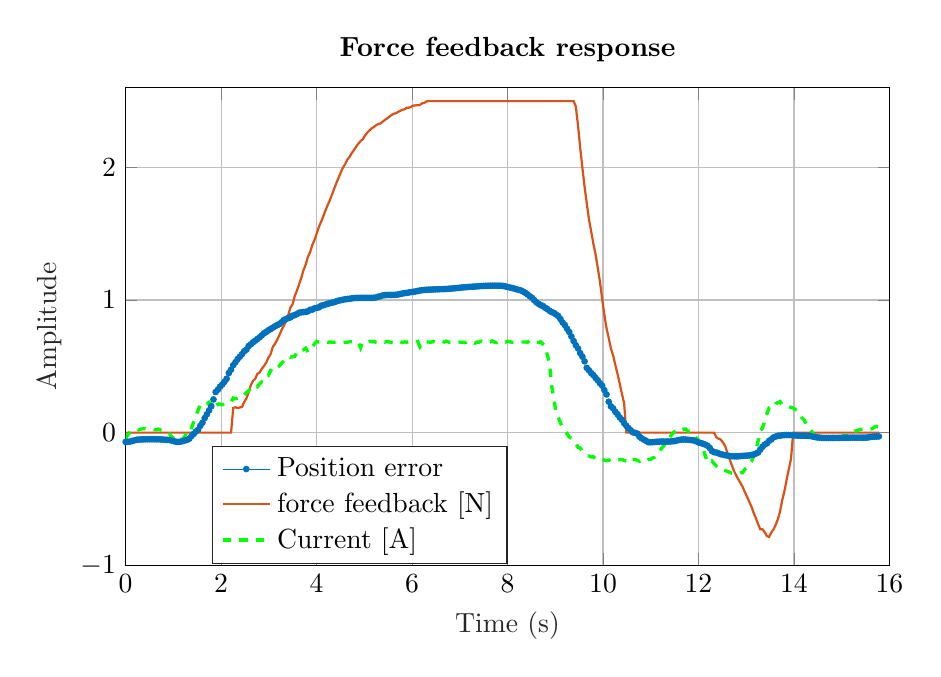
\begin{tikzpicture}

\begin{axis}[%
width=0.8\columnwidth,
height=0.5\columnwidth,
at={(2.512in,1.147in)},
scale only axis,
xmin=0,
xmax=16,
xlabel style={font=\color{white!15!black}},
xlabel={Time (s)},
ymin=-1,
ymax=2.6,
ylabel style={font=\color{white!15!black}},
ylabel={Amplitude},
axis background/.style={fill=white},
title style={font=\bfseries},
title={Force feedback response},
xmajorgrids,
ymajorgrids,
legend style={legend cell align=left, align=left, draw=white!15!black,  at={(0.5,0.25)}}
]
\addplot [color=mycolor1, draw=none, mark=*,mark size= 1, mark options={,solid, mycolor1}]
  table[row sep=crcr]{%
0	-0.069839\\
0.046	-0.0691929999999998\\
0.092	-0.0674169999999998\\
0.138	-0.0627580000000001\\
0.184	-0.0585599999999999\\
0.23	-0.053715\\
0.276	-0.052262\\
0.322	-0.0517779999999999\\
0.368	-0.0508089999999999\\
0.414	-0.050325\\
0.46	-0.0500019999999999\\
0.506	-0.0500019999999999\\
0.552	-0.0500019999999999\\
0.598	-0.0500019999999999\\
0.644	-0.050233\\
0.69	-0.0504629999999999\\
0.736	-0.0509360000000001\\
0.782	-0.0523979999999999\\
0.828	-0.0533170000000001\\
0.874	-0.0544640000000001\\
0.92	-0.0558380000000001\\
0.966	-0.059431\\
1.012	-0.0646089999999999\\
1.058	-0.069102\\
1.104	-0.070166\\
1.15	-0.0678619999999999\\
1.196	-0.0632820000000001\\
1.242	-0.0596559999999999\\
1.288	-0.054314\\
1.334	-0.045984\\
1.38	-0.0253700000000001\\
1.426	-0.00976399999999988\\
1.472	0.00805999999999996\\
1.518	0.0212249999999999\\
1.564	0.051482\\
1.61	0.0750869999999999\\
1.656	0.109672\\
1.702	0.138343\\
1.748	0.168177\\
1.794	0.199188\\
1.84	0.250473\\
1.886	0.306211\\
1.932	0.324103\\
1.978	0.347052\\
2.024	0.362787\\
2.07	0.383776\\
2.116	0.406007\\
2.162	0.449559\\
2.208	0.474824\\
2.254	0.508958\\
2.3	0.530804\\
2.346	0.554437\\
2.392	0.572537\\
2.438	0.591942\\
2.484	0.614258\\
2.53	0.625926\\
2.576	0.652916\\
2.622	0.665954\\
2.668	0.680707\\
2.714	0.6931054\\
2.76	0.7064931\\
2.806	0.7187228\\
2.852	0.7341136\\
2.898	0.7492224\\
2.944	0.7593239\\
2.99	0.7720971\\
3.036	0.7809118\\
3.082	0.7910974\\
3.128	0.8020223\\
3.174	0.81066\\
3.22	0.8186307\\
3.266	0.8319814\\
3.312	0.8492741\\
3.358	0.8558223\\
3.404	0.8646376\\
3.45	0.868742\\
3.496	0.8814436\\
3.542	0.8863328\\
3.588	0.8938385\\
3.634	0.9044656\\
3.68	0.9069801\\
3.726	0.9089659\\
3.772	0.9109976\\
3.818	0.9148639\\
3.864	0.9265554\\
3.91	0.9278963\\
3.956	0.9373217\\
4.002	0.940841\\
4.048	0.9445568\\
4.094	0.95726415\\
4.14	0.9604788\\
4.186	0.96597617\\
4.232	0.97119919\\
4.278	0.97641396\\
4.324	0.9801821\\
4.37	0.9838232\\
4.416	0.9907857\\
4.462	0.99572\\
4.508	0.9983443\\
4.554	1.0027004\\
4.6	1.0057562\\
4.646	1.0081051\\
4.692	1.0098843\\
4.738	1.0125273\\
4.784	1.0145615\\
4.83	1.015724\\
4.876	1.0164667\\
4.922	1.0164667\\
4.968	1.0164667\\
5.014	1.0164667\\
5.06	1.0164667\\
5.106	1.0164667\\
5.152	1.0164667\\
5.198	1.017048\\
5.244	1.0196638\\
5.29	1.0246052\\
5.336	1.0286748\\
5.382	1.0344887\\
5.428	1.0368141\\
5.474	1.0379768\\
5.52	1.0385582\\
5.566	1.0385582\\
5.612	1.0385582\\
5.658	1.0391396\\
5.704	1.0420462\\
5.75	1.045534\\
5.796	1.0490214\\
5.842	1.0522178\\
5.888	1.0536705\\
5.934	1.0571568\\
5.98	1.059633\\
6.026	1.062445\\
6.072	1.0644935\\
6.118	1.0679936\\
6.164	1.0718006\\
6.21	1.0739226\\
6.256	1.0760766\\
6.302	1.0773746\\
6.348	1.0781606\\
6.394	1.0786866\\
6.44	1.0796386\\
6.486	1.0806226\\
6.532	1.0811326\\
6.578	1.0815816\\
6.624	1.0821676\\
6.67	1.0826356\\
6.716	1.0836156\\
6.762	1.0849286\\
6.808	1.0862066\\
6.854	1.0874876\\
6.9	1.0889816\\
6.946	1.0904386\\
6.992	1.0921886\\
7.038	1.0943516\\
7.084	1.0958206\\
7.13	1.0971756\\
7.176	1.0983656\\
7.222	1.0995076\\
7.268	1.1005966\\
7.314	1.1015086\\
7.36	1.1031166\\
7.406	1.1045566\\
7.452	1.1057716\\
7.498	1.1059546\\
7.544	1.1072416\\
7.59	1.1076566\\
7.636	1.1080086\\
7.682	1.1083606\\
7.728	1.1083606\\
7.774	1.1082496\\
7.82	1.1082496\\
7.866	1.1078506\\
7.912	1.1055066\\
7.958	1.1023436\\
8.004	1.0977176\\
8.05	1.0940366\\
8.096	1.0909596\\
8.142	1.0861036\\
8.188	1.0816106\\
8.234	1.0766646\\
8.28	1.0723386\\
8.326	1.0637863\\
8.372	1.0543818\\
8.418	1.0428257\\
8.464	1.029448\\
8.51	1.0175659\\
8.556	1.0002029\\
8.602	0.9837055\\
8.648	0.97187785\\
8.694	0.96156563\\
8.74	0.9554396\\
8.786	0.942303\\
8.832	0.9318928\\
8.878	0.9191614\\
8.924	0.9095359\\
8.97	0.9029574\\
9.016	0.8912888\\
9.062	0.879097\\
9.108	0.8563865\\
9.154	0.8307516\\
9.2	0.8113894\\
9.246	0.7837317\\
9.292	0.7592755\\
9.338	0.725409\\
9.384	0.691096\\
9.43	0.659743\\
9.476	0.635184\\
9.522	0.599631\\
9.568	0.572746\\
9.614	0.537474\\
9.66	0.488529\\
9.706	0.470013\\
9.752	0.449131\\
9.798	0.434072\\
9.844	0.412879\\
9.89	0.394881\\
9.936	0.372667\\
9.982	0.354272\\
10.028	0.320757\\
10.074	0.287993\\
10.12	0.232964\\
10.166	0.197741\\
10.212	0.18275\\
10.258	0.156795\\
10.304	0.138484\\
10.35	0.114872\\
10.396	0.097008\\
10.442	0.071595\\
10.488	0.05155\\
10.534	0.034095\\
10.58	0.0179400000000001\\
10.626	0.002305\\
10.672	-0.00167099999999998\\
10.718	-0.00769699999999984\\
10.764	-0.030978\\
10.81	-0.0429710000000001\\
10.856	-0.053148\\
10.902	-0.0618189999999998\\
10.948	-0.0720810000000001\\
10.994	-0.0724389999999999\\
11.04	-0.0717700000000001\\
11.086	-0.0703040000000001\\
11.132	-0.068948\\
11.178	-0.0678830000000001\\
11.224	-0.067339\\
11.27	-0.067339\\
11.316	-0.067339\\
11.362	-0.0671580000000001\\
11.408	-0.0669960000000001\\
11.454	-0.065239\\
11.5	-0.063358\\
11.546	-0.0595410000000001\\
11.592	-0.054964\\
11.638	-0.052603\\
11.684	-0.051604\\
11.73	-0.0518610000000002\\
11.776	-0.053331\\
11.822	-0.0551919999999999\\
11.868	-0.0570810000000002\\
11.914	-0.059763\\
11.96	-0.0673490000000001\\
12.006	-0.075137\\
12.052	-0.0787260000000001\\
12.098	-0.084632\\
12.144	-0.090457\\
12.19	-0.099099\\
12.236	-0.115104\\
12.282	-0.138322\\
12.328	-0.147654\\
12.374	-0.150269\\
12.42	-0.156016\\
12.466	-0.1626\\
12.512	-0.166108\\
12.558	-0.169979\\
12.604	-0.172681\\
12.65	-0.176454\\
12.696	-0.177723\\
12.742	-0.178345\\
12.788	-0.179376\\
12.834	-0.178237\\
12.88	-0.176378\\
12.926	-0.175254\\
12.972	-0.174123\\
13.018	-0.172999\\
13.064	-0.171682\\
13.11	-0.167706\\
13.156	-0.164679\\
13.202	-0.157745\\
13.248	-0.1501\\
13.294	-0.127712\\
13.34	-0.106903\\
13.386	-0.0901689999999999\\
13.432	-0.0812360000000001\\
13.478	-0.0620539999999998\\
13.524	-0.0516510000000001\\
13.57	-0.035822\\
13.616	-0.029779\\
13.662	-0.0236429999999999\\
13.708	-0.0221900000000002\\
13.754	-0.0202520000000002\\
13.8	-0.0181120000000001\\
13.846	-0.018038\\
13.892	-0.018243\\
13.938	-0.0184470000000001\\
13.984	-0.019682\\
14.03	-0.0207010000000001\\
14.076	-0.0221230000000001\\
14.122	-0.023096\\
14.168	-0.023096\\
14.214	-0.023096\\
14.26	-0.0234529999999999\\
14.306	-0.024132\\
14.352	-0.0254239999999999\\
14.398	-0.0299449999999999\\
14.444	-0.033693\\
14.49	-0.0363100000000001\\
14.536	-0.0374399999999999\\
14.582	-0.0393779999999999\\
14.628	-0.039701\\
14.674	-0.0398689999999999\\
14.72	-0.0398770000000002\\
14.766	-0.039682\\
14.812	-0.039682\\
14.858	-0.039682\\
14.904	-0.039682\\
14.95	-0.039682\\
14.996	-0.0391299999999999\\
15.042	-0.0387390000000001\\
15.088	-0.0385439999999999\\
15.134	-0.038152\\
15.18	-0.0377609999999999\\
15.226	-0.0377609999999999\\
15.272	-0.0377609999999999\\
15.318	-0.0377609999999999\\
15.364	-0.0377609999999999\\
15.41	-0.0377609999999999\\
15.456	-0.0375649999999998\\
15.502	-0.0375649999999998\\
15.548	-0.036365\\
15.594	-0.0331220000000001\\
15.64	-0.030756\\
15.686	-0.0297510000000001\\
15.732	-0.02959\\
15.778	-0.028459\\
};
\addlegendentry{Position error}

\addplot [color=mycolor2, thick]
  table[row sep=crcr]{%
0	0\\
0.046	0\\
0.092	0\\
0.138	0\\
0.184	0\\
0.23	0\\
0.276	0\\
0.322	0\\
0.368	0\\
0.414	0\\
0.46	0\\
0.506	0\\
0.552	0\\
0.598	0\\
0.644	0\\
0.69	0\\
0.736	0\\
0.782	0\\
0.828	0\\
0.874	0\\
0.92	0\\
0.966	0\\
1.012	0\\
1.058	0\\
1.104	0\\
1.15	0\\
1.196	0\\
1.242	0\\
1.288	0\\
1.334	0\\
1.38	0\\
1.426	0\\
1.472	0\\
1.518	0\\
1.564	0\\
1.61	0\\
1.656	0\\
1.702	0\\
1.748	0\\
1.794	0\\
1.84	0\\
1.886	0\\
1.932	0\\
1.978	0\\
2.024	0\\
2.07	0\\
2.116	0\\
2.162	0\\
2.208	0\\
2.254	0.185892\\
2.3	0.191742\\
2.346	0.185386\\
2.392	0.189675\\
2.438	0.193986\\
2.484	0.230854\\
2.53	0.257935\\
2.576	0.303503\\
2.622	0.357063\\
2.668	0.390772\\
2.714	0.405952\\
2.76	0.443154\\
2.806	0.452801\\
2.852	0.481958\\
2.898	0.503039\\
2.944	0.527297\\
2.99	0.56528\\
3.036	0.591189\\
3.082	0.645425\\
3.128	0.670379\\
3.174	0.699748\\
3.22	0.735109\\
3.266	0.774628\\
3.312	0.805072\\
3.358	0.83938\\
3.404	0.882872\\
3.45	0.942162\\
3.496	0.967106\\
3.542	1.02907\\
3.588	1.07135\\
3.634	1.11914\\
3.68	1.16782\\
3.726	1.22586\\
3.772	1.26648\\
3.818	1.32544\\
3.864	1.36167\\
3.91	1.41453\\
3.956	1.45284\\
4.002	1.50118\\
4.048	1.55186\\
4.094	1.58921\\
4.14	1.63147\\
4.186	1.67488\\
4.232	1.71576\\
4.278	1.75288\\
4.324	1.79633\\
4.37	1.84079\\
4.416	1.88369\\
4.462	1.92324\\
4.508	1.96243\\
4.554	1.99936\\
4.6	2.02567\\
4.646	2.05945\\
4.692	2.08038\\
4.738	2.10928\\
4.784	2.13069\\
4.83	2.15696\\
4.876	2.17937\\
4.922	2.19947\\
4.968	2.21219\\
5.014	2.24018\\
5.06	2.26189\\
5.106	2.27821\\
5.152	2.29389\\
5.198	2.3042\\
5.244	2.31804\\
5.29	2.32692\\
5.336	2.33094\\
5.382	2.34414\\
5.428	2.35817\\
5.474	2.36845\\
5.52	2.38155\\
5.566	2.39363\\
5.612	2.40496\\
5.658	2.40824\\
5.704	2.41806\\
5.75	2.42631\\
5.796	2.4351\\
5.842	2.43808\\
5.888	2.45076\\
5.934	2.45048\\
5.98	2.45716\\
6.026	2.4668\\
6.072	2.46822\\
6.118	2.46973\\
6.164	2.47081\\
6.21	2.48353\\
6.256	2.48696\\
6.302	2.49787\\
6.348	2.5\\
6.394	2.5\\
6.44	2.5\\
6.486	2.5\\
6.532	2.49992\\
6.578	2.5\\
6.624	2.5\\
6.67	2.5\\
6.716	2.5\\
6.762	2.5\\
6.808	2.5\\
6.854	2.5\\
6.9	2.5\\
6.946	2.5\\
6.992	2.5\\
7.038	2.5\\
7.084	2.5\\
7.13	2.5\\
7.176	2.5\\
7.222	2.5\\
7.268	2.5\\
7.314	2.5\\
7.36	2.5\\
7.406	2.5\\
7.452	2.5\\
7.498	2.5\\
7.544	2.5\\
7.59	2.5\\
7.636	2.5\\
7.682	2.5\\
7.728	2.5\\
7.774	2.5\\
7.82	2.5\\
7.866	2.5\\
7.912	2.5\\
7.958	2.5\\
8.004	2.5\\
8.05	2.5\\
8.096	2.5\\
8.142	2.5\\
8.188	2.5\\
8.234	2.5\\
8.28	2.5\\
8.326	2.5\\
8.372	2.5\\
8.418	2.5\\
8.464	2.5\\
8.51	2.5\\
8.556	2.5\\
8.602	2.5\\
8.648	2.5\\
8.694	2.5\\
8.74	2.5\\
8.786	2.5\\
8.832	2.5\\
8.878	2.5\\
8.924	2.5\\
8.97	2.5\\
9.016	2.5\\
9.062	2.5\\
9.108	2.5\\
9.154	2.5\\
9.2	2.5\\
9.246	2.5\\
9.292	2.5\\
9.338	2.5\\
9.384	2.5\\
9.43	2.45972\\
9.476	2.31758\\
9.522	2.14825\\
9.568	1.99722\\
9.614	1.85379\\
9.66	1.72876\\
9.706	1.60717\\
9.752	1.51777\\
9.798	1.42349\\
9.844	1.34486\\
9.89	1.24209\\
9.936	1.13853\\
9.982	1.0087\\
10.028	0.888403\\
10.074	0.786921\\
10.12	0.712798\\
10.166	0.633521\\
10.212	0.58201\\
10.258	0.510575\\
10.304	0.442393\\
10.35	0.369444\\
10.396	0.293081\\
10.442	0.220909\\
10.488	0\\
10.534	0\\
10.58	0\\
10.626	0\\
10.672	0\\
10.718	0\\
10.764	0\\
10.81	0\\
10.856	0\\
10.902	0\\
10.948	0\\
10.994	0\\
11.04	0\\
11.086	0\\
11.132	0\\
11.178	0\\
11.224	0\\
11.27	0\\
11.316	0\\
11.362	0\\
11.408	0\\
11.454	0\\
11.5	0\\
11.546	0\\
11.592	0\\
11.638	0\\
11.684	0\\
11.73	0\\
11.776	0\\
11.822	0\\
11.868	0\\
11.914	0\\
11.96	0\\
12.006	0\\
12.052	0\\
12.098	0\\
12.144	0\\
12.19	0\\
12.236	0\\
12.282	0\\
12.328	0\\
12.374	-0.0349744\\
12.42	-0.046042\\
12.466	-0.0523814\\
12.512	-0.0740595\\
12.558	-0.101582\\
12.604	-0.151553\\
12.65	-0.197503\\
12.696	-0.243833\\
12.742	-0.288091\\
12.788	-0.321104\\
12.834	-0.352334\\
12.88	-0.379869\\
12.926	-0.410188\\
12.972	-0.449443\\
13.018	-0.483054\\
13.064	-0.523156\\
13.11	-0.558781\\
13.156	-0.606164\\
13.202	-0.644778\\
13.248	-0.689715\\
13.294	-0.72931\\
13.34	-0.729152\\
13.386	-0.749485\\
13.432	-0.779093\\
13.478	-0.786947\\
13.524	-0.753038\\
13.57	-0.730523\\
13.616	-0.695568\\
13.662	-0.65353\\
13.708	-0.595233\\
13.754	-0.50868\\
13.8	-0.441981\\
13.846	-0.355192\\
13.892	-0.275813\\
13.938	-0.196536\\
13.984	0\\
14.03	0\\
14.076	0\\
14.122	0\\
14.168	0\\
14.214	0\\
14.26	0\\
14.306	0\\
14.352	0\\
14.398	0\\
14.444	0\\
14.49	0\\
14.536	0\\
14.582	0\\
14.628	0\\
14.674	0\\
14.72	0\\
14.766	0\\
14.812	0\\
14.858	0\\
14.904	0\\
14.95	0\\
14.996	0\\
15.042	0\\
15.088	0\\
15.134	0\\
15.18	0\\
15.226	0\\
15.272	0\\
15.318	0\\
15.364	0\\
15.41	0\\
15.456	0\\
15.502	0\\
15.548	0\\
15.594	0\\
15.64	0\\
15.686	0\\
15.732	0\\
15.778	0\\
};
\addlegendentry{force feedback [N]}

\addplot [color=green, dashed, very thick]
  table[row sep=crcr]{%
0	-0.0462933\\
0.046	-0.0146618\\
0.092	0.00131416\\
0.138	0.0156918\\
0.184	0.0268745\\
0.23	0.0278339\\
0.276	0.0204849\\
0.322	0.027195\\
0.368	0.0300694\\
0.414	0.0303898\\
0.46	0.026556\\
0.506	0.0262356\\
0.552	0.0275135\\
0.598	0.0217628\\
0.644	0.0211239\\
0.69	0.026556\\
0.736	0.0195255\\
0.782	0.0188866\\
0.828	0.0115376\\
0.874	-0.00220108\\
0.92	-0.00891113\\
0.966	-0.0418205\\
1.012	-0.0236073\\
1.058	-0.0344715\\
1.104	-0.0450153\\
1.15	-0.0504456\\
1.196	-0.0485287\\
1.242	-0.0261631\\
1.288	0.0057869\\
1.334	0.0434895\\
1.38	0.0380573\\
1.426	0.081192\\
1.472	0.129118\\
1.518	0.168417\\
1.564	0.209953\\
1.61	0.222414\\
1.656	0.213787\\
1.702	0.216024\\
1.748	0.229124\\
1.794	0.210911\\
1.84	0.235514\\
1.886	0.200048\\
1.932	0.214746\\
1.978	0.216024\\
2.024	0.209953\\
2.07	0.219858\\
2.116	0.220497\\
2.162	0.229124\\
2.208	0.231041\\
2.254	0.261074\\
2.3	0.255003\\
2.346	0.260756\\
2.392	0.25724\\
2.438	0.278328\\
2.484	0.286955\\
2.53	0.301332\\
2.576	0.316988\\
2.622	0.329769\\
2.668	0.333603\\
2.714	0.356928\\
2.76	0.346703\\
2.806	0.368429\\
2.852	0.383766\\
2.898	0.388559\\
2.944	0.428497\\
2.99	0.431053\\
3.036	0.468117\\
3.082	0.458851\\
3.128	0.487926\\
3.174	0.492718\\
3.22	0.502623\\
3.266	0.524349\\
3.312	0.540007\\
3.358	0.557259\\
3.404	0.57675\\
3.45	0.56908\\
3.496	0.571957\\
3.542	0.575151\\
3.588	0.605825\\
3.634	0.625315\\
3.68	0.618925\\
3.726	0.624355\\
3.772	0.636816\\
3.818	0.607422\\
3.864	0.637775\\
3.91	0.646082\\
3.956	0.668768\\
4.002	0.687618\\
4.048	0.682827\\
4.094	0.686979\\
4.14	0.686022\\
4.186	0.682186\\
4.232	0.681547\\
4.278	0.683466\\
4.324	0.682507\\
4.37	0.681868\\
4.416	0.682827\\
4.462	0.684423\\
4.508	0.681547\\
4.554	0.677713\\
4.6	0.681868\\
4.646	0.680908\\
4.692	0.685062\\
4.738	0.685383\\
4.784	0.690174\\
4.83	0.685383\\
4.876	0.682507\\
4.922	0.640331\\
4.968	0.684105\\
5.014	0.683466\\
5.06	0.681229\\
5.106	0.687939\\
5.152	0.685701\\
5.198	0.688257\\
5.244	0.681229\\
5.29	0.679312\\
5.336	0.684744\\
5.382	0.688896\\
5.428	0.682827\\
5.474	0.687618\\
5.52	0.684105\\
5.566	0.67963\\
5.612	0.678034\\
5.658	0.687939\\
5.704	0.682507\\
5.75	0.686661\\
5.796	0.678991\\
5.842	0.684744\\
5.888	0.681868\\
5.934	0.685701\\
5.98	0.687939\\
6.026	0.681868\\
6.072	0.681868\\
6.118	0.687618\\
6.164	0.648638\\
6.21	0.681229\\
6.256	0.685701\\
6.302	0.684423\\
6.348	0.683784\\
6.394	0.681229\\
6.44	0.688578\\
6.486	0.681868\\
6.532	0.682186\\
6.578	0.68059\\
6.624	0.689856\\
6.67	0.683466\\
6.716	0.689856\\
6.762	0.682827\\
6.808	0.681229\\
6.854	0.680908\\
6.9	0.676756\\
6.946	0.682507\\
6.992	0.682827\\
7.038	0.680908\\
7.084	0.681229\\
7.13	0.68059\\
7.176	0.687939\\
7.222	0.678352\\
7.268	0.682827\\
7.314	0.6742\\
7.36	0.682827\\
7.406	0.682827\\
7.452	0.690174\\
7.498	0.681547\\
7.544	0.686979\\
7.59	0.685383\\
7.636	0.684744\\
7.682	0.692091\\
7.728	0.682186\\
7.774	0.678673\\
7.82	0.684744\\
7.866	0.692091\\
7.912	0.685383\\
7.958	0.682827\\
8.004	0.689535\\
8.05	0.685383\\
8.096	0.681547\\
8.142	0.683146\\
8.188	0.679951\\
8.234	0.682186\\
8.28	0.683784\\
8.326	0.683466\\
8.372	0.683784\\
8.418	0.681547\\
8.464	0.69273\\
8.51	0.680269\\
8.556	0.678034\\
8.602	0.680908\\
8.648	0.67963\\
8.694	0.685701\\
8.74	0.667809\\
8.786	0.65439\\
8.832	0.587612\\
8.878	0.522753\\
8.924	0.353092\\
8.97	0.255323\\
9.016	0.151484\\
9.062	0.117296\\
9.108	0.0735226\\
9.154	0.0380573\\
9.2	0.0124969\\
9.246	-0.00699234\\
9.292	-0.0335121\\
9.338	-0.043417\\
9.384	-0.0552387\\
9.43	-0.0792027\\
9.476	-0.110834\\
9.522	-0.115625\\
9.568	-0.141827\\
9.614	-0.156843\\
9.66	-0.174736\\
9.706	-0.176014\\
9.752	-0.183681\\
9.798	-0.182404\\
9.844	-0.197102\\
9.89	-0.203171\\
9.936	-0.201254\\
9.982	-0.195503\\
10.028	-0.207645\\
10.074	-0.211479\\
10.12	-0.208923\\
10.166	-0.199337\\
10.212	-0.202213\\
10.258	-0.196781\\
10.304	-0.204449\\
10.35	-0.202852\\
10.396	-0.202213\\
10.442	-0.209881\\
10.488	-0.214354\\
10.534	-0.191988\\
10.58	-0.20381\\
10.626	-0.202532\\
10.672	-0.203171\\
10.718	-0.208284\\
10.764	-0.21755\\
10.81	-0.212437\\
10.856	-0.201574\\
10.902	-0.212118\\
10.948	-0.202532\\
10.994	-0.201893\\
11.04	-0.190392\\
11.086	-0.184641\\
11.132	-0.171221\\
11.178	-0.150454\\
11.224	-0.119141\\
11.27	-0.100929\\
11.316	-0.0760078\\
11.362	-0.0552387\\
11.408	-0.0299988\\
11.454	-0.0085907\\
11.5	0.00866318\\
11.546	0.0224018\\
11.592	0.0313473\\
11.638	0.019846\\
11.684	0.0259171\\
11.73	0.027195\\
11.776	0.011219\\
11.822	0.00866318\\
11.868	-0.0140228\\
11.914	-0.0271225\\
11.96	-0.0399017\\
12.006	-0.058115\\
12.052	-0.0986919\\
12.098	-0.1201\\
12.144	-0.177292\\
12.19	-0.223619\\
12.236	-0.228094\\
12.282	-0.213715\\
12.328	-0.234484\\
12.374	-0.251417\\
12.42	-0.258127\\
12.466	-0.280811\\
12.512	-0.283369\\
12.558	-0.285925\\
12.604	-0.290716\\
12.65	-0.299664\\
12.696	-0.305414\\
12.742	-0.307331\\
12.788	-0.305414\\
12.834	-0.309568\\
12.88	-0.303177\\
12.926	-0.30126\\
12.972	-0.274742\\
13.018	-0.263878\\
13.064	-0.237679\\
13.11	-0.216272\\
13.156	-0.174736\\
13.202	-0.137352\\
13.248	-0.0641861\\
13.294	0.0150528\\
13.34	0.0339031\\
13.386	0.0882206\\
13.432	0.139662\\
13.478	0.188227\\
13.524	0.202286\\
13.57	0.193338\\
13.616	0.21826\\
13.662	0.226248\\
13.708	0.234556\\
13.754	0.208355\\
13.8	0.208994\\
13.846	0.203243\\
13.892	0.196533\\
13.938	0.189505\\
13.984	0.18631\\
14.03	0.17321\\
14.076	0.157873\\
14.122	0.146051\\
14.168	0.111225\\
14.214	0.0952492\\
14.26	0.0613823\\
14.306	0.0450859\\
14.352	0.0188866\\
14.398	-0.00571442\\
14.444	-0.0213718\\
14.49	-0.0296783\\
14.536	-0.0402222\\
14.582	-0.0309563\\
14.628	-0.0306377\\
14.674	-0.036068\\
14.72	-0.0379848\\
14.766	-0.0357494\\
14.812	-0.0312767\\
14.858	-0.0383053\\
14.904	-0.0303173\\
14.95	-0.0306377\\
14.996	-0.0296783\\
15.042	-0.0216904\\
15.088	-0.0216904\\
15.134	-0.0137024\\
15.18	0.000675201\\
15.226	-0.00251961\\
15.272	0.0124969\\
15.318	0.0131359\\
15.364	0.0211239\\
15.41	0.0255966\\
15.456	0.0287914\\
15.502	0.0310287\\
15.548	0.0326252\\
15.594	0.0262356\\
15.64	0.0294304\\
15.686	0.0422115\\
15.732	0.0479622\\
15.778	0.0447674\\
};
\addlegendentry{Current [A]}

\end{axis}
\end{tikzpicture}%
\caption{Friction model applied to the clamping response}
\label{fig:friction_validation}
\end{figure}

\section{Simulation}
Both the yaw and pitch model serve as a good approximation of force, but they do not adequatley capture the full dynamics of the EndoWrist.
As mentioned in section \ref{se:est}, having a better description of the general dynamics would allow for state estimates useable for state feedback control \cite{yue2004state}.

State feedback control would allow us to control the force output by the EndoWrist without having the ability to measure it during operation.
Estimated states can be used to calculate the force being applied.
Even though the current models do not allow for useable state estimates of the EndoWrist, in this section the opposite is assumed and simulated on the yaw force model.

As seen in \figref{mdle} our simulation model assumes that the EndoWrist yaw force dynamics consists of the linear system and input nonlinearities identified in chapter \ref{ch:fem}.
Our hypothesis is that full reference following capability can be added to the nonlinear system using only position error measurements and the linear model as part of a Kalman filter.

\begin{figure}[H]\label{mdle}
\centering
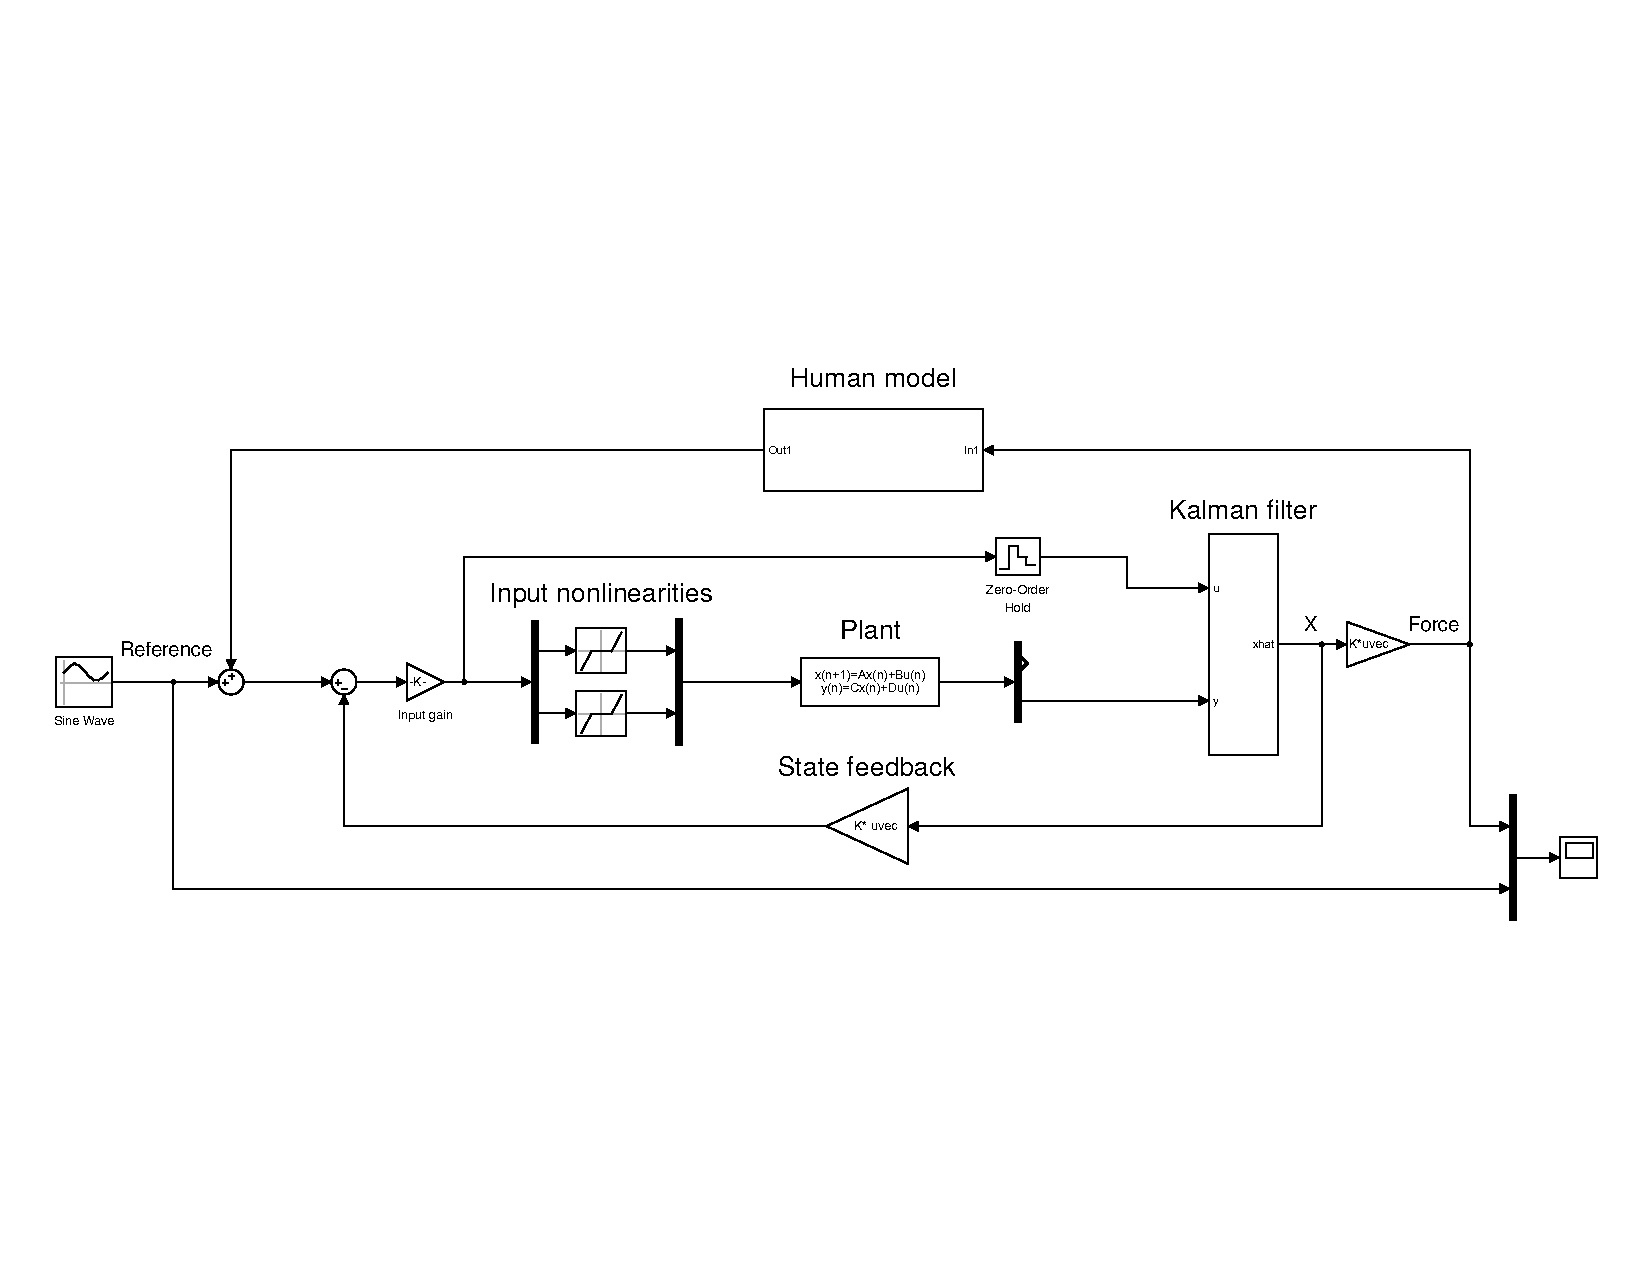
\includegraphics[width=\textwidth]{simsim.pdf}
\caption{Simulation setup.}
\end{figure}

We can see that the outer part of the system consists of a sinusoidal force reference, which is affected by oscilations from the human model. 
This represents the operators reaction to force feedback while giving a force reference.

The input nonlinearities in the system represent the effects of friction on effort and velocity, as they are the inputs to the plant (EndoWrist).
Only the position error measurement is used as an input to the kalman filter, along with the inputs.

As the Kalman filter outputs the state estimates, they are used for estimating force and providing state feedback to the input.
The estimated force is then sent to the geomagic touch, which transfers it back to the operator.

\begin{figure}[H]
\centering
\hspace{-2.5em}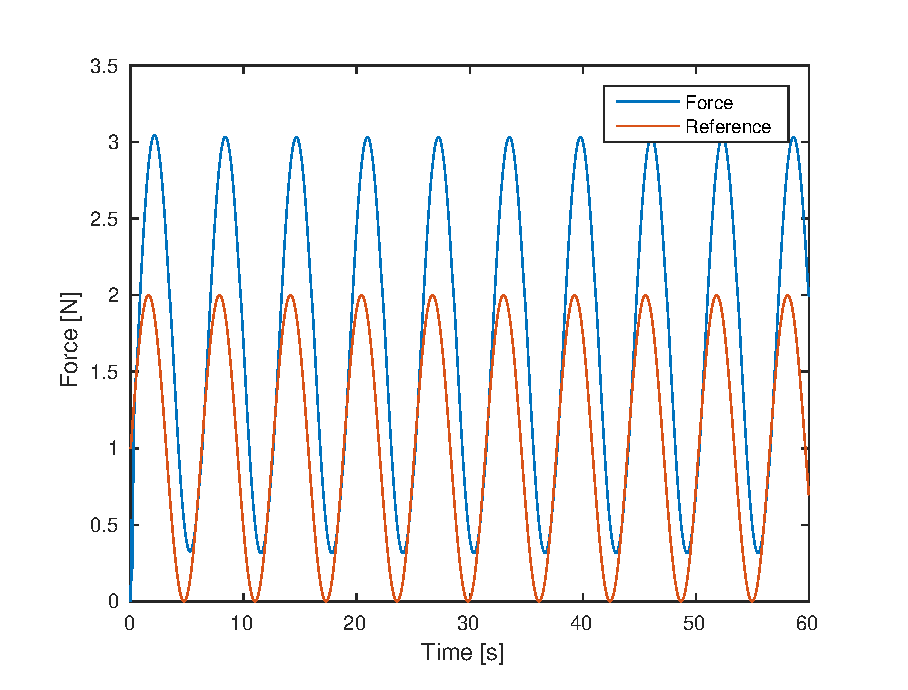
\includegraphics[width=0.7\linewidth]{reference}
\caption{Force reference following.}
\label{fig:freffl}
\end{figure}

As seen in \figref{fig:freffl} the transient behavior of the force matches that of the reference signal.
The offset and amplitude can be corrected by implementing a gain and offset to the reference.

\begin{figure}[H]
\centering
\hspace{-2.5em}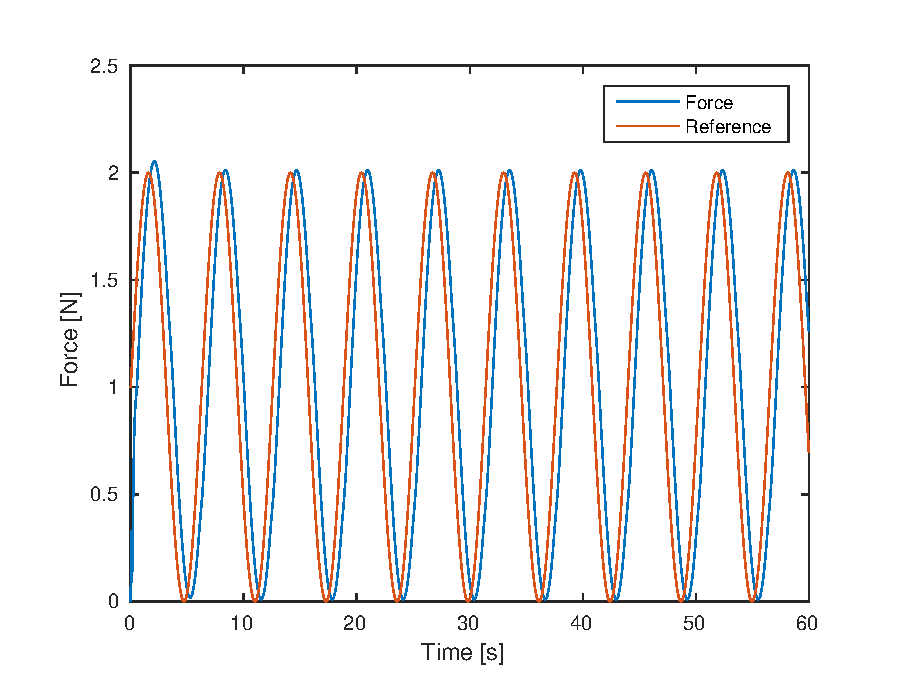
\includegraphics[width=0.7\linewidth]{reference2}
\caption{Force reference following with modified reference.}
\label{fig:freffl2}
\end{figure}

In \figref{freffl2} we can see that the modified reference indeed only leaves a delay in response of the system of about 0.3 seconds.
While this delay is significant in a surgery scenario, we believe it can be further reduced using various state space methods.
\section{Embedded control system}

It is imperative to create a controller which minimizes the effects of communication delay. Therefore the aim was to implement as much of the motion control on the embedded system as possible. The human operator  inputs the required position by moving the GT. These positions are sent as position reference to the sbRIO. 
The sbRIO has an implemented cascade position-speed-current control, see \figref{cascade_fig}, which takes care of the EndoWrist positioning tasks. The P position control that tracks the setpoint is running on the sbRIO FPGA. The FPGA sends the speed reference to the Escon controller in the form of PWM signals. The Escon controller is running the PI speed control with inner PI current control loop. The inner loops are faster than the outer loops.

The chosen controller parameters:

\begin{center}
	\begin{tabular}{ c | c | c | c }
		\hline
		Controller type & P gain & I time constant & Sampling rate \\ \hline
		Position controller & 10 & 0 & 2 kHz \\ \hline
		Speed controller & 426 & 28 ms & 5.36 kHz \\ \hline
		Position controller & 1121 & $38 \mu s$ & 53.6 kHz \\ \hline
	\end{tabular}
\end{center}

The speed and current controller parameters were calibrated automatically by ESCON Studio. The program queries the motor parameters, desired current limits and maximum acceleration values and calculates the controller parameters based on those. The EndoWrist can not handle high speeds and high acceleration, thus speed was not the main priority in tuning the position PID control. We focused on precision and avoiding overshoot. By running experiments, we decided upon a P controller of 10 for each motor. A lower gain would result in slower motion, a higher gain would result in overshoots. The EndoWrist-motor system has inherent damping in the form of friction, inertia and elasticity, thus the system is stable even without integral and differential controller. The following graph shows experiments with free-running EndoWrist. The setpoints square signals moving jumping between the limits the EndoWrist can move between. This is a movement that would never happen in normal operation.

% This file was created by matlab2tikz.
%
%The latest updates can be retrieved from
%  http://www.mathworks.com/matlabcentral/fileexchange/22022-matlab2tikz-matlab2tikz
%where you can also make suggestions and rate matlab2tikz.
%
\definecolor{mycolor1}{rgb}{0.00000,0.44700,0.74100}%
\definecolor{mycolor2}{rgb}{0.85000,0.32500,0.09800}%
%
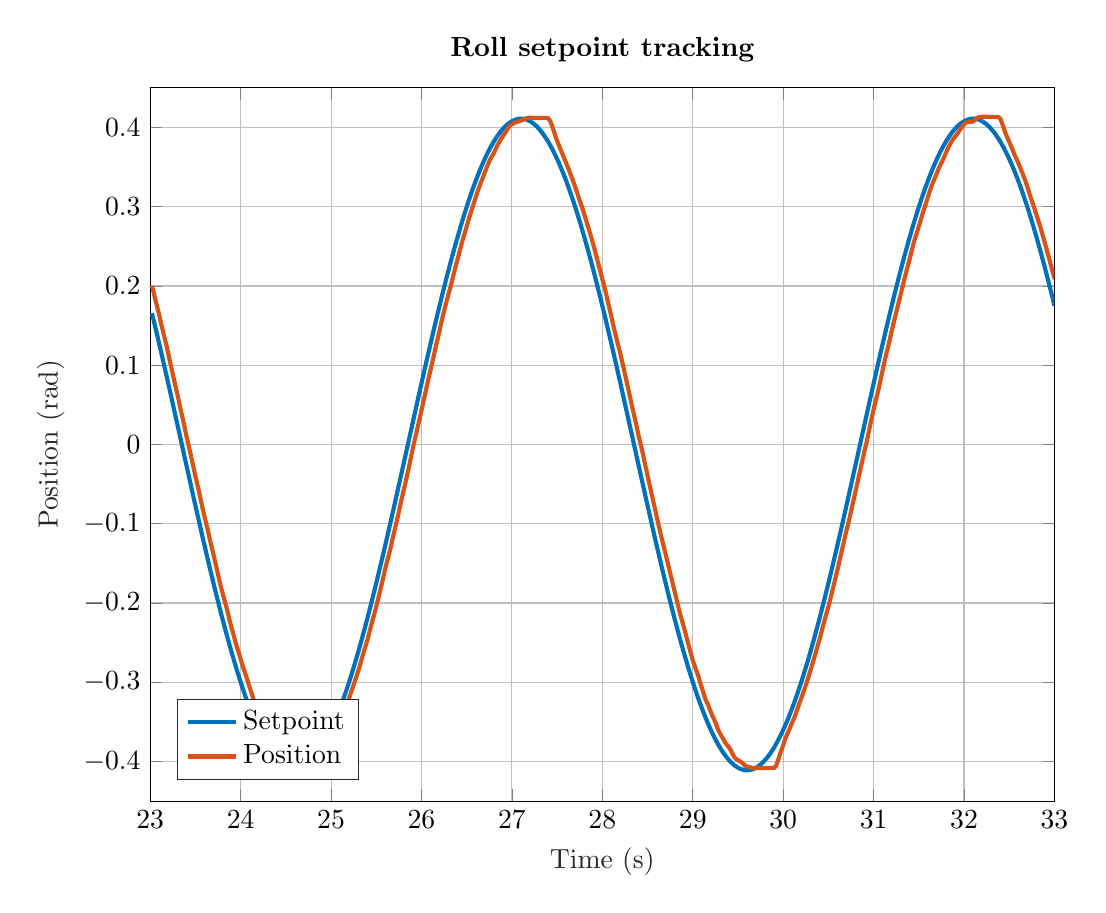
\begin{tikzpicture}

\begin{axis}[%
width=4.521in,
height=3.566in,
at={(0.758in,0.481in)},
scale only axis,
xmin=23,
xmax=33,
xlabel style={font=\color{white!15!black}},
xlabel={Time (s)},
ymin=-0.45,
ymax=0.45,
ylabel style={font=\color{white!15!black}},
ylabel={Position (rad)},
axis background/.style={fill=white},
title style={font=\bfseries},
title={Roll setpoint tracking},
xmajorgrids,
ymajorgrids,
legend style={at={(0.03,0.03)}, anchor=south west, legend cell align=left, align=left, draw=white!15!black}
]
\addplot [color=mycolor1, line width=1.5pt]
  table[row sep=crcr]{%
23.0191555	0.165668769531251\\
23.0791626	0.136850136718749\\
23.11917114	0.117195410156249\\
23.19929695	0.0770482421875016\\
23.3391819	0.00516695312499849\\
23.47919846	-0.0668738281249972\\
23.57920647	-0.117195410156249\\
23.65921402	-0.15615916015625\\
23.71923447	-0.1843680859375\\
23.77923203	-0.211529414062497\\
23.83923912	-0.237488769531247\\
23.87924385	-0.254054121093752\\
23.93925476	-0.277686171874997\\
23.9792614	-0.292572246093748\\
24.01925659	-0.306719218749997\\
24.05926514	-0.32009140625\\
24.09938622	-0.332655000000003\\
24.1392746	-0.344378320312501\\
24.17927551	-0.35523166015625\\
24.21928978	-0.36518767578125\\
24.25928879	-0.374221191406249\\
24.2994175	-0.382309394531248\\
24.33930206	-0.38943185546875\\
24.37930679	-0.395570585937499\\
24.41931152	-0.400710058593752\\
24.45931435	-0.404837304687497\\
24.49943924	-0.407941894531248\\
24.53932953	-0.410015976562498\\
24.57933235	-0.41105435546875\\
24.61933899	-0.41105435546875\\
24.65933609	-0.410015976562498\\
24.69947052	-0.407941894531248\\
24.73935127	-0.404837304687497\\
24.77935219	-0.400710058593752\\
24.81936455	-0.395570585937499\\
24.85939026	-0.38943185546875\\
24.89950562	-0.382309394531248\\
24.93938637	-0.374221191406249\\
24.97940445	-0.36518767578125\\
25.01939392	-0.35523166015625\\
25.05941391	-0.344378320312501\\
25.09952736	-0.332655000000003\\
25.13941765	-0.32009140625\\
25.17942429	-0.306719218749997\\
25.21941948	-0.292572246093748\\
25.2595253	-0.277686171874997\\
25.29954147	-0.262098671875002\\
25.33945274	-0.245849082031249\\
25.37944412	-0.228978476562503\\
25.41944885	-0.211529414062497\\
25.45945358	-0.193546015625003\\
25.51947403	-0.165668769531251\\
25.57947159	-0.136850136718749\\
25.61948204	-0.117195410156249\\
25.69965935	-0.0770482421875016\\
25.89969635	0.0258184765624989\\
25.95955086	0.0566571875000008\\
26.03957939	0.0972446484375027\\
26.09970474	0.127062910156248\\
26.13957214	0.146550937500002\\
26.17958832	0.165668769531251\\
26.23957825	0.193546015625003\\
26.27958679	0.211529414062497\\
26.33958435	0.237488769531247\\
26.37959862	0.254054121093752\\
26.43959999	0.277686171874997\\
26.47961998	0.292572246093748\\
26.51965904	0.306719218749997\\
26.559618	0.32009140625\\
26.59978867	0.332655000000003\\
26.63961983	0.344378320312501\\
26.67969131	0.35523166015625\\
26.71968079	0.36518767578125\\
26.7596817	0.374221191406249\\
26.79981041	0.382309394531248\\
26.83969688	0.38943185546875\\
26.8796978	0.395570585937499\\
26.91968918	0.400710058593752\\
26.95970345	0.404837304687497\\
26.9998188	0.407941894531248\\
27.03972244	0.410015976562498\\
27.07970428	0.41105435546875\\
27.11972046	0.41105435546875\\
27.15972137	0.410015976562498\\
27.19987488	0.407941894531248\\
27.23973846	0.404837304687497\\
27.27972794	0.400710058593752\\
27.31974983	0.395570585937499\\
27.3597641	0.38943185546875\\
27.39987946	0.382309394531248\\
27.43976212	0.374221191406249\\
27.47976685	0.36518767578125\\
27.51978683	0.35523166015625\\
27.55976677	0.344378320312501\\
27.59990501	0.332655000000003\\
27.63977814	0.32009140625\\
27.67980003	0.306719218749997\\
27.71977997	0.292572246093748\\
27.75979042	0.277686171874997\\
27.79992867	0.262098671875002\\
27.83981323	0.245849082031249\\
27.87981415	0.228978476562503\\
27.91983032	0.211529414062497\\
27.97982025	0.1843680859375\\
28.01981544	0.165668769531251\\
28.07985115	0.136850136718749\\
28.11987686	0.117195410156249\\
28.19997215	0.0770482421875016\\
28.31985855	0.0154976171874992\\
28.47991753	-0.0668738281249972\\
28.57987976	-0.117195410156249\\
28.65989304	-0.15615916015625\\
28.71993256	-0.1843680859375\\
28.75995255	-0.202601699218746\\
28.80004501	-0.220323515624997\\
28.8399334	-0.237488769531247\\
28.87992287	-0.254054121093752\\
28.93993759	-0.277686171874997\\
28.97994614	-0.292572246093748\\
29.01994705	-0.306719218749997\\
29.05997849	-0.32009140625\\
29.10009575	-0.332655000000003\\
29.13996696	-0.344378320312501\\
29.17998505	-0.35523166015625\\
29.21994209	-0.36518767578125\\
29.25997353	-0.374221191406249\\
29.30012321	-0.382309394531248\\
29.34000587	-0.38943185546875\\
29.3800087	-0.395570585937499\\
29.41999435	-0.400710058593752\\
29.46001816	-0.404837304687497\\
29.50014114	-0.407941894531248\\
29.54003143	-0.410015976562498\\
29.58001518	-0.41105435546875\\
29.62005615	-0.41105435546875\\
29.66002274	-0.410015976562498\\
29.70015717	-0.407941894531248\\
29.74006462	-0.404837304687497\\
29.78003311	-0.400710058593752\\
29.82004356	-0.395570585937499\\
29.86007118	-0.38943185546875\\
29.90019608	-0.382309394531248\\
29.94006538	-0.374221191406249\\
29.98004532	-0.36518767578125\\
30.02007484	-0.35523166015625\\
30.06008911	-0.344378320312501\\
30.10021591	-0.332655000000003\\
30.14009857	-0.32009140625\\
30.18009949	-0.306719218749997\\
30.22017097	-0.292572246093748\\
30.26011658	-0.277686171874997\\
30.30026627	-0.262098671875002\\
30.34012604	-0.245849082031249\\
30.40029907	-0.220323515624997\\
30.4601326	-0.193546015625003\\
30.52017593	-0.165668769531251\\
30.58013344	-0.136850136718749\\
30.62013245	-0.117195410156249\\
30.70029259	-0.0770482421875016\\
30.84021378	-0.00516695312499849\\
30.980196	0.0668738281249972\\
31.08020401	0.117195410156249\\
31.1602459	0.15615916015625\\
31.22019577	0.1843680859375\\
31.28022957	0.211529414062497\\
31.34022331	0.237488769531247\\
31.38021278	0.254054121093752\\
31.44024277	0.277686171874997\\
31.48025322	0.292572246093748\\
31.520298	0.306719218749997\\
31.56042099	0.32009140625\\
31.60041428	0.332655000000003\\
31.64028549	0.344378320312501\\
31.68028259	0.35523166015625\\
31.72029877	0.36518767578125\\
31.76030731	0.374221191406249\\
31.80044556	0.382309394531248\\
31.84035492	0.38943185546875\\
31.88029289	0.395570585937499\\
31.92034912	0.400710058593752\\
31.96029282	0.404837304687497\\
32.00043488	0.407941894531248\\
32.04032898	0.410015976562498\\
32.08035278	0.41105435546875\\
32.12031555	0.41105435546875\\
32.16034317	0.410015976562498\\
32.20049286	0.407941894531248\\
32.24038315	0.404837304687497\\
32.28037262	0.400710058593752\\
32.32038116	0.395570585937499\\
32.36040878	0.38943185546875\\
32.40048218	0.382309394531248\\
32.44039536	0.374221191406249\\
32.48039627	0.36518767578125\\
32.5204277	0.35523166015625\\
32.56040192	0.344378320312501\\
32.60052109	0.332655000000003\\
32.64037704	0.32009140625\\
32.68041992	0.306719218749997\\
32.72045135	0.292572246093748\\
32.7604332	0.277686171874997\\
32.8005867	0.262098671875002\\
32.86040115	0.237488769531247\\
32.90053558	0.220323515624997\\
32.96042633	0.193546015625003\\
33.00058746	0.175073710937497\\
};
\addlegendentry{Setpoint}

\addplot [color=mycolor2, line width=1.5pt]
  table[row sep=crcr]{%
23.0191555	0.200063183593748\\
23.03915405	0.191505195312502\\
23.05915833	0.181332500000003\\
23.0992794	0.163247695312499\\
23.11917114	0.153074980468752\\
23.15916443	0.134182812500001\\
23.17917252	0.125140410156249\\
23.19929695	0.114806230468751\\
23.21917725	0.104149121093748\\
23.27918243	0.0737924804687466\\
23.29930305	0.0639427148437477\\
23.31919098	0.0529626562500027\\
23.3391819	0.0426284765624985\\
23.35918236	0.0327787109374995\\
23.37919235	0.0222830664062528\\
23.39931488	0.0111415234375016\\
23.41919327	0.00161470703125133\\
23.43920135	-0.00839652343749719\\
23.4993248	-0.0398834570312516\\
23.53920555	-0.0595829882812495\\
23.57920647	-0.0807357421874997\\
23.63921356	-0.1093162109375\\
23.65921402	-0.119650371093748\\
23.69934082	-0.138865488281247\\
23.77923203	-0.178748945312499\\
23.83923912	-0.203777031249999\\
23.87924385	-0.222507714843751\\
23.89936638	-0.231227187499996\\
23.91924667	-0.239462226562502\\
23.93925476	-0.248181699218748\\
23.95925522	-0.255770859374998\\
23.9792614	-0.26287560546875\\
24.01925659	-0.278215390625\\
24.05926514	-0.291940468749999\\
24.1392746	-0.32052091796875\\
24.21928978	-0.343934277343749\\
24.23929024	-0.34910138671875\\
24.25928879	-0.354914375\\
24.27929878	-0.361211738281249\\
24.2994175	-0.364925605468748\\
24.33930206	-0.374129453125001\\
24.35929871	-0.377843300781251\\
24.39942551	-0.383979238281249\\
24.4393177	-0.39156837890625\\
24.45931435	-0.394636367187502\\
24.47932053	-0.396896933593752\\
24.53932953	-0.399641953124998\\
24.55933571	-0.402225507812503\\
24.57933235	-0.405293457031249\\
24.59946823	-0.4069081640625\\
24.61933899	-0.407876992187497\\
24.67933464	-0.408038476562503\\
24.87937546	-0.407715527343747\\
24.89950562	-0.407554062499997\\
24.9193821	-0.404001679687497\\
24.9593811	-0.392214277343747\\
24.99950981	-0.379296582031252\\
25.03940964	-0.367024707031248\\
25.05941391	-0.362180546875003\\
25.07941818	-0.356851992187501\\
25.11941338	-0.345064589843751\\
25.13941765	-0.338282792968748\\
25.15943146	-0.332469824218748\\
25.17942429	-0.326172421875\\
25.19954681	-0.320197988281251\\
25.21941948	-0.313093222656249\\
25.23942566	-0.306795839843751\\
25.27942657	-0.293232246093751\\
25.31944466	-0.278861289062498\\
25.33945274	-0.270303281250001\\
25.37944412	-0.254963496093751\\
25.39957237	-0.2475358203125\\
25.41944885	-0.238977812500003\\
25.43946648	-0.229773945312502\\
25.47947884	-0.213465312499999\\
25.49957657	-0.204584394531253\\
25.55951691	-0.17648833984375\\
25.57947159	-0.166800058593751\\
25.59960938	-0.156465878906253\\
25.61948204	-0.147423476562501\\
25.63947678	-0.139349902343753\\
25.65950775	-0.129984570312502\\
25.67949295	-0.119327421874999\\
25.71951675	-0.100112324218749\\
25.7395134	-0.0904240429687491\\
25.77954102	-0.0691098046874998\\
25.81952286	-0.0498946875000001\\
25.83953857	-0.0392375781249967\\
25.85951996	-0.0295492773437473\\
25.89969635	-0.00710474609375211\\
25.97954559	0.0327787109374995\\
26.07955933	0.0841266601562509\\
26.11956024	0.1035032421875\\
26.13957214	0.113998886718747\\
26.17958832	0.133536933593753\\
26.19974518	0.143709628906251\\
26.21959496	0.154366757812497\\
26.23957825	0.163893574218747\\
26.29973793	0.190536367187498\\
26.31958199	0.198125527343748\\
26.37959862	0.225737148437503\\
26.39978218	0.234133671875\\
26.43959999	0.251572617187499\\
26.45960236	0.259969121093754\\
26.47961998	0.267235332031248\\
26.49975395	0.274985937499999\\
26.51965904	0.283059550781253\\
26.53966522	0.290648691406247\\
26.61962128	0.318906191406249\\
26.65966988	0.331500976562502\\
26.67969131	0.336829550781253\\
26.69979858	0.342803984375003\\
26.71968079	0.3492628515625\\
26.7596817	0.359758496093747\\
26.77966881	0.363795292968753\\
26.79981041	0.367509121093747\\
26.81968689	0.372676230468748\\
26.83969688	0.377520371093752\\
26.8796978	0.3855939453125\\
26.91968918	0.392214277343747\\
26.95970345	0.399641953124998\\
26.97970009	0.402548437500002\\
27.01970673	0.405293457031249\\
27.05970955	0.407231132812498\\
27.07970428	0.407715527343747\\
27.09983826	0.40884583984375\\
27.11972046	0.409330234374998\\
27.1397171	0.410299082031251\\
27.15972137	0.411752324218753\\
27.17972946	0.412236757812501\\
27.37975121	0.412075234375003\\
27.39987946	0.411752324218753\\
27.41974258	0.408684375\\
27.43976212	0.403355800781249\\
27.45976257	0.396896933593752\\
27.47976685	0.389469238281251\\
27.49986458	0.383010390625003\\
27.57977867	0.360565839843751\\
27.59990501	0.35523728515625\\
27.63977814	0.34361134765625\\
27.67980003	0.331662441406252\\
27.71977997	0.318260312500001\\
27.73979187	0.311155566406249\\
27.77978325	0.298076406249997\\
27.87981415	0.260453535156252\\
27.89992714	0.252379941406247\\
27.93980408	0.235263964843753\\
27.99995804	0.208459687500003\\
28.01981544	0.200224667968747\\
28.03981781	0.191343730468752\\
28.05982971	0.181009550781248\\
28.09995842	0.16131001953125\\
28.11987686	0.151137304687502\\
28.13983154	0.141449023437502\\
28.19997215	0.113998886718747\\
28.23985672	0.0941378906249994\\
28.27983856	0.073469531249998\\
28.3000145	0.0634583007812495\\
28.31985855	0.052639707031247\\
28.37986183	0.022767480468751\\
28.40002632	0.0114644726562503\\
28.41988564	0.00226060546874862\\
28.43987274	-0.00742769531250076\\
28.45988464	-0.0184077539062528\\
28.51988983	-0.049571757812501\\
28.57987976	-0.080251347656251\\
28.61990929	-0.100596738281247\\
28.65989304	-0.119973320312504\\
28.67989922	-0.129015722656249\\
28.8399334	-0.204584394531253\\
28.85992241	-0.213626796874998\\
28.91993523	-0.23817044921875\\
28.93993759	-0.247374316406251\\
29.00005722	-0.272402421875\\
29.01994705	-0.279184199218747\\
29.05997849	-0.29177900390625\\
29.0799942	-0.299691113281249\\
29.13996696	-0.321489765625003\\
29.15997696	-0.32633388671875\\
29.17998505	-0.331662441406252\\
29.20013809	-0.33779837890625\\
29.21994209	-0.343126933593751\\
29.23999405	-0.347809609374998\\
29.25997353	-0.353622578124998\\
29.27997208	-0.359919960937503\\
29.30012321	-0.36444119140625\\
29.34000587	-0.372191796875001\\
29.36000061	-0.376551523437499\\
29.3800087	-0.379619472656252\\
29.40013885	-0.38188009765625\\
29.41999435	-0.385916874999999\\
29.46001816	-0.394797792968753\\
29.48002243	-0.3970584375\\
29.5200119	-0.399641953124998\\
29.54003143	-0.4010951953125\\
29.58001518	-0.405454921874998\\
29.60014915	-0.406423750000002\\
29.62005615	-0.406746699218751\\
29.66002274	-0.408361425781251\\
29.90019608	-0.408038476562503\\
29.92011642	-0.405939355468753\\
29.94006538	-0.399480488281249\\
29.98004532	-0.38575541015625\\
30.00018692	-0.379296582031252\\
30.02007484	-0.372514746093749\\
30.0401001	-0.366701777343749\\
30.06008911	-0.361857617187503\\
30.08009148	-0.356044648437504\\
30.12007904	-0.345710468749999\\
30.14009857	-0.33973603515625\\
30.18009949	-0.326010957031251\\
30.20022011	-0.320359453125\\
30.26011658	-0.300498437500003\\
30.32013321	-0.27837685546875\\
30.34012604	-0.270303281250001\\
30.36011124	-0.262714140625\\
30.38015175	-0.254479082031253\\
30.40029907	-0.246728457031253\\
30.42012215	-0.238331933593749\\
30.44019699	-0.229128046874997\\
30.50025749	-0.204422910156246\\
30.52017593	-0.19570345703125\\
30.60030365	-0.158242070312497\\
30.62013245	-0.148069355468749\\
30.70029259	-0.108347363281247\\
30.7202034	-0.0994664453125012\\
30.74013329	-0.0897781640625013\\
30.80030251	-0.0589370898437522\\
30.82019997	-0.0489258593749966\\
30.84021378	-0.0381072656250012\\
30.8602047	-0.0284189843750013\\
30.90029144	-0.00758916015625033\\
30.92017746	0.00161470703125133\\
30.94021988	0.0122718359374971\\
30.96017838	0.0234133593749988\\
31.00031853	0.0445661328124984\\
31.02017975	0.0539314843749992\\
31.04024887	0.0626509375000026\\
31.06018448	0.072339238281252\\
31.10031509	0.0941378906249994\\
31.14019394	0.114321816406253\\
31.1602459	0.123202753906249\\
31.20035934	0.143225214843753\\
31.22019577	0.152752031250003\\
31.32023621	0.198932871093753\\
31.34022331	0.208459687500003\\
31.38021278	0.226221562500001\\
31.40035629	0.234779550781248\\
31.42024994	0.24366048828125\\
31.44024277	0.253025820312502\\
31.46025085	0.260776464843751\\
31.48025322	0.267719765625003\\
31.50040054	0.275631835937503\\
31.54026985	0.290648691406247\\
31.5802803	0.304696699218752\\
31.60041428	0.312285878906252\\
31.62028503	0.319390644531254\\
31.64028549	0.325849492187501\\
31.66029358	0.331662441406252\\
31.70036697	0.342319570312497\\
31.72029877	0.348294042968753\\
31.74024773	0.35329962890625\\
31.76030731	0.357659355468748\\
31.78029251	0.362987929687499\\
31.80044556	0.367993554687502\\
31.82031822	0.373322109375003\\
31.8602562	0.3820415625\\
31.88029289	0.3855939453125\\
31.90040207	0.388177480468748\\
31.94027901	0.394313398437497\\
31.96029282	0.398188710937497\\
31.98027229	0.401256699218749\\
32.02036285	0.406100800781253\\
32.04032898	0.406746699218751\\
32.08035278	0.4069081640625\\
32.10045242	0.407715527343747\\
32.12031555	0.409330234374998\\
32.14030457	0.411752324218753\\
32.16034317	0.41288259765625\\
32.20049286	0.413528496093747\\
32.36040878	0.413367031249997\\
32.38039017	0.413044121093748\\
32.40048218	0.411267890624998\\
32.42037964	0.405616386718748\\
32.46037674	0.392214277343747\\
32.54035187	0.371222968749997\\
32.56040192	0.365248535156248\\
32.60052109	0.35523728515625\\
32.64037704	0.343934277343749\\
32.68041992	0.331985390625\\
32.70054245	0.325203613281253\\
32.74040604	0.310671171875001\\
32.78042221	0.297269023437501\\
32.84041977	0.275793320312502\\
32.90053558	0.251734082031248\\
32.98042679	0.217825058593753\\
33.00058746	0.208782636718752\\
};
\addlegendentry{Position}

\end{axis}
\end{tikzpicture}%

\begin{figure}[h] \label{ fig7} \begin{minipage}[b]{0.50\linewidth}\centering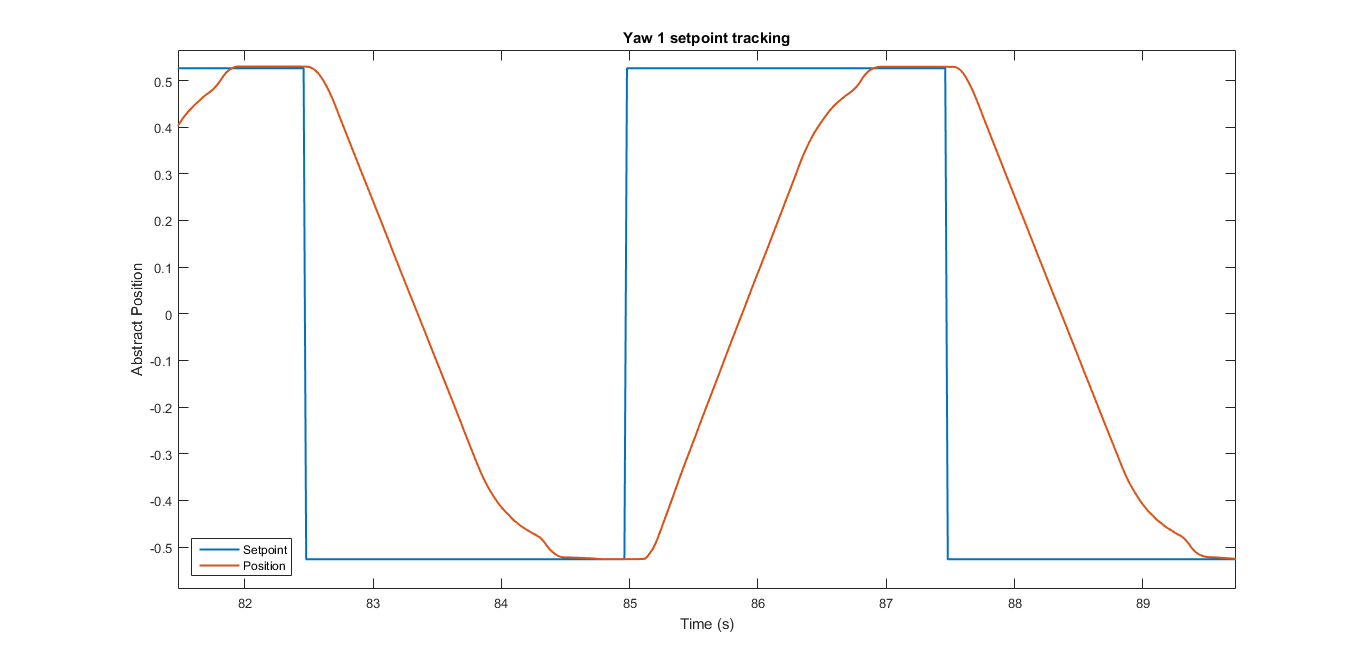
\includegraphics[width=0.70\linewidth]{extreme_yaw1.png} \caption{} \end{minipage} \begin{minipage}[b]{0.50\linewidth}\centering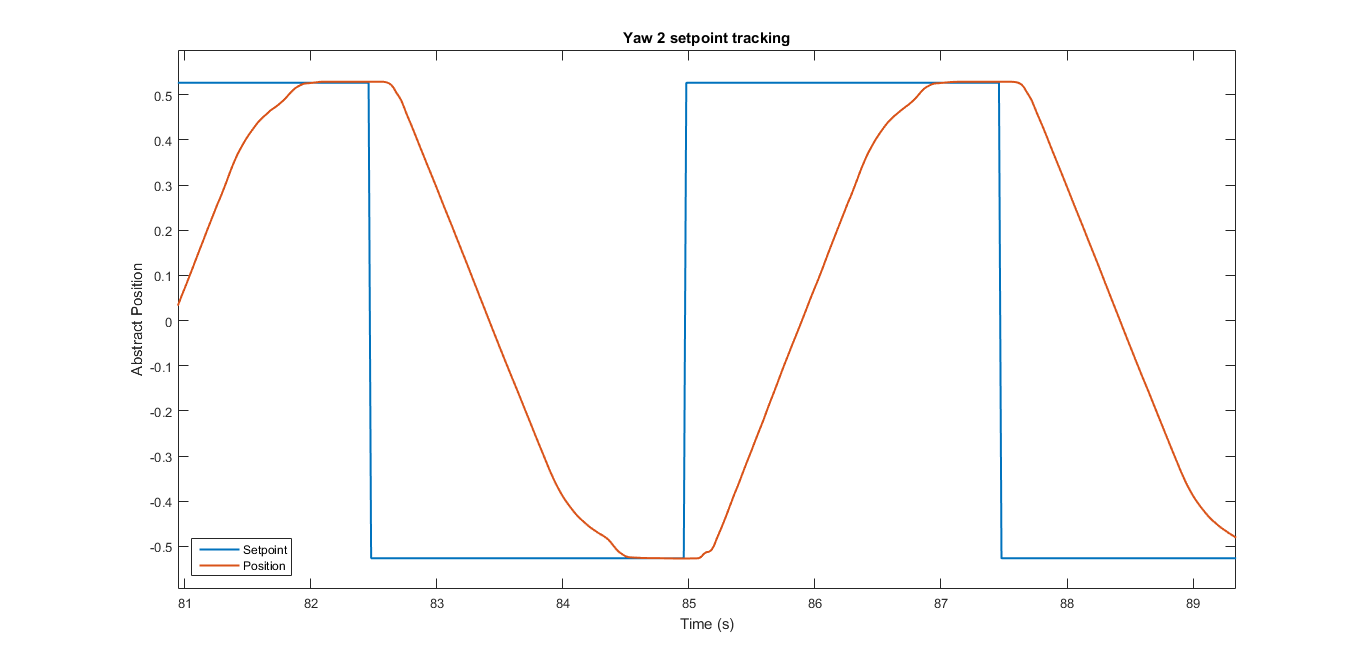
\includegraphics[width=0.70\linewidth]{extreme_yaw2.png} \caption{} \end{minipage} \begin{minipage}[b]{0.50\linewidth}\centering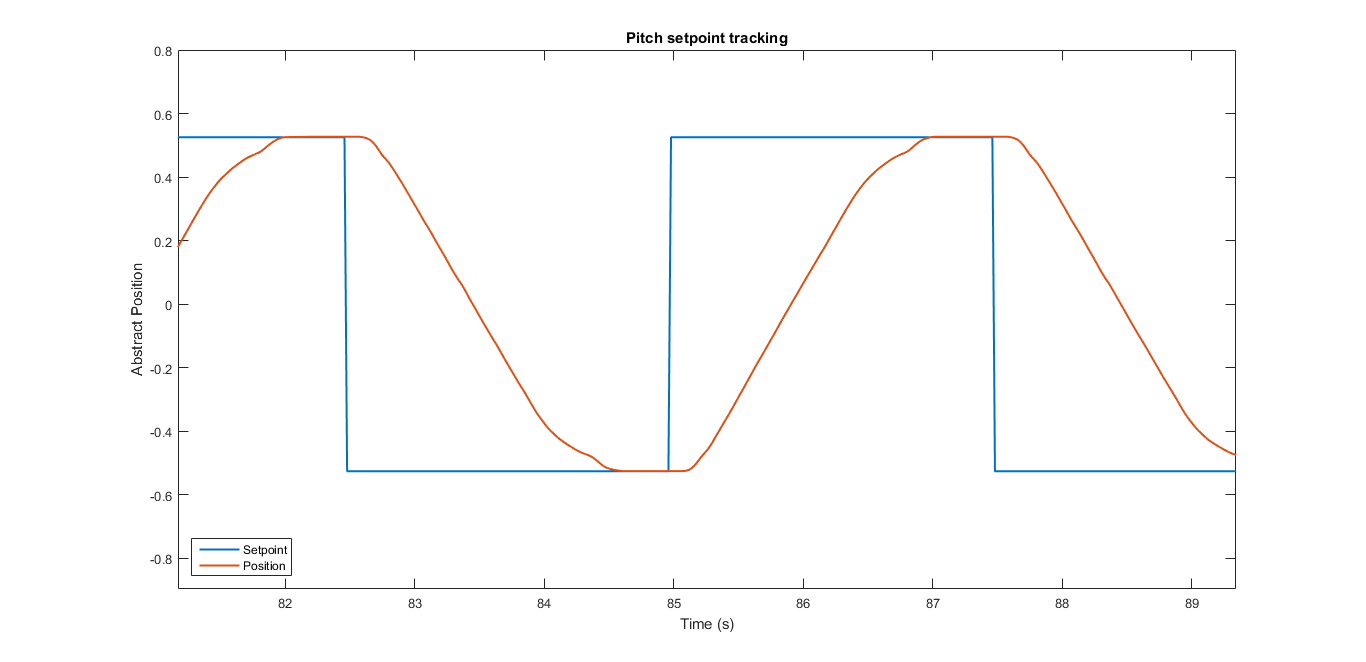
\includegraphics[width=0.70\linewidth]{extreme_pitch.png} \caption{} \end{minipage}\hfill \begin{minipage}[b]{0.50\linewidth}\centering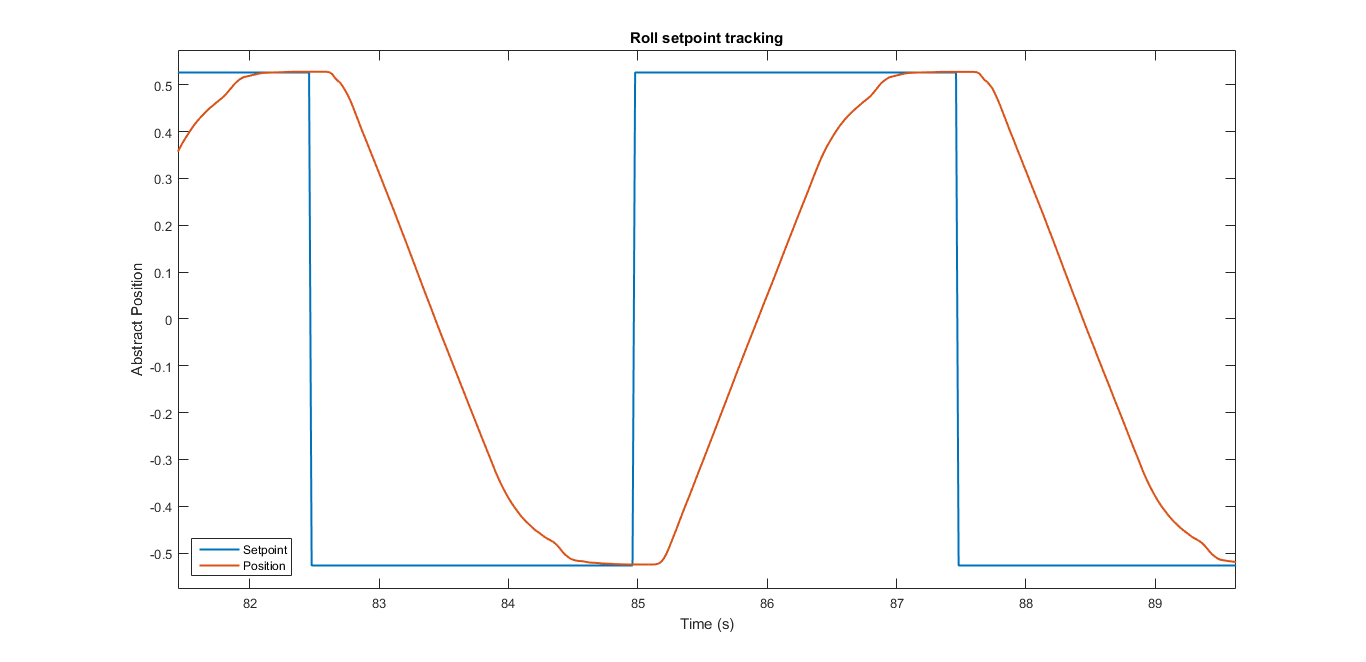
\includegraphics[width=0.70\linewidth]{extreme_roll.png} \caption{} \end{minipage} \end{figure}

\begin{figure}[h] \label{ fig7} \begin{minipage}[b]{0.50\linewidth}\centering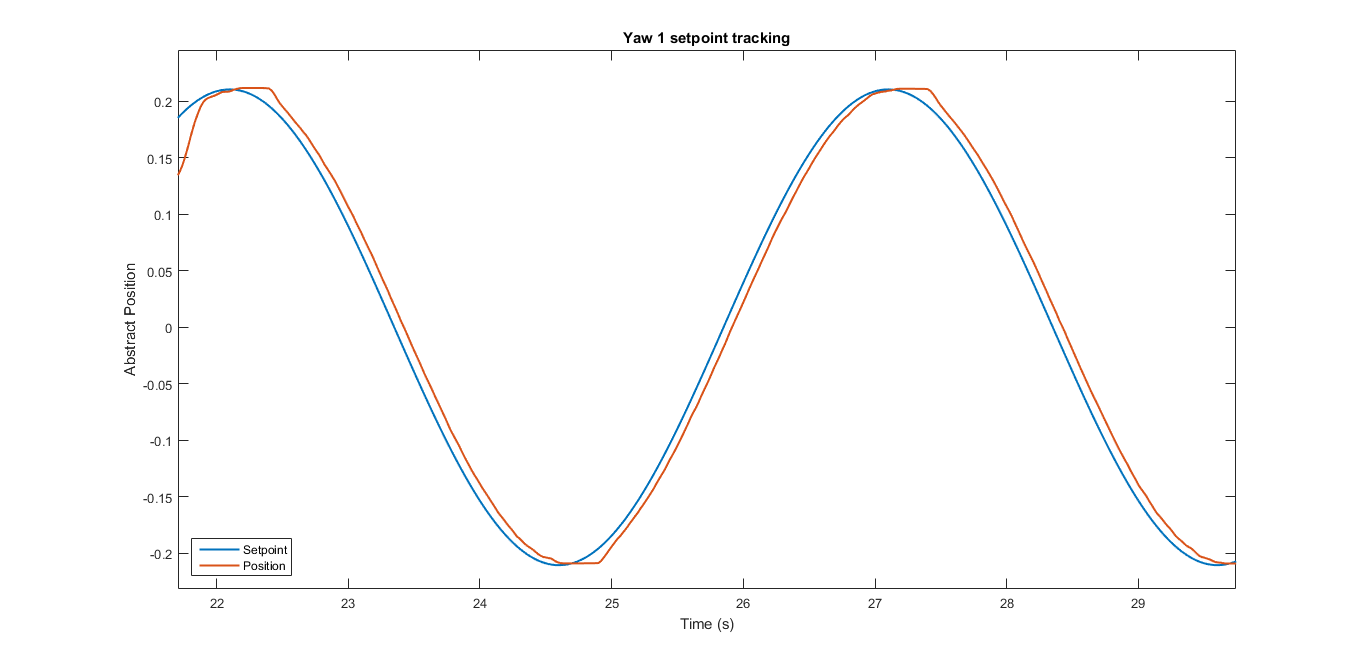
\includegraphics[width=0.70\linewidth]{mild_yaw1.png} \caption{The yaw setpoint tracking lag in this case is 50 ms} \end{minipage} \begin{minipage}[b]{0.50\linewidth}\centering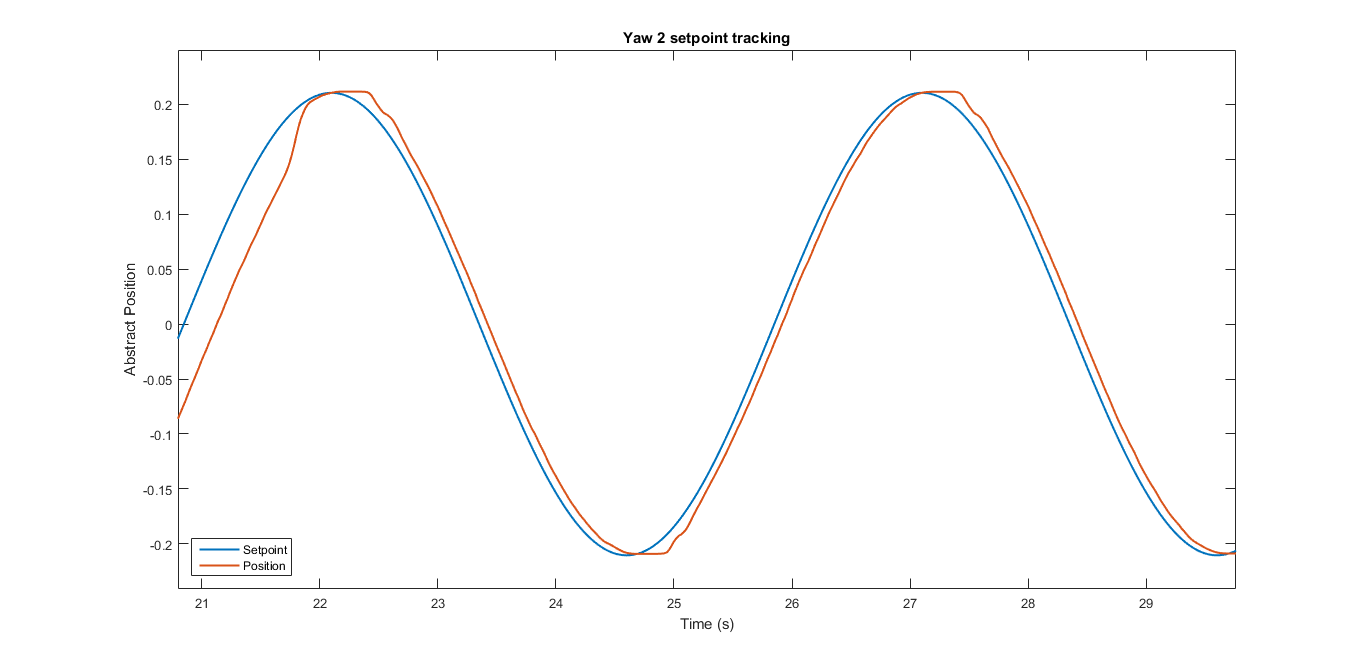
\includegraphics[width=0.70\linewidth]{mild_yaw2.png} \caption{} \end{minipage} \begin{minipage}[b]{0.50\linewidth}\centering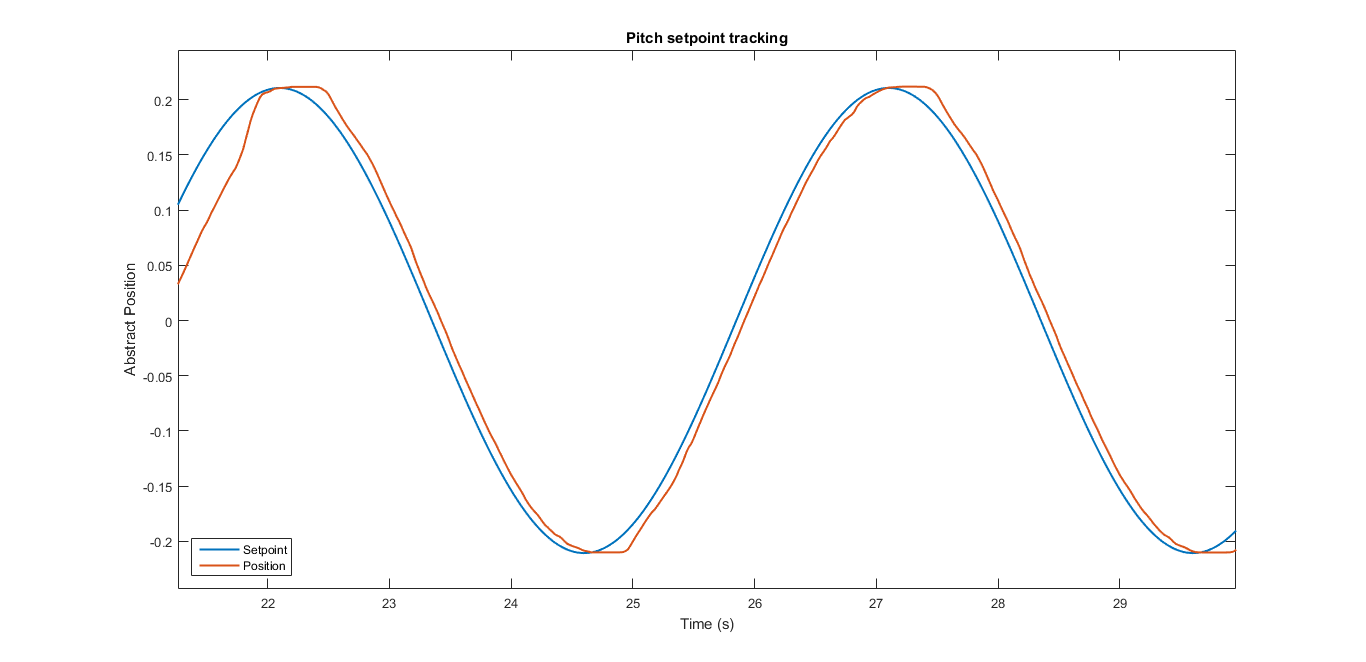
\includegraphics[width=0.70\linewidth]{mild_pitch.png} \caption{} \end{minipage}\hfill \begin{minipage}[b]{0.50\linewidth}\centering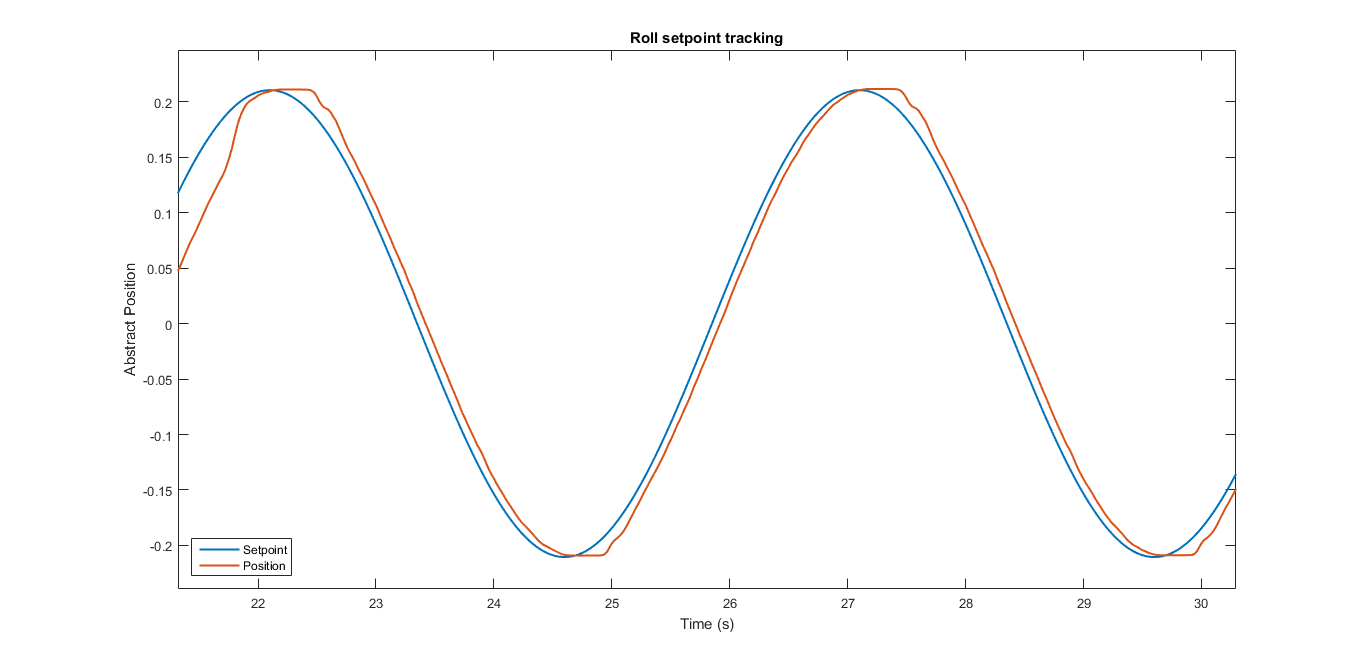
\includegraphics[width=0.70\linewidth]{mild_roll.png} \caption{} \end{minipage} \end{figure}


The following graph shows measurements with sinusoidal setpoint signals. This is much more similar to normal operations, where instead of jumps, the operator makes continuous moves.

%\begin{figure}
%	\begin{tikzpicture}
%	\sbEntree{E}
%	\sbComp{a}{E}
%	\sbBloc{b}{P}{a}
%	\sbRelier[$x_{d}$]{E}{a}
%	\sbComp{c}{b}	
%	\sbRelier[$\epsilon_x$]{a}{b}
%	\sbRelier[$\dot{x}_{d}$]{b}{c}
%	
%	\sbBloc{d}{PI}{c}	
%	\sbRelier[$\epsilon_{\dot{x}}$]{c}{d}
%	
%	\sbComp{e}{d}	
%	\sbRelier[$I_d$]{d}{e}
%	
%	\sbBloc{f}{PI}{e}	
%	\sbRelier[$\epsilon_{I}$]{e}{f}
%	
%	
%	\sbBloc{g}{Process}{f}	
%	\sbRelier{f}{g}
%	
%	
%	\sbSortie{h}{g}
%	\sbRelier{g}{h}
%	
%	\sbRenvoi{g}{a}{$x_a$}
%	\sbRenvoi{g}{c}{$\dot{x}_a$}
%	\sbRenvoi{g}{e}{$I_a$}
%	
%	\draw [color=gray,thick](0,-2) rectangle (4.4,1.5);
%	\node at (0.5,1) [below=10mm, right=0mm] {sbRIO FPGA};
%	
%		\draw [color=gray,thick](4.4,-2) rectangle (10.75,1.5);
%		\node at (6.5,1) [below=10mm, right=0mm] {ESCON controller};
%	
%	\end{tikzpicture}
%	\caption{Embedded cascade control. x is position, $\dot{x}$ is speed, I is current. d index means demand, a index means actual value.}
%\end{figure}



\begin{figure}	 	
\resizebox{\textwidth}{!}{
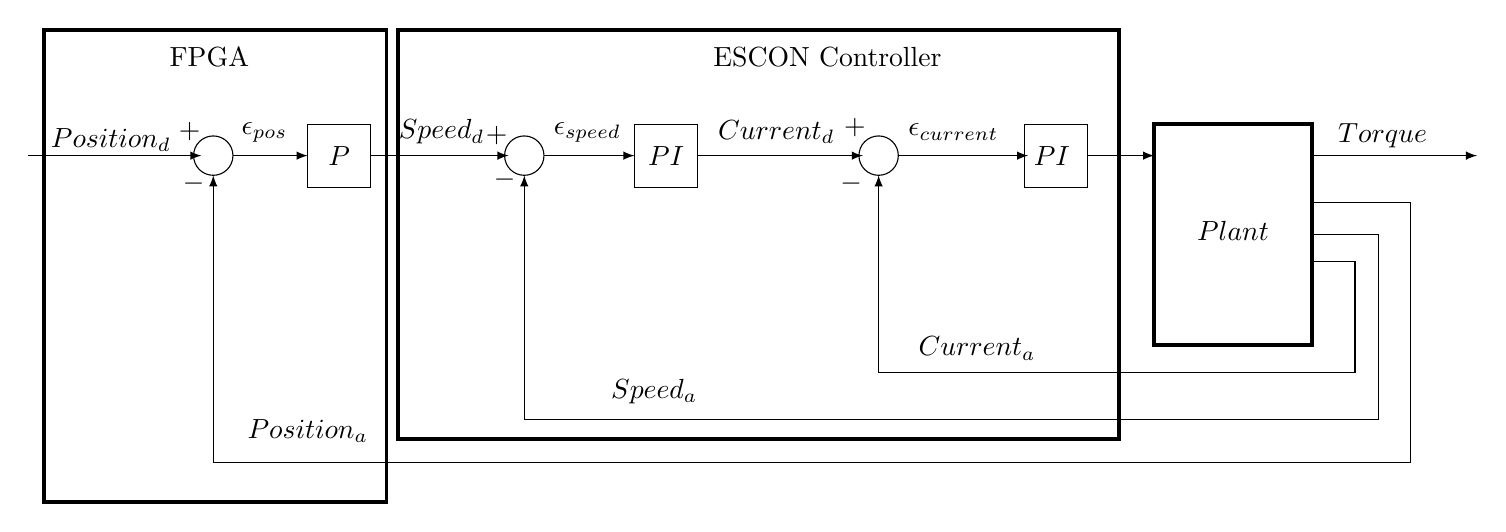
\begin{tikzpicture}%[transform canvas={scale=0.5}]

\draw [-latex] (10.6,3.4) ellipse (0.25 and 0.25);
\node at (7.9,3.4) {\normalsize{$PI$}};
\node at (12.8,3.4) {\normalsize{$PI$}};
\node at (17,3.65) {\normalsize{$Torque$}};
\node at (15.1,2.45) {\normalsize{$Plant$}};
\draw [-latex] (7.5,3.8) rectangle (8.3,3);
\draw [-latex] (12.45,3.8) rectangle (13.25,3);
\draw [-latex](8.3,3.4) -- (10.4,3.4);
\draw [-latex] (6.1,3.4) ellipse (0.25 and 0.25);
\draw [-latex](6.35,3.4) -- (7.5,3.4);
\node at (6.9,3.7) {$\epsilon_{speed}$};
\node at (11.55,3.7) {$\epsilon_{current}$};
\node at (3.75,3.4) {\normalsize{$P$}};
\draw [-latex] (3.35,3.8) rectangle (4.15,3);
\draw [-latex](4.15,3.4) -- (5.9,3.4);

\draw [-latex](10.85,3.4) -- (12.5,3.4);
\draw [-latex](13.25,3.4) -- (14.1,3.4);
\draw [-latex](16.1,3.4) -- (18.2,3.4);

\draw [-latex](16.1,2.05) -- (16.65,2.05) -- (16.65,0.65)-- (10.6,0.65)-- (10.6,3.15);
\draw [-latex](16.1,2.4) -- (16.95,2.4) -- (16.95,0.05)-- (6.1,0.05)-- (6.1,3.15);
\draw [-latex](16.1,2.8) -- (17.35,2.8) -- (17.35,-0.5)-- (2.15,-0.5)-- (2.15,3.15);

\node at (10.3,3.75) {$+$};
\node at (10.25,3.05) {$-$};

\draw [-latex] (2.15,3.4) ellipse (0.25 and 0.25);
\draw [-latex](2.4,3.4) -- (3.35,3.4);
\node at (5.85,3.1) {$-$};

\draw [-latex](-0.2,3.4) -- (2,3.4);
\node at (0.85,3.6) {$Position_d$};
\node at (2.1,4.65) {FPGA};
\node at (9.95,4.65) {ESCON Controller};
\node at (1.9,3.05) {$-$};
\node at (2.8,3.7) {$\epsilon_{pos}$};
\node at (5.05,3.7) {$Speed_d$};
\node at (9.3,3.7) {$Current_d$};
\node at (11.85,0.95) {$Current_a$};
\node at (7.75,0.4) {$Speed_a$};
\node at (3.35,-0.1) {$Position_a$};


\node (v2) at (1.85,3.7) {$+$};
\node (v2) at (5.75,3.65) {$+$};
\draw  [line width=0.5mm](14.1,3.8) rectangle (16.1,1);
\draw  [line width=0.5mm](0,5) rectangle (4.35,-1);
\draw [line width=0.5mm] (4.5,5) rectangle (13.65,-0.2);
\end{tikzpicture}
}
\caption{Embedded cascade control structure. d index means the desired control value, a index means actual value, $\epsilon$ is the error}
\label{cascade_fig}
\end{figure}


\subsubsection{FPGA}

The FPGA built into the sbRIO is taking care of the interfacing between the controllers and the microprocessor. The code running on the FPGA is much faster than the one running on the microprocessor. To reach maximum possible speed, we implemented whatever we could on the FPGA, however the FPGA is incapable of handling higher level functions such as string handling and UDP networking.

The FPGA's main functions are the following:

\begin{itemize}	
	\setlength\itemsep{0em}
	\item Count the encoder ticks coming from the controller
	\item Read the controller's analog and digital inputs 
	\item Calculate position PID control signal and send the corresponding PWM signal to the controller
	\item Enable the motors
	
\end{itemize}

Since the current value coming from the ESCON is noisy, the FPGA also needs a built in low pass filter.

\subsubsection{ESCON motor controllers}
\label{escon_con}

The ESCON controllers are programmed to output a speed corresponding to the FPGA PWM signal. The speed controller has an inner current controller, which also keeps the motors from taking overcurrent. The current ramps can be adjusted to fit the user's needs. The speed control gain can be adjusted by the onboard potmeter. 
The outer speed loop provides the control signal for the internal current controller. The inner control loop must have a higher frequency than the speed control loop. The PI current controller is running at 53.6 kHz, while the PI speed controller is running at 5.36 kHz. The inner loop ensures fast response, the outer higher precision ($http://www.iraj.in/journal/journal_file/journal_pdf/1-59-140229369778-81.pdf$). The advantages of the cascade structure:

\begin{itemize}
	\item Better setpoint tracking
	\item Better disturbance rejection
	\item Less delay and phase lag
\end{itemize}

The position is controlled by setting the duty ratio of the incoming PWM signal. The speed reference is 0 at 50\% duty ratio and grows linearily at higher values.
The ESCON controller has 2 programmable analog outputs, thus we are unable to read speed, actual current and demand current simultaneously.
The controllers have autocalibration functionalities, but this ability is obstructed by the gearing limits.

ESCON Studio provides the tool for logging data from the ESCON controller by using only a USB cable.
\section{Mapping}

The setup studied in this project does not allow the translations of the EndoWrist. Although the models derived can be used on the full da Vinci robot, the mapping of the movements of the Geomagic Touch to the tool cannot be the same. As described in \secref{sec:geo_magic}, the GT can only actuates three joints, these joints are the one that needs to be used for the human to easily estimates the quality of the force feedback. It was decided to control the EndoWrist by controlling the roll, pitch and clamping independently. To do so, each of these three joints are assigned one vector. All three vectors are orthogonal to be able to sense the feedback of each joint individually.
The roll of the EndoWrist was associated to the roll of the GT. The clamp of the EndoWrist is associated to the radial vector going from the base of the GT to the end of the stylus. The pitch is controlled by the normal vector to the plan defined by the two previous vectors which is a vertical vector. The vectors in the horizontal plan are represented in \figref{fig:cartesian_polar}. The Cartesian z axis and the vector for the pitch of the EndoWrist are collinear and are not represented on the figure.
\\

\begin{figure}[H]
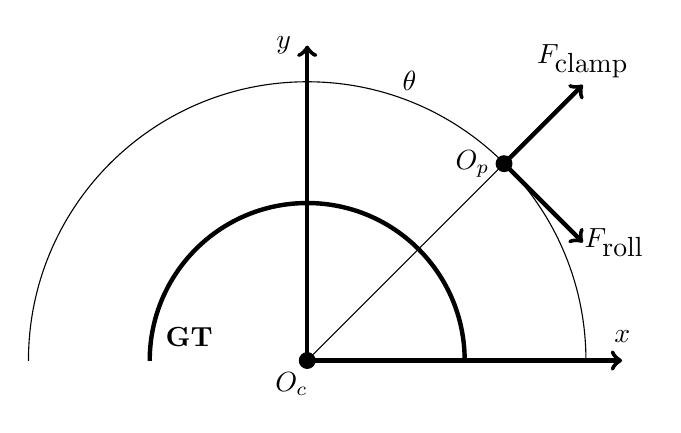
\begin{tikzpicture}
	% GT
	\begin{scope}
	    \clip (-2.1,0) rectangle (2.1,2.1);
	    \draw (0,0) circle(2)[ultra thick];
	\end{scope}
	\node at (-1.5,0.3) {$\textbf{GT}$};
	%Cartesian axis
	\draw [fill=black] (-0,-0) circle [radius=0.1];
	\draw [->,ultra thick] (0,0) -- (0,4);
	\draw [->,ultra thick] (0,0) -- (4,0);
	\node at (-0.3, 4) {$y$};
	\node at (4, 0.3) {$x$};
	\node at (-0.2, -0.3) {$O_c$};
	%end effector
	\draw [fill=black] (2.5,2.5) circle [radius=0.1];
	\begin{scope}
	    \clip (-3.55,0) rectangle (3.55,3.55);
	    \draw (0,0) circle(3.54);
	\end{scope}
	\draw (0,0) -- (2.5,2.5);
	\node at (2.1, 2.5) {$O_p$};
	%Cylindrical axis
	\draw [->,ultra thick] (2.5,2.5) -- (3.5,3.5);
	\draw [->,ultra thick] (2.5,2.5) -- (3.5,1.5);
	\node at (3.5,3.8) {$F_\textrm{clamp}$};
	\node at (3.9,1.5) {$F_\textrm{roll}$};
	\node at (1.3,3.55) {$\theta$};

\end{tikzpicture}
\label{fig:cartesian_polar}
\caption{Vectors in the Cartesian plan}
\end{figure}
with:\\
	\hspace*{8mm} $O_c$ Origin of the Cartesian space
	\space*{8mm} $O_p$ Position of the end-effector


The phantom\_omni node\cite{phantom_omni_github} used to communicate can only handle Cartesian positions and forces. Thus, conversion from cylindrical to Cartesian and from Cartesian to cylindrical are required, this transformation are described in \eqref{eq:cartesian_to_cylindrical} and \eqref{eq:cylindrical_to_cartesian}.



\begin{equation} 
\begin{split}
	F_x &= F_\textrm{clamp}\cdot sin(\theta) + F_\textrm{roll}\cdot cos(\theta)\\
	F_y &= F_\textrm{clamp}\cdot cos(\theta) - F_\textrm{roll}\cdot sin(\theta)\\
	F_z &= F_\textrm{pitch}
	\end{split}
\label{eq:cylindrical_to_cartesian}
\end{equation}
with:\\
\hspace*{8mm} $\theta = atan2(y,x)$\\
\hspace*{8mm} (x,y,z)  the Cartesian coordinates of the GT\\
\hspace*{8mm} $F_\textrm{clamp}$  the force feedback from the clamp\\
\hspace*{8mm} $F_\textrm{pitch}$  the force feedback from the pitch\\
\hspace*{8mm} $F_\textrm{roll}$  the force feedback from the roll\\

\begin{equation} 
1+1=\pi;
\label{eq:cartesian_to_cylindrical}
\end{equation}


